% Options for packages loaded elsewhere
\PassOptionsToPackage{unicode}{hyperref}
\PassOptionsToPackage{hyphens}{url}
\PassOptionsToPackage{dvipsnames,svgnames,x11names}{xcolor}
%
\documentclass[
  11pt,
  krantz2, a4paper, twoside]{krantz}
\usepackage{amsmath,amssymb}
\usepackage{lmodern}
\usepackage{setspace}
\usepackage{iftex}
\ifPDFTeX
  \usepackage[T1]{fontenc}
  \usepackage[utf8]{inputenc}
  \usepackage{textcomp} % provide euro and other symbols
\else % if luatex or xetex
  \usepackage{unicode-math}
  \defaultfontfeatures{Scale=MatchLowercase}
  \defaultfontfeatures[\rmfamily]{Ligatures=TeX,Scale=1}
\fi
% Use upquote if available, for straight quotes in verbatim environments
\IfFileExists{upquote.sty}{\usepackage{upquote}}{}
\IfFileExists{microtype.sty}{% use microtype if available
  \usepackage[]{microtype}
  \UseMicrotypeSet[protrusion]{basicmath} % disable protrusion for tt fonts
}{}
\makeatletter
\@ifundefined{KOMAClassName}{% if non-KOMA class
  \IfFileExists{parskip.sty}{%
    \usepackage{parskip}
  }{% else
    \setlength{\parindent}{0pt}
    \setlength{\parskip}{6pt plus 2pt minus 1pt}}
}{% if KOMA class
  \KOMAoptions{parskip=half}}
\makeatother
\usepackage{xcolor}
\usepackage{longtable,booktabs,array}
\usepackage{calc} % for calculating minipage widths
% Correct order of tables after \paragraph or \subparagraph
\usepackage{etoolbox}
\makeatletter
\patchcmd\longtable{\par}{\if@noskipsec\mbox{}\fi\par}{}{}
\makeatother
% Allow footnotes in longtable head/foot
\IfFileExists{footnotehyper.sty}{\usepackage{footnotehyper}}{\usepackage{footnote}}
\makesavenoteenv{longtable}
\usepackage{graphicx}
\makeatletter
\def\maxwidth{\ifdim\Gin@nat@width>\linewidth\linewidth\else\Gin@nat@width\fi}
\def\maxheight{\ifdim\Gin@nat@height>\textheight\textheight\else\Gin@nat@height\fi}
\makeatother
% Scale images if necessary, so that they will not overflow the page
% margins by default, and it is still possible to overwrite the defaults
% using explicit options in \includegraphics[width, height, ...]{}
\setkeys{Gin}{width=\maxwidth,height=\maxheight,keepaspectratio}
% Set default figure placement to htbp
\makeatletter
\def\fps@figure{htbp}
\makeatother
\setlength{\emergencystretch}{3em} % prevent overfull lines
\providecommand{\tightlist}{%
  \setlength{\itemsep}{0pt}\setlength{\parskip}{0pt}}
\setcounter{secnumdepth}{5}
\newlength{\cslhangindent}
\setlength{\cslhangindent}{1.5em}
\newlength{\csllabelwidth}
\setlength{\csllabelwidth}{3em}
\newlength{\cslentryspacingunit} % times entry-spacing
\setlength{\cslentryspacingunit}{\parskip}
\newenvironment{CSLReferences}[2] % #1 hanging-ident, #2 entry spacing
 {% don't indent paragraphs
  \setlength{\parindent}{0pt}
  % turn on hanging indent if param 1 is 1
  \ifodd #1
  \let\oldpar\par
  \def\par{\hangindent=\cslhangindent\oldpar}
  \fi
  % set entry spacing
  \setlength{\parskip}{#2\cslentryspacingunit}
 }%
 {}
\usepackage{calc}
\newcommand{\CSLBlock}[1]{#1\hfill\break}
\newcommand{\CSLLeftMargin}[1]{\parbox[t]{\csllabelwidth}{#1}}
\newcommand{\CSLRightInline}[1]{\parbox[t]{\linewidth - \csllabelwidth}{#1}\break}
\newcommand{\CSLIndent}[1]{\hspace{\cslhangindent}#1}
%\usepackage{tikz-cd} % \xleftrightarrow
%\usepackage{amsmath} 
%\documentclass[b5paper,9pt]{extarticle}
%\usepackage{geometry}

%\usepackage[%
%  b5, % <===============================================================
%  center, cam
%  %axes,cross,pdftex,center
%]{crop}

\usepackage{graphicx}
%\usepackage{polyglossia}
%\usepackage{ctex}
%\usepackage{fontspec}
%\usepackage{xetexko}
%\setmainfont{NanumMyeongjo}
\setmainfont{Noto Serif CJK KR}
%\setmainhangulfont{Noto Serif CJK KR} 
%\setmainhangulfont{NanumMyeongjo}
%\setmainhanjafont{Noto Serif CJK KR}[Language=Chinese Simplified]
%\setmainhanjafont{Noto Serif CJK KR}
\usepackage{kotex}
\setmonohangulfont{NanumGothicCoding}

%sungpil defined above

\usepackage{booktabs}
\usepackage{longtable}
\usepackage[bf,singlelinecheck=off]{caption}

%\usepackage[utf8]{inputenc}

%\usepackage{xeCJK}
%\setCJKmainfont[$for(CJKoptions)$$CJKoptions$$sep$,$endfor$]{$CJKmainfont$}

%\usepackage{xeCJK}
%\setCJKmainfont{SimSun}

%\usepackage{xeCJK}
%\setCJKmainfont{SimSun}
%\setmainfont{Calibri}
%\setCJKmainfont{宋体}

%\setmainhanjafont{SimSun}
%\setmainfont[UprightFeatures={SmallCapsFont=AlegreyaSC-Regular}]{Alegreya}

%\setmainhanjafont[
%  BoldFont=*, BoldFeatures={FakeBold=2},
%  ItalicFont=*, ItalicFeatures={FakeSlant=0.17},
%  SlantedFont=*, SlantedFeatures={FakeSlant=0.17},
%  BoldItalicFont=*, BoldItalicFeatures={FakeBold=2,FakeSlant=0.17},
%  BoldSlantedFont=*, BoldSlantedFeatures={FakeBold=2,FakeSlant=0.17},
%]{SimSun}

\usepackage{framed,color}
\definecolor{shadecolor}{RGB}{248,248,248}

\renewcommand{\textfraction}{0.05}
\renewcommand{\topfraction}{0.8}
\renewcommand{\bottomfraction}{0.8}
\renewcommand{\floatpagefraction}{0.75}

\renewenvironment{quote}{\begin{VF}}{\end{VF}}
\let\oldhref\href
\renewcommand{\href}[2]{#2\footnote{\url{#1}}}

\ifxetex
  \usepackage{letltxmacro}
  \setlength{\XeTeXLinkMargin}{1pt}
  \LetLtxMacro\SavedIncludeGraphics\includegraphics
  \def\includegraphics#1#{% #1 catches optional stuff (star/opt. arg.)
    \IncludeGraphicsAux{#1}%
  }%
  \newcommand*{\IncludeGraphicsAux}[2]{%
    \XeTeXLinkBox{%
      \SavedIncludeGraphics#1{#2}%
    }%
  }%
\fi

\makeatletter
\newenvironment{kframe}{%
\medskip{}
\setlength{\fboxsep}{.8em}
 \def\at@end@of@kframe{}%
 \ifinner\ifhmode%
  \def\at@end@of@kframe{\end{minipage}}%
  \begin{minipage}{\columnwidth}%
 \fi\fi%
 \def\FrameCommand##1{\hskip\@totalleftmargin \hskip-\fboxsep
 \colorbox{shadecolor}{##1}\hskip-\fboxsep
     % There is no \\@totalrightmargin, so:
     \hskip-\linewidth \hskip-\@totalleftmargin \hskip\columnwidth}%
 \MakeFramed {\advance\hsize-\width
   \@totalleftmargin\z@ \linewidth\hsize
   \@setminipage}}%
 {\par\unskip\endMakeFramed%
 \at@end@of@kframe}
\makeatother

\makeatletter
\@ifundefined{Shaded}{
}{\renewenvironment{Shaded}{\begin{kframe}}{\end{kframe}}}
\makeatother

\newenvironment{rmdblock}[1]
  {
  \begin{itemize}
  \renewcommand{\labelitemi}{
    \raisebox{-.7\height}[0pt][0pt]{
      {\setkeys{Gin}{width=3em,keepaspectratio}\includegraphics{images/#1}}
    }
  }
  \setlength{\fboxsep}{1em}
  \begin{kframe}
  \item
  }
  {
  \end{kframe}
  \end{itemize}
  }
\newenvironment{rmdnote}
  {\begin{rmdblock}{note}}
  {\end{rmdblock}}
\newenvironment{rmdcaution}
  {\begin{rmdblock}{caution}}
  {\end{rmdblock}}
\newenvironment{rmdimportant}
  {\begin{rmdblock}{important}}
  {\end{rmdblock}}
\newenvironment{rmdtip}
  {\begin{rmdblock}{tip}}
  {\end{rmdblock}}
\newenvironment{rmdwarning}
  {\begin{rmdblock}{warning}}
  {\end{rmdblock}}

\usepackage{makeidx}
\makeindex

\urlstyle{tt}

%https://tex.stackexchange.com/questions/85400/how-to-change-space-around-theorem-environments

\usepackage{amsthm}
\makeatletter
\def\example@space@setup{%
  \example@preskip=0.001cm
  \example@postskip=\thm@preskip
}
\makeatother

%https://github.com/rstudio/bookdown/issues/901
\usepackage{caption}
\captionsetup[figure]{labelsep=period}
\captionsetup[table]{labelsep=period}

\frontmatter
\usepackage{kotex}
\usepackage{chemarr}
\usepackage{booktabs}
\usepackage{longtable}
\usepackage{array}
\usepackage{multirow}
\usepackage{wrapfig}
\usepackage{float}
\usepackage{colortbl}
\usepackage{pdflscape}
\usepackage{tabu}
\usepackage{threeparttable}
\usepackage{threeparttablex}
\usepackage[normalem]{ulem}
\usepackage{makecell}
\usepackage{xcolor}
\ifLuaTeX
  \usepackage{selnolig}  % disable illegal ligatures
\fi
\IfFileExists{bookmark.sty}{\usepackage{bookmark}}{\usepackage{hyperref}}
\IfFileExists{xurl.sty}{\usepackage{xurl}}{} % add URL line breaks if available
\urlstyle{same} % disable monospaced font for URLs
\hypersetup{
  pdfauthor={가톨릭대학교 계량약리학연구소(PIPET), AIMS BioScience, Q-fitter - Ver 0.0.1 (2022-06-03)},
  colorlinks=true,
  linkcolor={Maroon},
  filecolor={Maroon},
  citecolor={Blue},
  urlcolor={Blue},
  pdfcreator={LaTeX via pandoc}}

\title{신약개발을 위한 실전 약동학 II

(ADME의 기초 자료)}
\author{가톨릭대학교 계량약리학연구소(PIPET), AIMS BioScience, Q-fitter - Ver 0.0.1 (2022-06-03)}
\date{2022-09-14}

\begin{document}
\maketitle

%sungpil added above

%\cleardoublepage\newpage\thispagestyle{empty}\null
%\cleardoublepage\newpage\thispagestyle{empty}\null
%\cleardoublepage\newpage

\newpage

\thispagestyle{empty}

\begin{center}
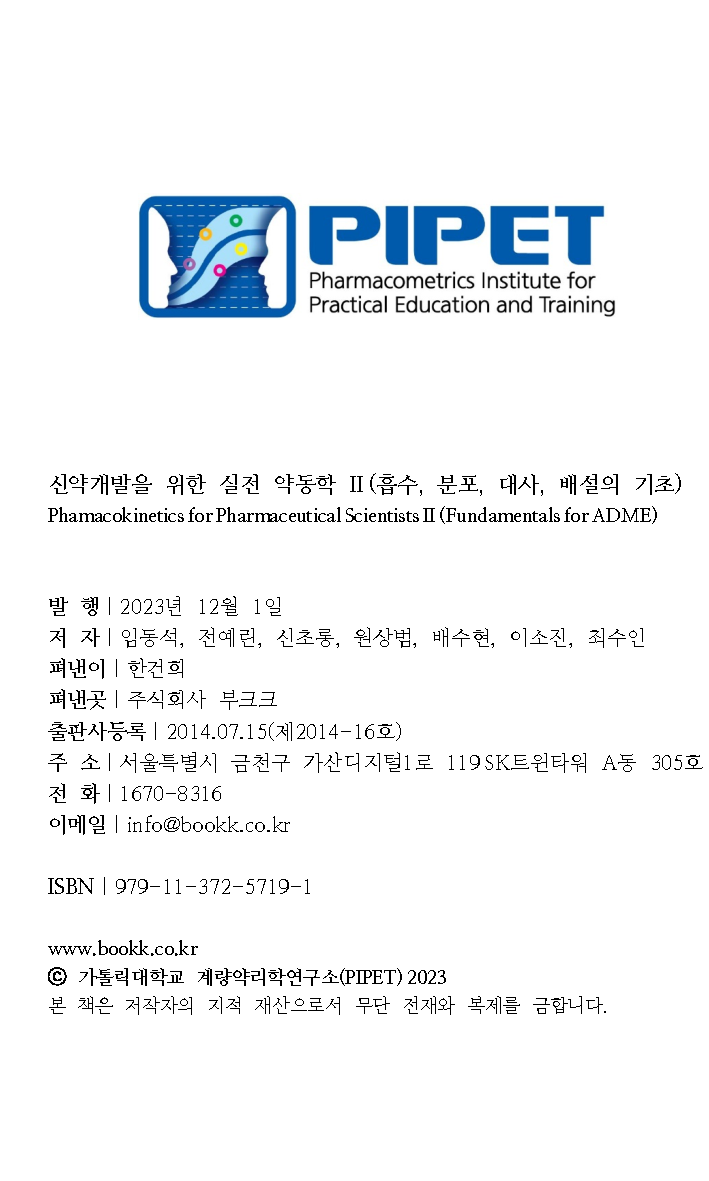
\includegraphics{images/pipet.pdf}
\end{center}

\thispagestyle{empty}
%\scriptsize
%\hfill Ver. 20200801
%\normalsize
\begin{center}
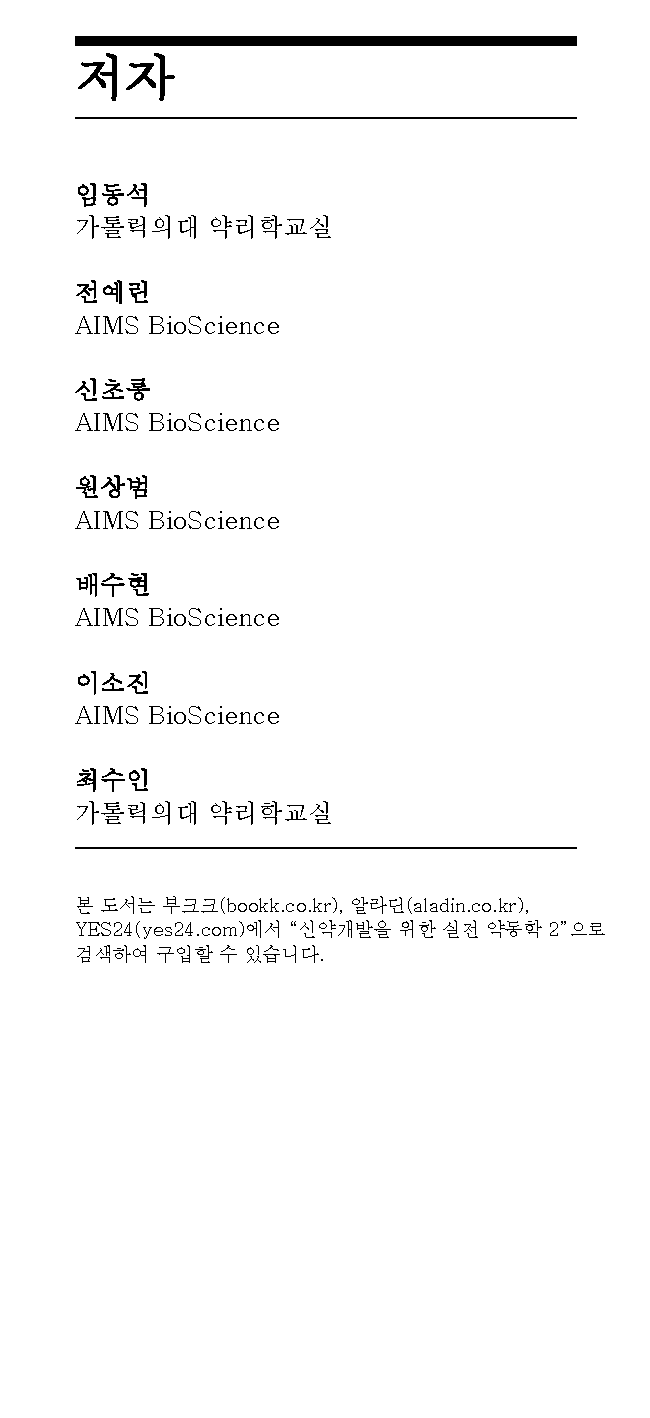
\includegraphics{images/authors.pdf}
\end{center}

\setlength{\abovedisplayskip}{-5pt}
\setlength{\abovedisplayshortskip}{-5pt}

\newpage\thispagestyle{empty}\null

{
\hypersetup{linkcolor=}
\setcounter{tocdepth}{2}
\tableofcontents
}
\setstretch{1.3}
\hypertarget{uxba38uxb9acuxb9d0}{%
\chapter*{머리말}\label{uxba38uxb9acuxb9d0}}


\normalsize

이 책은 제약·바이오 업계의 신약 연구자들이 약동학(pharmacokinetics)을 이해하는 것을 돕기 위해 만들어졌습니다.\index{약동학}

\index{약동학}\index{약동학}\index{약력학} \index{임상개발} \index{의사결정}
약동학은 신약의 발견부터 시판허가 이후의 관리에 이르기까지 모든 단계에서 쓰이는 가장 기본적이고 필수적인 지식이며 도구입니다.
오늘날 다양한 생명과학 분야의 전문인력들이 우리나라에서 신약의 발견과 초기개발과정, 임상개발 과정에서 핵심적인 역할들을 수행하고 있습니다.
그러나 학위과정 중에 약동학이나 약력학을 공부할 기회가 없었던 분들이 많아서 업무 수행 중 의사결정이나 소통에 있어서 늘 크고 작은 어려움을 겪고 있습니다.
이런 현실은 본격적인 신약개발의 역사가 일천한 우리나라에서 거쳐갈 수밖에 없는 과정이지만, 소수의 전문가들이 제약회사에 가서 강의 몇시간 하는 식으로는 해결되지 않습니다.

물론 `임상약동학' 또는 `약동학' 이라는 제목의 좋은 책들은 이미 국내에도\index{약동학}
여러 권 나와 있습니다. 그러나 약동학 데이터를 직접 들여다보고 분석하는\index{약동학}
학문(임상약리학, 약제학 등)을 대학원에서 전공하지 않은 이상, 그 두꺼운 교재들의 복잡한 수식을 다 읽어야 할 절박함도 없을 것이고, 설혹 읽어본다
한들 쉽게 이해할 수도 없습니다.
또한 많은 책들이 약동학 수식들을 충실히\index{약동학}
다루고는 있지만 신약을 실제로 개발하는 과정에서 제약사 연구원들이 부딪히는 의문들을 해결하는데 주안점을 두고 저술된 것이 아니므로 현장의 답답함을 풀어주는 데에는 한계가 있어왔습니다.

이런 현실을 조금이라도 타개하기 위해서는 국내 제약, 바이오 기업에서 신약개발 업무를 수행하고 있는 다양한 전공의 연구자들이 시공간의 제약없이 공부할 수 있는 온라인 강의 동영상, 그리고 그와 함께 읽을 수 있는 교재를 만드는 작업이 절실하였습니다.
그래서 저자들은 지난 20여년간 대학과 기업의 연구원들을 대상으로 약동학을 가르치며 겪은 학습자들의 질문과 반응들을 토대로 꼭 필요한 내용들을 이해하기 쉽게 설명하고자 영상 제작과 함께, 이 교재를 만들게 되었습니다. \footnote{\url{http://pipetlms.or.kr}}

저자들은 ``약동학''이라는 방법론 자체를 전공했다기 보다는 그것을 기본적인\index{약동학}
도구로 사용하는 학문인 임상약리학을 공부해 온 사람들입니다. 이 책에 담긴
지식들 중 저자들이 새롭게 만들어낸 것은 거의 없으므로 이 책은 오랜 세월
동안 세상의 많은 학자들이 만들어 온 지식들을 모아서 시중에 유통시킨 것에
지나지 않습니다. 다만 신약개발을 위해 임상약리학을 적용하는 과정에서,
함께 일해왔던 기업들에서 만들어진 물질들의 약효, 독성, 약동학에 관한\index{약동학}
비임상, 임상 연구자료들을 들여다보면서 수없이 토의하고 질문했던 내용들을
책 속에 충실히 반영하고자 하였습니다. 그 내용을 독자들이 좀 더
효율적으로 학습할 수 있도록 오래된 지식들을 새로운 방식으로 자르고 묶고
다듬어 내놓고자 노력했습니다. 약동학 책에는 수식들이 꽤 등장하기 때문에, 이 책의 내용 역시 어렵게 느껴질 수 있으므로 온라인상에 공개되어 있는 강의 동영상을 책과 함께 공부하시기를 권합니다.
이 책은 제약/바이오 기업의 연구자를 대상으로 쓰여진 것이지만, 관련된 전공을 공부하는 대학원생들에게도 도움이 될 것입니다.
그러므로 학생들의 책값 부담을 덜어주기 위해 책 전체를 웹북과 pdf로 온라인 상에 공개하였습니다. \footnote{\url{http://pipet.or.kr/books/pharmapk}}
종이책은 print on demand 방식으로 출판하면서 저자들은 인세를 받지 않음으로써 복사/제본비 수준의 책값을 책정하였습니다.

이를 위해 원고 집필 뿐 아니라 책의 조판에까지 많은 시간과 수고를 쏟아야 했던 한성필 교수님께 고마움을 전합니다.

이 책과 강의동영상이 우리나라에서 신약의 비임상, 임상개발 과정에 참여하고 있는 각 분야 전문가들의 역량을 더욱 잘 발휘할 수 있게 돕는 디딤돌이 된다면 저자들 모두의 기쁨이겠습니다.
\index{임상개발}

\hfill 2022년 9월, 성의교정 연구실에서

\hfill 대표저자 임동석 拜

\normalsize

\mainmatter

\hypertarget{part-uxbb3cuxb9acuxd654uxd559uxc801-uxc131uxc9c8}{%
\part{물리화학적 성질}\label{part-uxbb3cuxb9acuxd654uxd559uxc801-uxc131uxc9c8}}

\hypertarget{uxc6a9uxd574uxb3c4}{%
\chapter{용해도}\label{uxc6a9uxd574uxb3c4}}

\Large\hfill

전예린
\normalsize

\hypertarget{uxc11cuxb860}{%
\section{서론}\label{uxc11cuxb860}}

용해도(solubility)는 약물의 흡수에 관여하는 요소로 생체이용률에 영향을 줄 수 있어 신약개발 과정에서 매우 중요하다. 우리가 정제 혹은 캡슐 등의 형태인 약을 경구로 투여했을 때 유효 성분의 약물은 붕해(disintegration), 용해(dissolution) 및 확산(diffusion) 과정을 거쳐 전신 순환혈에 흡수된다 (그림 \ref{fig:01-01}).

\begin{figure}

{\centering 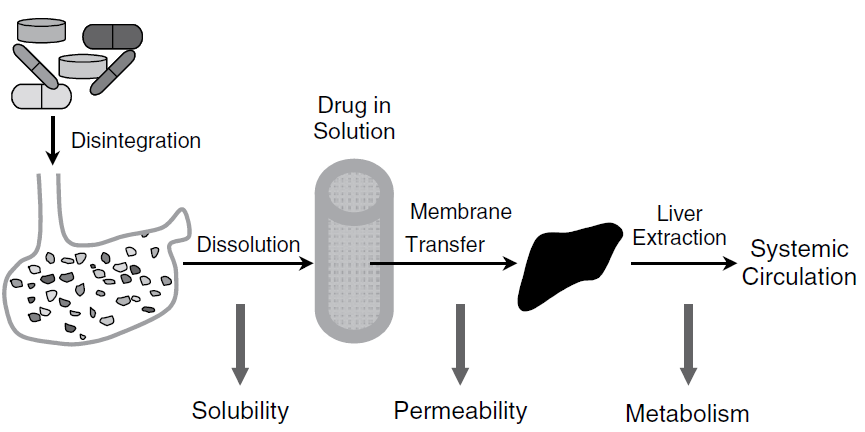
\includegraphics[width=1\linewidth]{media-01/image1} 

}

\caption{약물의 흡수 과정 (\protect\hyperlink{ref-di2015drug}{Di and Kerns 2015})}\label{fig:01-01}
\end{figure}



약물이 흡수되기 위해서는 반드시 용해되어야 하고, 여기서 약물이 용해되는 정도가 바로 용해도이다. 용해도가 높은 약물은 위장관에서의 약물 농도가 높아지고, 더 많은 양의 약물이 장 상피세포의 표면적과 만나게 되므로 더욱 많이 흡수된다. 즉, 용해도가 높을수록 단위시간 당 단위면적에서 흡수되는 약물의 양이 많아진다 (Fick's law 제 1법칙). 반면, 용해도가 낮은 난용성 약물은 용해 및 흡수가 잘 되지 않아 낮은 생체이용률을 보이게 된다. 따라서 ``용해도''는 약물의 흡수에 영향을 주는 매우 중요한 인자라고 할 수 있다.

신약개발 과정 중 약물의 약리, 독성 및 PK에 관련된 다양한 평가를 진행할 때 약물의 용해도는\emph{in vitro} assay 평가 농도 혹은 \emph{in vivo} 시험의 부형제 선정에 중요한 단서를 제공할 수 있다. 예를 들면, 난용성 약물의 경우 \emph{in vitro} assay의 buffer나 media에 약물을 고농도로 처리 시 침전 현상으로 인해 농도 의존적인 결과를 확인할 수 없는 경우가 있다. 뿐만 아니라 \emph{in vivo} 시험에서도 약효나 독성에 영향을 미치지 않은 부형제를 사용해야 하는 약효 및 독성 시험 또는 clear solution형태로 주사하여야 하는 정맥투여 PK 시험을 수행할 때 낮은 용해도로 인해 어려움을 겪는 경우도 많다.

이렇듯 용해도는 신약개발 과정에서 필수적으로 확인해야 할 약물의 특성이므로, 이 장에서는 용해도에 대한 개념, 기준 및 영향을 줄 수 있는 인자 등에 대해 자세히 기술하여 이해를 돕고자 한다.

\hypertarget{uxc6a9uxd574uxb3c4-uxbd84uxb958-uxae30uxc900}{%
\section{용해도 분류 기준}\label{uxc6a9uxd574uxb3c4-uxbd84uxb958-uxae30uxc900}}

``개발하고자 하는 약물의 목표 용해도가 있는가?'' 혹은 ``약물의 용해도의 좋고 나쁨의 기준이 있는가?''에 대한 문의가 있다면 안타깝게도 이에 대한 대답은 ``명확한 기준은 없다''이다. 그 이유는 약물의 투과도 (Permeability), 평가하고자 하는 약물의 농도 혹은 용량, 시험 항목 혹은 목적 등과 같은 다양한 요인에 따라 목표로 하는 용해도와 그 기준이 결정될 것이기 때문이다. 따라서 이 절에서는 신약개발 단계 별로 용해도의 분류 기준을 나눠보고자 한다.

Drug discovery 단계에서 화합물을 합성하는 연구자들은 통상적으로 다음과 같은 기준으로 용해도를 분류한다 (표 \ref{tab:table01-01}).

\begin{longtable}[]{@{}
  >{\raggedright\arraybackslash}p{(\columnwidth - 2\tabcolsep) * \real{0.3056}}
  >{\raggedright\arraybackslash}p{(\columnwidth - 2\tabcolsep) * \real{0.3056}}@{}}
\caption{\label{tab:table01-01} Drug discovery 단계에서의 용해도 분류 기준}\tabularnewline
\toprule()
\begin{minipage}[b]{\linewidth}\raggedright
Solubility (μg/mL)
\end{minipage} & \begin{minipage}[b]{\linewidth}\raggedright
Criteria
\end{minipage} \\
\midrule()
\endfirsthead
\toprule()
\begin{minipage}[b]{\linewidth}\raggedright
Solubility (μg/mL)
\end{minipage} & \begin{minipage}[b]{\linewidth}\raggedright
Criteria
\end{minipage} \\
\midrule()
\endhead
\textless10 & Low \\
10-60 & Moderate \\
\textgreater60 & High \\
\bottomrule()
\end{longtable}

Drug development 단계에서는 대한약전 및 USP에 용해도의 분류 기준이 다음과 같이 정의되어 있다. ``고체의 경우, 가루로 한 다음 용매 중에 넣고 20±5℃에서 5분마다 30초간씩 세게 흔들어 섞을 때 30분 이내에 녹는 정도''가 용해도이며, 용질 1 g 또는 1 mL를 녹이는데 필요한 용매의 양에 따라 다음과 같이 용해도를 분류할 수 있다 (표 \ref{tab:table01-02}).

\begin{longtable}[]{@{}
  >{\raggedright\arraybackslash}p{(\columnwidth - 4\tabcolsep) * \real{0.3056}}
  >{\raggedright\arraybackslash}p{(\columnwidth - 4\tabcolsep) * \real{0.3056}}
  >{\raggedright\arraybackslash}p{(\columnwidth - 4\tabcolsep) * \real{0.3750}}@{}}
\caption{\label{tab:table01-02} 대한약전 및 USP에서의 용해도 분류 기준}\tabularnewline
\toprule()
\begin{minipage}[b]{\linewidth}\raggedright
대한약전 용어
\end{minipage} & \begin{minipage}[b]{\linewidth}\raggedright
USP 용어
\end{minipage} & \begin{minipage}[b]{\linewidth}\raggedright
용질 1g 또는 1 mL를
녹이는데
필요한 용매의 양
\end{minipage} \\
\midrule()
\endfirsthead
\toprule()
\begin{minipage}[b]{\linewidth}\raggedright
대한약전 용어
\end{minipage} & \begin{minipage}[b]{\linewidth}\raggedright
USP 용어
\end{minipage} & \begin{minipage}[b]{\linewidth}\raggedright
용질 1g 또는 1 mL를
녹이는데
필요한 용매의 양
\end{minipage} \\
\midrule()
\endhead
썩 잘 녹는다 & Very soluble & 1 mL 미만 \\
잘 녹는다 & Freely soluble & 1 mL 이상 10 mL 미만 \\
녹는다 & Soluble & 10 mL 이상 30 mL 미만 \\
조금 녹는다 & Sparingly soluble & 30 mL 이상 100 mL 미만 \\
녹기 어렵다 & Slightly soluble & 100 mL 이상 1000 mL 미만 \\
매우 녹기 어렵다 & Very slightly
soluble & 1000 mL 이상 10000 mL
미만 \\
거의 녹지 않는다 & Practically soluble & 10000 mL 이상 \\
\bottomrule()
\end{longtable}

마지막으로 신약개발 과정에서 전반적으로 활용되는 용해도의 기준은 Biopharmaceutics Classification System (BCS)에 따른 분류이다 (그림 \ref{fig:01-02}). 이는 용해도 및 투과도에 따라 다음과 같이 4개의 class로서 약물의 특성을 분류한다.

\begin{itemize}
\tightlist
\item
  Class I: 높은 용해도, 높은 투과도
\item
  Class II: 낮은 용해도, 높은 투과도
\item
  Class III: 높은 용해도, 낮은 투과도
\item
  Class IV: 낮은 용해도, 낮은 투과도
\end{itemize}

Class I과 Class III로 분류되기 위한 ``높은 용해도''란 ``37℃ 및 pH 1.2-6.8 범위에서 1회 최대 복용량 (치료용량)을 30분 이내 용해시키기에 충분한 수용액의 부피가 250 mL 이하''일 때를 의미한다.
이 때 250 mL은 위장액의 부피 혹은 약물 복용 시 먹는 물 한 컵의 양을 기준으로 설정된 것이다.

\begin{figure}

{\centering 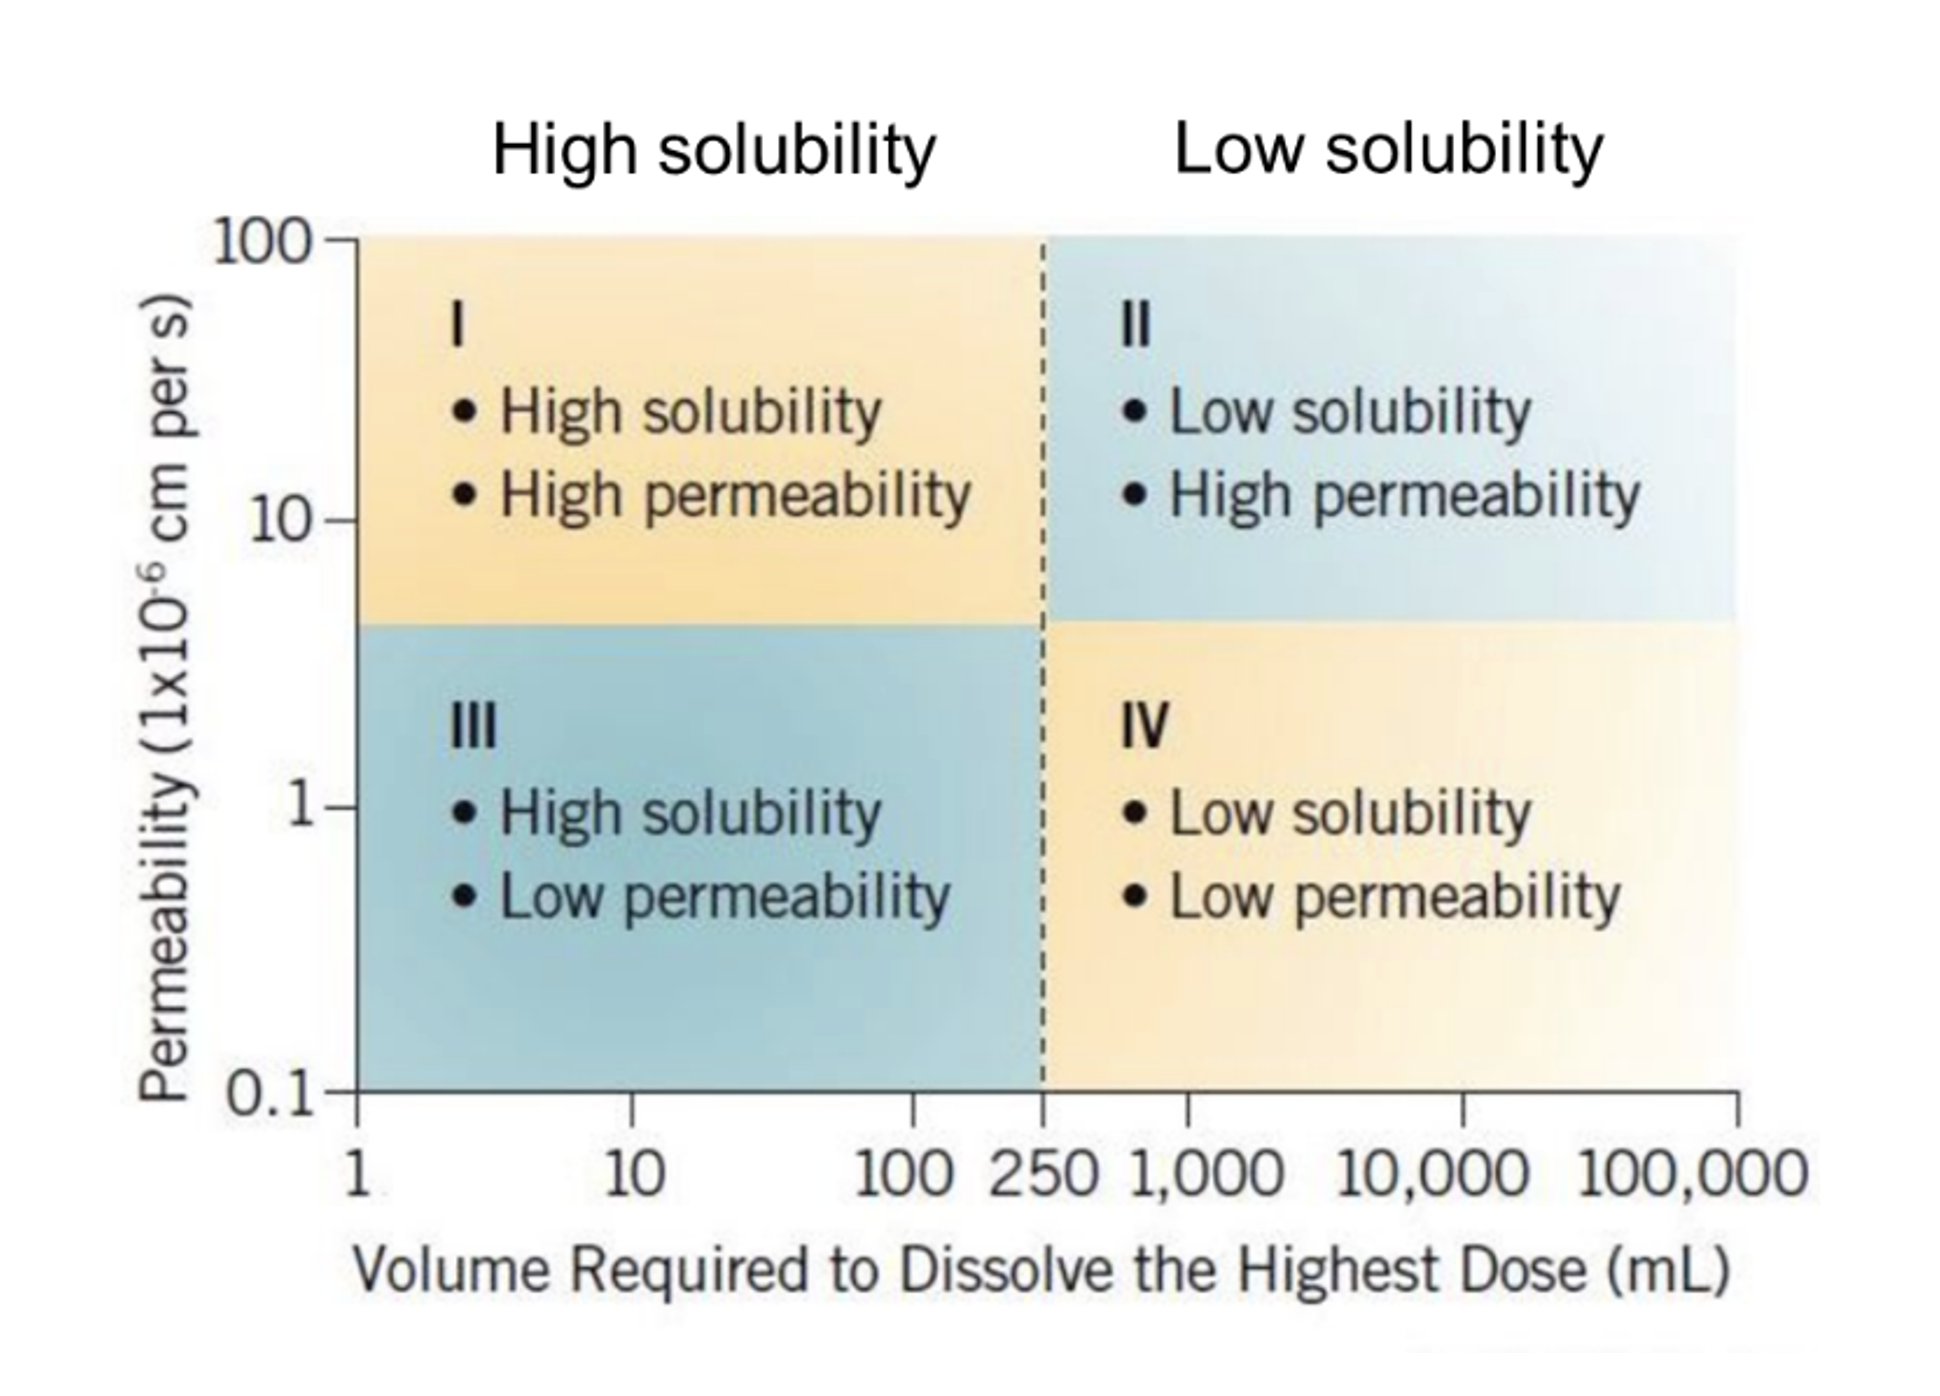
\includegraphics[width=1\linewidth]{media-01/image2} 

}

\caption{Biopharmaceutics Classification System (BCS)}\label{fig:01-02}
\end{figure}



\hypertarget{uxc6a9uxd574uxb3c4uxc5d0-uxc601uxd5a5uxc744-uxc8fcuxb294-uxc778uxc790}{%
\section{용해도에 영향을 주는 인자}\label{uxc6a9uxd574uxb3c4uxc5d0-uxc601uxd5a5uxc744-uxc8fcuxb294-uxc778uxc790}}

\hypertarget{uxc57duxbb3cuxc758-uxbb3cuxb9acuxd654uxd559uxc801-uxd2b9uxc131}{%
\subsection{약물의 물리화학적 특성}\label{uxc57duxbb3cuxc758-uxbb3cuxb9acuxd654uxd559uxc801-uxd2b9uxc131}}

용해도는 약물의 물리화학적 특성에 따라 달라진다. 일반적으로 약물의 분자량이 낮을수록 용해도가 크며, 수소결합 혹은 극성 구조를 가진 약물일수록 용해도가 크다.
그리고 약물의 입자 크기가 작을수록 용매와 반응하는 표면적이 증가하여 용해도가 크다.
또한 약물의 무정형이 용매가 분산되기 쉽기 때문에 결정형 대비 용해도가 높다.
약물의 지용성이 높을수록 용해도가 낮으며, 이온화된 약물이 중성분자 대비 잘 용해되기 때문에 pKa 및 용매의 pH 조건에 따라 용해도가 결정될 수 있다.

용해도에 영향을 주는 약물의 물리화학적 인자를 요약하면 다음과 같다.

\begin{itemize}
\tightlist
\item
  구조 (수소결합, 극성 구조 등 보유 여부)
\item
  분자량
\item
  입자크기
\item
  결정형 및 염
\item
  친지질도 (Lipophilicity): LogP 혹은 LogD
\item
  이온화도 (Ionizability): pKa
\end{itemize}

\hypertarget{uxc6a9uxb9e4-uxc885uxb958}{%
\subsection{용매 종류}\label{uxc6a9uxb9e4-uxc885uxb958}}

용해도란 용매 조건에서 최대로 용해될 수 있는 약물의 농도를 의미한다.
즉, ``용매 조건''이 달라지면 ``용해도'' 역시 달라질 수 있으며, 하나의 약물은 용매 조건에 따라 여러 값의 용해도를 가질 수 있다.
이에 용해도를 명시할 때에는 반드시 용매 조건을 함께 기재해주어야 한다.

용매에 따른 용해도 종류를 크게 분류하면 다음과 같다.

\begin{itemize}
\tightlist
\item
  수용액에서의 용해도
\item
  유기용매에서의 용해도
\item
  pH에 따른 용해도
\item
  Compendial media에서의 용해도
\item
  Bio-relevant media에서의 용해도
\end{itemize}

약물이 주로 흡수되는 위장관의 다양한 조건 (넓은 pH 범위 (pH 1.4-8.0), 음식물의 영향 등)은 약물의 용해도에 많은 영향을 주며, 더 나아가 약물의 생체이용률을 변화시킨다.
약물의 생체이용률을 예측하기 위해서는 수용액 및 유기용매에서의 용해도보다는, 생리학적 인자들이 반영된 용매에서의 용해도 결과를 활용하는 것이 더욱 적합하다. 따라서 이 절에서는 생리학적 인자들이 반영된 ``Compendial media'' 및 ``Bio-relevant media'' 에서의 용해도에 대하여 자세히 기술하고자 한다.

\hypertarget{compendial-media}{%
\subsubsection{Compendial media}\label{compendial-media}}

위 내 pH는 1.0-3.0이고 소화 효소로는 펩신 (pepsin)이 있으며, 장 내 pH 5.7-7.7이고 소화 효소로는 판크레아틴 (pancreatin)이 있다. Compendial media는 위장관의 pH 조건과 유사하면서 소화효소를 함유한 용매이다.
``규격화된 용매''인 compendial media는 USP에 의해 그 규격이 지정되어
있으며, 다음과 같이 절식 상태의 인공 위액 및 인공 장액으로 분류된다 (표 \ref{tab:table01-03}).
하지만 compendial media는 위장관 내 오스몰 농도, 이온강도, 점도, 표면장력 그리고 음식물에 의한 영향 등을 충분히 반영하지 못한다는 한계점이 있다.

\begin{longtable}[]{@{}
  >{\raggedright\arraybackslash}p{(\columnwidth - 4\tabcolsep) * \real{0.1250}}
  >{\raggedright\arraybackslash}p{(\columnwidth - 4\tabcolsep) * \real{0.4306}}
  >{\raggedright\arraybackslash}p{(\columnwidth - 4\tabcolsep) * \real{0.4306}}@{}}
\caption{\label{tab:table01-03} 인공 위액 및 인공 장액의 비교}\tabularnewline
\toprule()
\begin{minipage}[b]{\linewidth}\raggedright
종류
\end{minipage} & \begin{minipage}[b]{\linewidth}\raggedright
인공 위액
(SGF, Stimulated Gastric
Fluid)
\end{minipage} & \begin{minipage}[b]{\linewidth}\raggedright
인공 장액
(SIF, Stimulated Gastric
Fluid)
\end{minipage} \\
\midrule()
\endfirsthead
\toprule()
\begin{minipage}[b]{\linewidth}\raggedright
종류
\end{minipage} & \begin{minipage}[b]{\linewidth}\raggedright
인공 위액
(SGF, Stimulated Gastric
Fluid)
\end{minipage} & \begin{minipage}[b]{\linewidth}\raggedright
인공 장액
(SIF, Stimulated Gastric
Fluid)
\end{minipage} \\
\midrule()
\endhead
정의 & USP에 의해 정의된

절식 상태의 인공 위액 & USP에 의해 정의된

절식 상태의 인공 장액 \\
pH & 1.2 & 6.7 \\
구성
성분 & Pepsin, HCl, NaCl, water & Pancreatin, KH\textsubscript{2}PO\textsubscript{4},
NaOH, water \\
\bottomrule()
\end{longtable}

\hypertarget{bio-relevant-media}{%
\subsection{Bio-relevant media}\label{bio-relevant-media}}

Bio-relevant media는 compendial media의 한계점인 '오스몰 농도, 이온강도,
점도, 표면장력 그리고 음식물에 의한 영향 등'을 모두 반영하여 생체 내
위액 및 장액과 가장 유사하게 만든 용매이다. 이는 음식물에 의한 영향에
따라 위액과 장액을 다음과 같은 4개의 용매로 구분한다 (표 \ref{tab:table01-04}).

\begin{itemize}
\tightlist
\item
  FaSSGF (Fasted state Stimulated Gastric Fluid): 절식 상태에서의 인공
  위액으로 펩신을 함유하였으며 담즙산 (Bile acid) 및 인지질
  (Phospholipid)의 함량이 낮다.
\item
  FeSSGF (Fed state Stimulated Gastric Fluid): 식이 상태에서의 인공
  위액이다. 다만 식이 후 위산 분비에 따라 위 내 펩신의 농도는 시간에
  따라 변화를 보이며, 식이 종류에 따라 위 내 pH 차이가 크기 때문에
  실제 생체 내와 완전히 유사한 인공 위액을 만드는 것은 어렵다. 이에
  영양학적 및 물리화학적으로 식이와 가장 유사한 특성을 갖는 whole milk
  혹은 Ensure® Plus 등을 대체제로 사용한다.
\item
  FaSSIF (Fasted state Stimulated Intestinal Fluid): 절식 상태에서의
  인공 장액으로, 판크레아틴을 함유하였으며 담즙산 및 인지질의 함량이
  낮다.
\item
  FeSSIF (Fed state Stimulated Intestinal Fluid): 식이 상태에서의 인공
  장액이다. 식이 시 절식 대비 장액의 pH가 낮고, 담즙산 및 인지질의
  분비가 증가하는 것을 반영하여 해당 성분들의 함량이 더 높다. 특히
  담즙산 및 인지질은 지용성 약물들을 mixed micelles 형태로 만들어
  가용화 (Solubilization)하는 것에 도움을 준다.
\end{itemize}

\begin{longtable}[]{@{}
  >{\raggedright\arraybackslash}p{(\columnwidth - 14\tabcolsep) * \real{0.1466}}
  >{\raggedright\arraybackslash}p{(\columnwidth - 14\tabcolsep) * \real{0.1293}}
  >{\raggedright\arraybackslash}p{(\columnwidth - 14\tabcolsep) * \real{0.1293}}
  >{\raggedright\arraybackslash}p{(\columnwidth - 14\tabcolsep) * \real{0.1121}}
  >{\raggedright\arraybackslash}p{(\columnwidth - 14\tabcolsep) * \real{0.1466}}
  >{\raggedright\arraybackslash}p{(\columnwidth - 14\tabcolsep) * \real{0.1121}}
  >{\raggedright\arraybackslash}p{(\columnwidth - 14\tabcolsep) * \real{0.1121}}
  >{\raggedright\arraybackslash}p{(\columnwidth - 14\tabcolsep) * \real{0.1121}}@{}}
\caption{\label{tab:table01-04} Compendial Media 및 Bio-relevant Media의 특성}\tabularnewline
\toprule()
\begin{minipage}[b]{\linewidth}\raggedright
\textbf{Parameters}
\end{minipage} & \begin{minipage}[b]{\linewidth}\raggedright
\end{minipage} & \begin{minipage}[b]{\linewidth}\raggedright
\textbf{Compendial
Media}
\end{minipage} & \begin{minipage}[b]{\linewidth}\raggedright
\end{minipage} & \begin{minipage}[b]{\linewidth}\raggedright
\textbf{Bio-relevant
Media}
\end{minipage} & \begin{minipage}[b]{\linewidth}\raggedright
\end{minipage} & \begin{minipage}[b]{\linewidth}\raggedright
\end{minipage} & \begin{minipage}[b]{\linewidth}\raggedright
\end{minipage} \\
\midrule()
\endfirsthead
\toprule()
\begin{minipage}[b]{\linewidth}\raggedright
\textbf{Parameters}
\end{minipage} & \begin{minipage}[b]{\linewidth}\raggedright
\end{minipage} & \begin{minipage}[b]{\linewidth}\raggedright
\textbf{Compendial
Media}
\end{minipage} & \begin{minipage}[b]{\linewidth}\raggedright
\end{minipage} & \begin{minipage}[b]{\linewidth}\raggedright
\textbf{Bio-relevant
Media}
\end{minipage} & \begin{minipage}[b]{\linewidth}\raggedright
\end{minipage} & \begin{minipage}[b]{\linewidth}\raggedright
\end{minipage} & \begin{minipage}[b]{\linewidth}\raggedright
\end{minipage} \\
\midrule()
\endhead
& & \textbf{SGF} & \textbf{SIF} & \textbf{FaSSGF} & \textbf{FeSSGF} & \textbf{FaSSIF} & \textbf{FeSSIF} \\
Osmolality
(mOsmol/kg) & & Cannot mimic
the GI tracts & & 120.7 & - & \textasciitilde270 & \textasciitilde670 \\
Buffer capacity
(mEq/pH/L) & & & & - & - & \textasciitilde12 & \textasciitilde72 \\
Surface tension
(mN/m) & & & & 42.6 & - & 54 & 48 \\
Ion strength & & & & Can mimic the GI
tracts & & & \\
Viscosity & & & & & & & \\
Food condition & & Fasted & Fasted & Fasted & Fed & Fasted & Fed \\
pH & & 1.2 & 6.8 & 1.6 & 3-6 or
neutral & 6.5 & 5.0 \\
Composition & Enzyme & Pepsin & Pancreatin & Pepsin & Pepsin & Pancreatin & Pancreatin \\
& Bile acid & N.A. & N.A. & ↓ & ↑ & ↓ & ↑ \\
& Phospholipid & N.A. & N.A. & ↓ & ↑ & ↓ & ↑ \\
\bottomrule()
\end{longtable}

\hypertarget{uxc6a9uxd574uxb3c4-uxce21uxc815uxbc95}{%
\subsection{용해도 측정법}\label{uxc6a9uxd574uxb3c4-uxce21uxc815uxbc95}}

용해도는 측정법에 따라서도 그 값이 달라질 수 있다.
이에 용해도 데이터를 해석하고 활용하기 위해서는 용해도 측정법에 대해 정확히 이해하는 것이 중요하다.
용해도 측정법은 크게 ``Kinetic solubility''와 ``Thermodynamic solubility''로 나눌 수 있다.

\hypertarget{kinetic-solubility}{%
\subsubsection{Kinetic solubility}\label{kinetic-solubility}}

Kinetic solubility는 DMSO 등의 유기용매에 약물을 완전히 용해시킨 후, 수용성 buffer를 조금씩 첨가하면서 침전이 생기기 시작하는 농도를 측정한다. 소량의 화합물로도 빠르게 측정이 가능하기 때문에 많은 수의 화합물을 소량 합성하게 되는 Drug discovery 단계에서 주로 수행되는 방법이다.
아래 그림 \ref{fig:01-03}과 같이 약물을 유기용매에 고농도로 용해한 stock solution을 시험계 buffer 내 첨가하는 \emph{in vitro} 시험 방법과도 유사하기 때문에, Kinetic solubility 측정 결과는 \emph{in vitro} assay 농도 설정에도 유용하게 활용될 수 있다.

\begin{figure}

{\centering 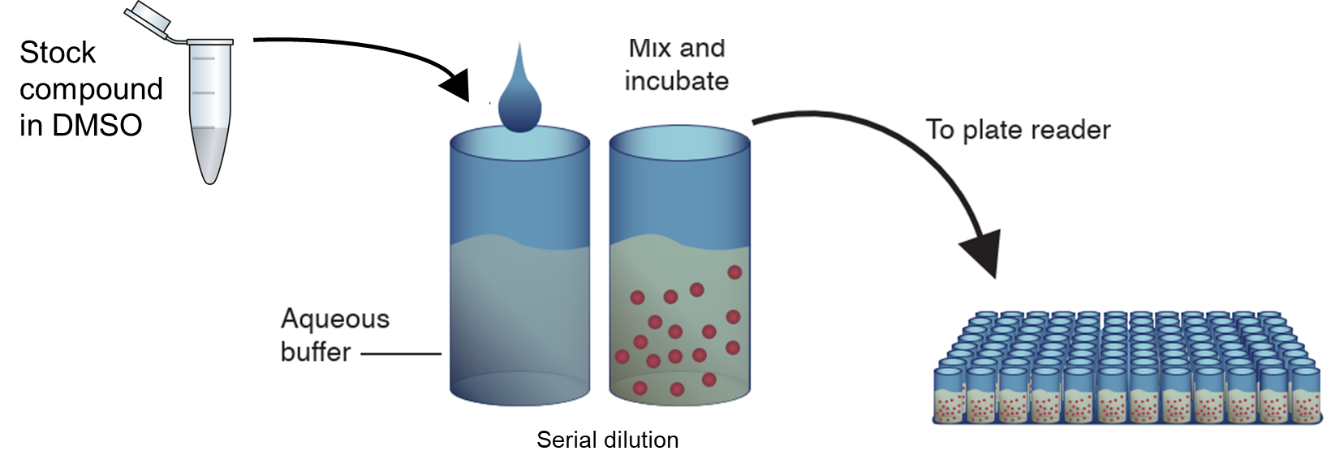
\includegraphics[width=1\linewidth]{media-01/image3} 

}

\caption{Kinetic solubility 측정법 모식도}\label{fig:01-03}
\end{figure}



이 때 약물의 침전을 검출하는 방법은 Nephelometry, Turbidimetry 그리고 Direct measurement가 있다 (표 \ref{tab:table01-05}).
약물을 여러 농도로 용매에 용해시켰을 때, 침전이 생기기 시작하는 농도부터 침전물에 의해 빛이 산란되는데, 이 변곡점을 확인하는 방법이 바로 Nephelometry이다.
반대로 침전이 생기기 시작하는 농도부터 침전물에 의해 빛의 투과가 감소하는데, 이 변곡점을 확인하는 방법이 Turbidimetry이다.
마지막으로 Direct measurement란 UV 흡광도와 약물 농도는 선형 비례 관계에 있음을 이용하여 측정된 UV 흡광도로부터 미지의 약물 농도를 정량하는 방법이다.

\begin{longtable}[]{@{}
  >{\raggedright\arraybackslash}p{(\columnwidth - 4\tabcolsep) * \real{0.3624}}
  >{\raggedright\arraybackslash}p{(\columnwidth - 4\tabcolsep) * \real{0.3691}}
  >{\raggedright\arraybackslash}p{(\columnwidth - 4\tabcolsep) * \real{0.2685}}@{}}
\caption{\label{tab:table01-05} Kinetic solubility의 침전을 검출하는 방법}\tabularnewline
\toprule()
\begin{minipage}[b]{\linewidth}\raggedright
Nephelometry
\end{minipage} & \begin{minipage}[b]{\linewidth}\raggedright
Turbidimetry
\end{minipage} & \begin{minipage}[b]{\linewidth}\raggedright
Direct measurement
\end{minipage} \\
\midrule()
\endfirsthead
\toprule()
\begin{minipage}[b]{\linewidth}\raggedright
Nephelometry
\end{minipage} & \begin{minipage}[b]{\linewidth}\raggedright
Turbidimetry
\end{minipage} & \begin{minipage}[b]{\linewidth}\raggedright
Direct measurement
\end{minipage} \\
\midrule()
\endhead
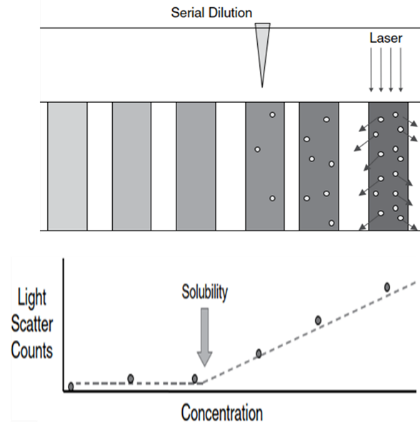
\includegraphics{./media-01/image4.png} & 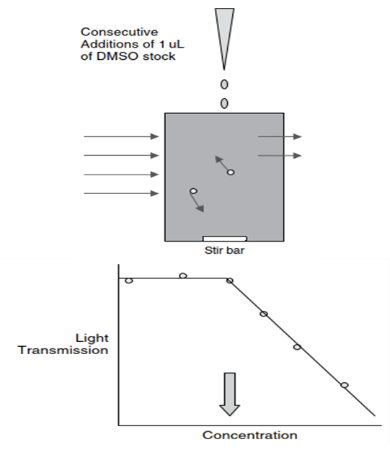
\includegraphics{./media-01/image5.png} & 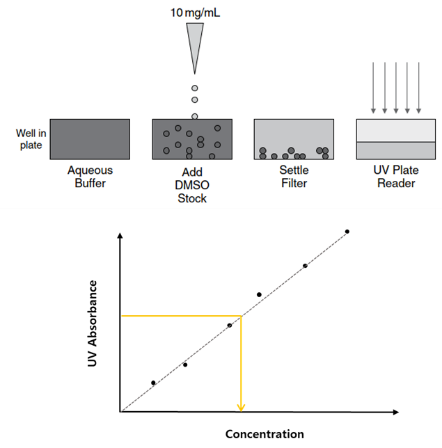
\includegraphics{./media-01/image6.png} \\
\bottomrule()
\end{longtable}

\hypertarget{thermodynamic-solubility}{%
\subsubsection{Thermodynamic solubility}\label{thermodynamic-solubility}}

Thermodynamic solubility는 과량의 결정성 고체 약물을 특정 수용매에 직접
첨가한 후, 평형상태에 도달했을 때 용해된 약물의 농도를 측정한다 (그림 \ref{fig:01-04}).
따라서 Thermodynamic solubility는 Equilibrium solubility라고도 한다.
용해도 측정 방법의 gold standard로 여겨 지고 있어, 주로 Drug development 단계에서 수행된다.
그러나 평형상태에 도달하기 위해서는 24시간 이상 충분히 반응시켜야 하므로 용해도 측정에 오랜 시간이 소요되며, 측정 시 많은 양의 약물이 필요하다.

\begin{figure}

{\centering 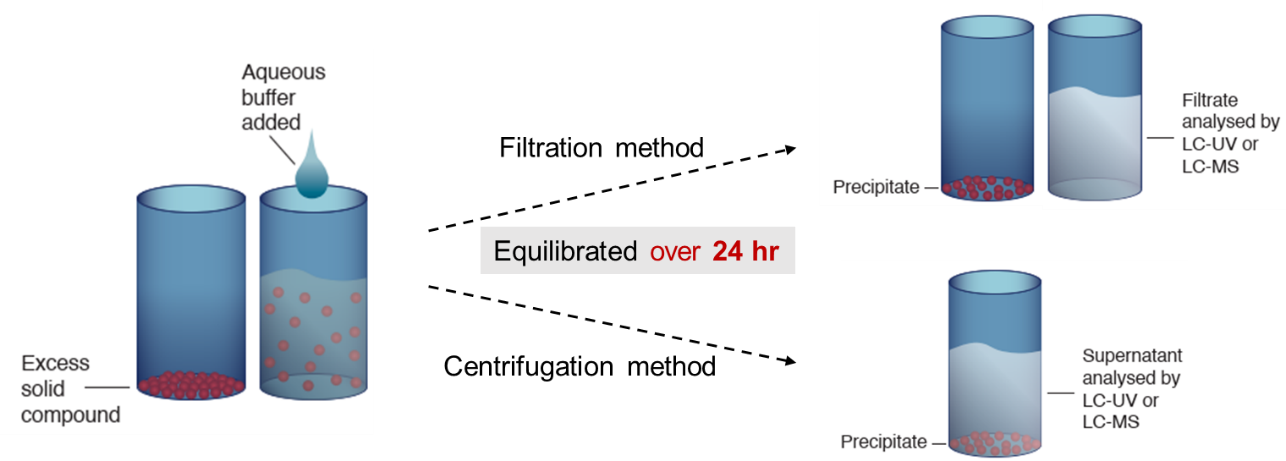
\includegraphics[width=1\linewidth]{media-01/image7} 

}

\caption{Thermodynamic solubility 측정법 모식도}\label{fig:01-04}
\end{figure}



Thermodynamic solubility의 경우 시간이 지날수록 용해된 약물의 농도가 증가하다가 평형상태에 도달하면 일정한 농도로 유지된다.
반면 Kinetic solubility는 약물이 녹아 있는 유기용매에 수용액을 첨가하면서 약물이 석출되기 시작하는 시점에 측정하므로, 시간이 지날수록 약물의 농도는 감소하는 양상을 보인다 (그림 \ref{fig:01-05}).

Thermodynamic solubility는 Kinetic solubility에 비해 낮은 용해도 값을 보이는 경우가 많은데, 이는 약물의 결정다형 (Polymorphism)이 결정형 (Crystal form)인 경우이다.
결정형인 약물일지라도 Kinetic solubility 측정 시 생기는 침전물은 무정형 (Amorphous form)인 경우가 많다.
그런데 용해도는 일반적으로 결정형보다 무정형이 높기 때문에 두 방법 사이에 용해도 차이가 발생하게 된다.

\begin{figure}

{\centering 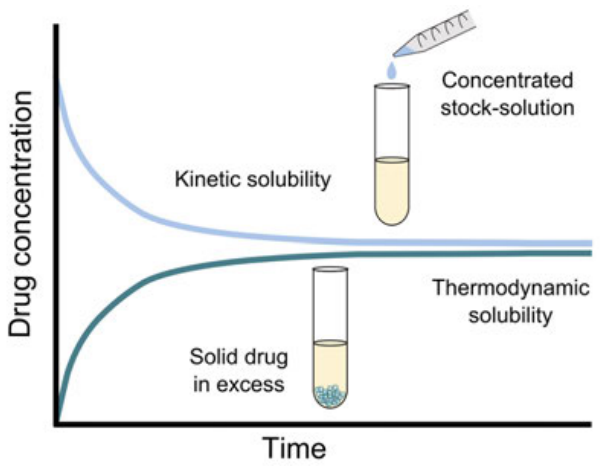
\includegraphics[width=1\linewidth]{media-01/image8} 

}

\caption{Kinetic solubility와 Thermodynamic solubility의 비교}\label{fig:01-05}
\end{figure}



\hypertarget{uxb9fauxc74cuxb9d0}{%
\section{맺음말}\label{uxb9fauxc74cuxb9d0}}

이상으로 ADME의 기초자료: Physicochemical properties에서 용해도에 대해 알아보았다.
용해도는 약물의 흡수 및 생체이용률에 영향을 주는 약물의 특성 중 하나로, in vitro/in vivo 평가 시 평가 농도 혹은 용량의 결정과 평가 결과에 영향을 미치기도 한다.
또한 여러 용매 조건에서의 용해도 측정 결과는 임상시험 혹은 품목허가 등을 위해서도 필수적으로 제출해야 하는 자료이기도 하다.
최근 많은 개발사들이 highly potent한 약물을 발굴하려 노력하면서, 화합물의 lipophilicity 또한 더욱 높아지는 경향을 보이고 있어 용해도의 중요성이 더욱 크게 여겨지고 있다.
따라서 수용액, 유기용매, pH별 buffer, compendial 및 bio-relevant media 등과 같은 다양한 용매 조건에서의 용해도 평가에 대하여 정확히 이해하고, 이를 적절히 활용하는 것이 중요하겠다.

\textbf{참고문헌}

(편집자: 이 참고문헌은 모두 인용 위치가 본문 내에서 구체적으로 표시되어야 합니다.)

\begin{enumerate}
\def\labelenumi{\arabic{enumi}.}
\tightlist
\item
  Edward H. Kerns and Li Di, Drug-like properties: Concepts, Structure Design and Methods.
\item
  Lubrizol Life Science, Biopharmaceutical Classification System, 2019 \url{https://3ehzg6104228bwtte1se19g6-wpengine.netdna-ssl.com/wp-content/uploads/2019/10/TB-28-Biopharmaceutical-Classification-System.pdf}
\item
  Everything you need to know about ADME, 3rd Edition, Cyprotex
\item
  Alskär, L. C. et al., Improved molecular understanding of lipid-based formulations, Digital Comprehensive Summaries of Uppsala Dissertations from the Faculty of Pharmacy 262, 2018.
\item
  Eleni Rinaki et al., Pharmaceutical Research, 20(12), 2003.
\item
  Sandra Klein et al., The AAPS Journal, 12(3), 2010.
\item
  Mark G. Papich and Marilyn N. Martinez, The AAPS Journal, 2015.
\item
  Edward H. Kerns et al., Current Drug Metabolism, 9, 879-885, 2008.
\item
  M9 Biopharmaceutics classification system based biowaivers, 2018.
\item
  Jochen Maas et al., European Journal of Pharmaceutics and Biopharmaceutics, 66, 1-10, 2007.
\item
  Prachi Shekhawat and Varsha Pokharkar, Acta Pharmaceutica Sinica B, 2016.
\end{enumerate}

\hypertarget{uxd22cuxacfcuxb3c4}{%
\chapter{투과도}\label{uxd22cuxacfcuxb3c4}}

\Large\hfill

신초롱
\normalsize

\hypertarget{uxc11cuxb860-1}{%
\section{서론}\label{uxc11cuxb860-1}}

투과도 (Permeability)란 물질이 세포막을 통하여 수송되는 속도로서 정의된다.
경구 투여된 약물이 전신순환혈로 도달, 즉 흡수되기 위해서는 약물이 소화관 점막 상피세포막을 투과하는 과정을 반드시 거쳐야만 한다.
위, 소장, 간을 거쳐 전신으로 흡수된 약물은 타겟 조직으로 도달한 후 체외로 배설되기까지 여러 이행 과정을 거치게 되는데, 이 때도 여러 생체막의 관문을 통과하게 된다.
따라서 투과도는 흡수, 분포, 대사, 배설 과정 전반에 걸쳐 영향을 주는 인자로서 약동학의 가장 기초적인 자료라 할 수 있다 (그림 \ref{fig:02-01}).

\begin{figure}

{\centering 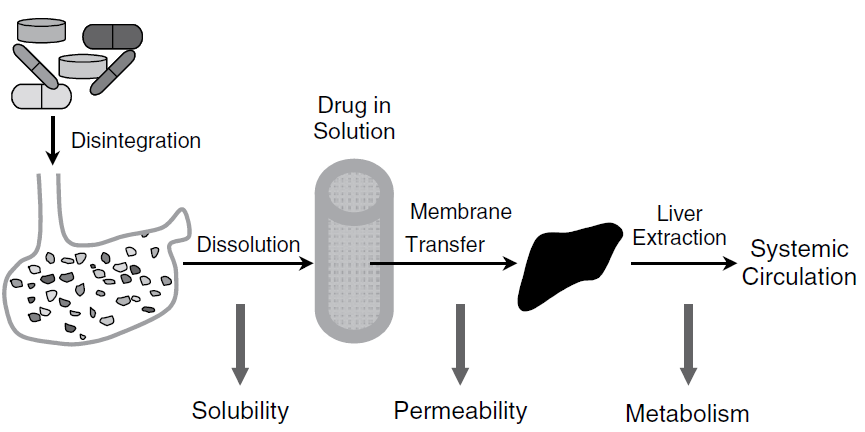
\includegraphics[width=1\linewidth]{media-01/image1} 

}

\caption{생체막의 종류 및 관련 인자}\label{fig:02-01}
\end{figure}



이 장에서는 투과도의 개념과 막 투과 기전을 자세히 기술하고, 대표적인 투과도 평가 시험의 특성을 비교하여 실제 신약 개발 과정에서 목적에 맞는 시험을 설계하고 결과를 적절히 해석 및 활용할 수 있도록 돕고자 한다.

\hypertarget{uxae30uxbcf8-uxac1cuxb150}{%
\section{기본 개념}\label{uxae30uxbcf8-uxac1cuxb150}}

\hypertarget{uxb9c9-uxd22cuxacfc-uxae30uxc804}{%
\subsection{막 투과 기전}\label{uxb9c9-uxd22cuxacfc-uxae30uxc804}}

생체막은 단백질을 함유한 인지질 이중층 (phospholipid bilayer)으로 구성되어 있으며, 인지질 분자의 소수성 꼬리는 내측으로, 친수성 머리는 세포질 및 세포 외부로 향하도록 구성되어 있다 (그림 \ref{fig:02-02}).

\begin{figure}

{\centering 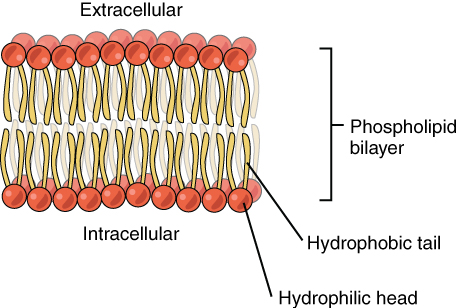
\includegraphics[width=1\linewidth]{media-02/image2} 

}

\caption{생체막의 구조: 인지질 이중층}\label{fig:02-02}
\end{figure}



막 투과 기전을 이해하기 위하여 경구 투여된 약물이 장 상피세포를 투과하여 혈액으로 들어가는 과정을 생각해보자.
약물이 점막 상피세포의 brush border막을 통과하여 세포 내로 유입되고, 세포 내 확산 이동한 다음 측저막 (basolateral membrane)을 투과하여 모세혈관에 도달한다.
이러한 transcellular 수송은 막 내외의 농도 구배에 따른 수동수송 (passive transport) 뿐만 아니라 담체 (carrier), 펌프, 채널 등과 같은 막 단백질이 관여하여 농도 구배에 역행하는 능동수송 (active transport) 방식에 의해서도 이루어진다.
반면 세포 간극 (tight junction)을 통과하는 paracellular 수송은 수동수송 방식으로만 행하여진다 (그림 \ref{fig:02-03}).
수동수송과 능동수송의 차이는 생체 대사에너지에 대한 의존성으로, 후자는 수송 시 생체 대사에너지를 필요로 한다.
따라서 능동수송의 경우 대사 저해제 혹은 저온 환경에 의해 대사가 억제되면 투과도가 낮아질 수 있으며, 관여하는 막 단백질의 양에 한계가 있어 투과도의 포화 현상이 나타날 수 있다.

\begin{figure}

{\centering 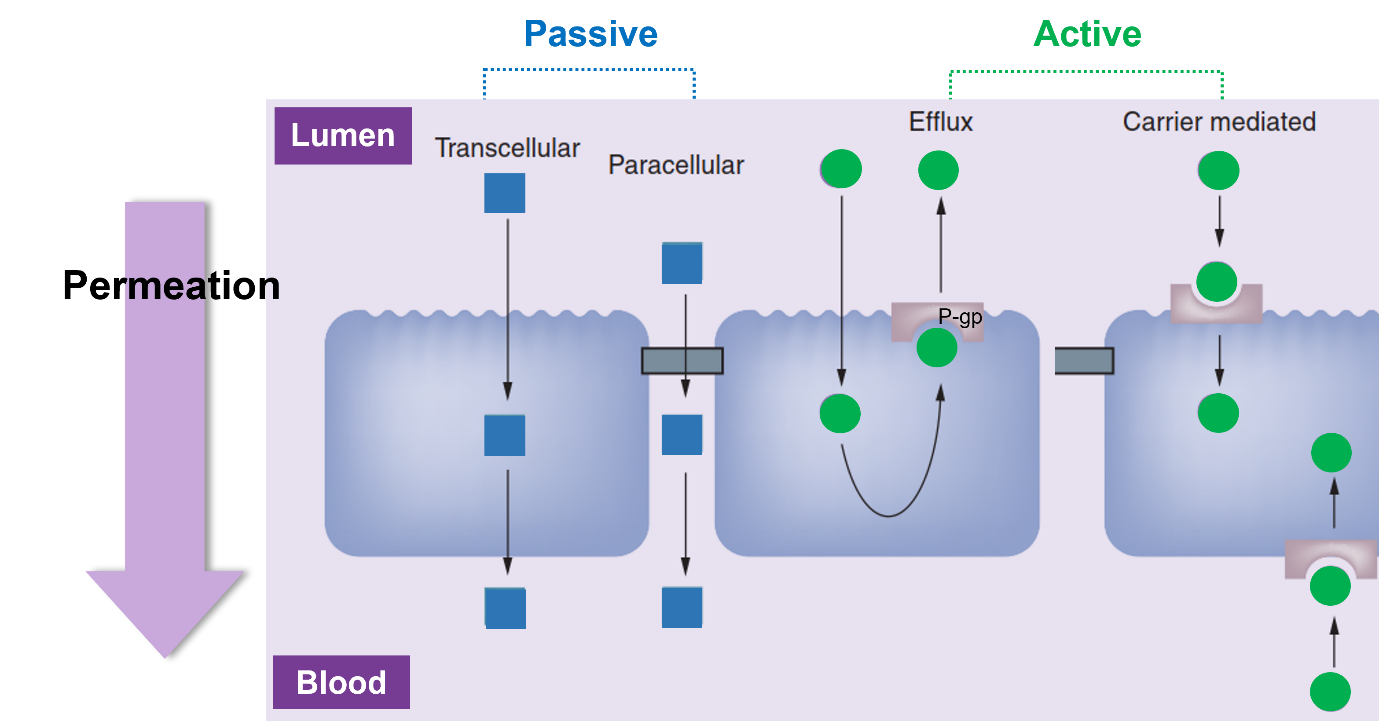
\includegraphics[width=1\linewidth]{media-02/image3} 

}

\caption{막 투과 기전}\label{fig:02-03}
\end{figure}



\hypertarget{uxd22cuxacfcuxb3c4uxc5d0-uxc601uxd5a5uxc744-uxc8fcuxb294-uxc778uxc790}{%
\subsection{투과도에 영향을 주는 인자}\label{uxd22cuxacfcuxb3c4uxc5d0-uxc601uxd5a5uxc744-uxc8fcuxb294-uxc778uxc790}}

앞서 살펴본 바와 같이 생체막은 인지질 이중층으로 구성되어 있어 약물의 지용성이 높을수록 세포막을 투과하기 쉽다.
그리고 해리형에 비해 비해리형은 지용성이 높으므로 더욱 잘 투과할 수 있으며, 따라서 약물의 pKa 및 막 내외의 pH 조건에 따라 투과도가 결정될 수 있다.
또한 soluble한 약물만이 투과할 수 있기에 약물의 용해도 역시 투과도에 영향을 주는 요인이다.
막 단백질과의 상호작용 또한 약물의 투과도를 결정하는 인자로, 가장 대표적인 예로서 uptake 혹은 efflux transporter의 발현 정도 및 그에 대한 약물의 친화도 (affinity)에 의해 약물의 투과도가 결정되기도 한다 (그림 \ref{fig:02-04}).

높은 투과도를 보이는 약물의 특성을 요약하면 다음과 같다.

\begin{itemize}
\tightlist
\item
  High lipophilicity
\item
  Low ionizability
\item
  High solubility
\item
  High affinity to the uptake transporters
\item
  Low affinity to the efflux transporters
\end{itemize}

\begin{figure}

{\centering 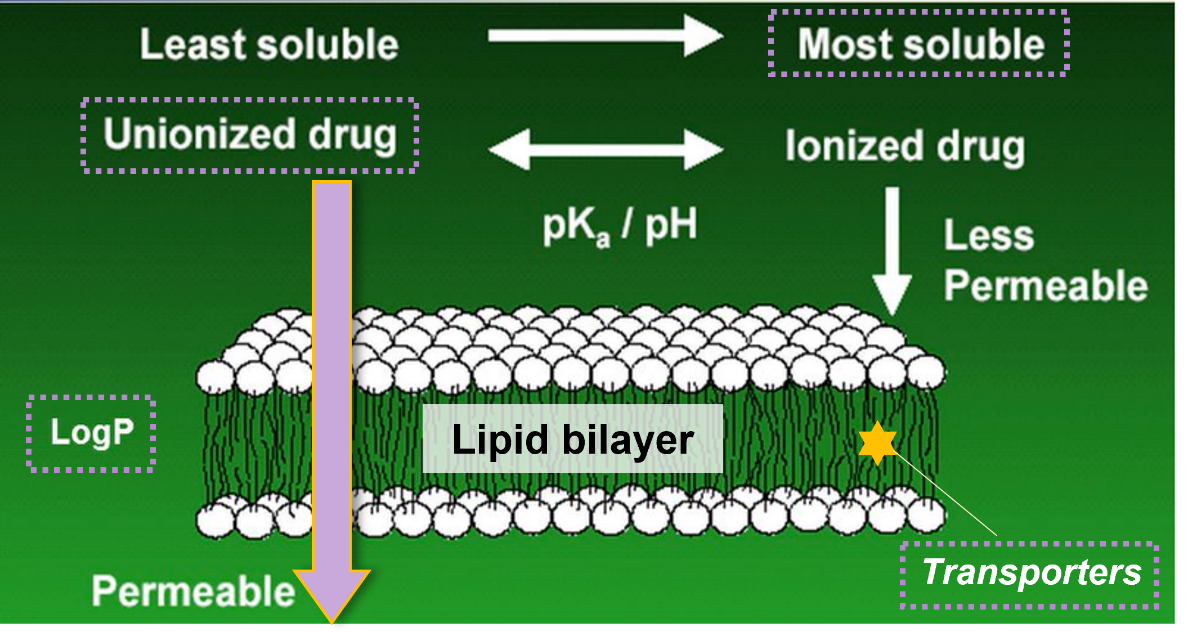
\includegraphics[width=1\linewidth]{media-02/image4} 

}

\caption{약물의 투과도에 영향을 주는 인자}\label{fig:02-04}
\end{figure}



\hypertarget{uxd22cuxacfcuxb3c4-uxd3c9uxac00-uxc2dcuxd5d8}{%
\section{투과도 평가 시험}\label{uxd22cuxacfcuxb3c4-uxd3c9uxac00-uxc2dcuxd5d8}}

\hypertarget{pampa-parallel-artificial-membrane-permeability-assay}{%
\subsection{PAMPA (Parallel Artificial Membrane Permeability Assay)}\label{pampa-parallel-artificial-membrane-permeability-assay}}

인공지질막을 이용한 시험법으로, 여러 막 투과 기전 중 수동수송에 대한 평가만이 가능하다는 특징이 있다.
주된 흡수 장기인 소장에서 약물은 주로 수동수송에 의해 장 상피세포를 투과하는 것으로 알려져 있으며, 이에 신약 개발 초기 단계에서 다수의 화합물에 대하여 빠르게 투과도를 평가하기 위하여 PAMPA 시험법이 널리 활용되고 있다.

PAMPA 시험은 그림 \ref{fig:02-05}와 같이 인공지질막이 있는 Kit를 사용하여 평가한다.

\begin{figure}

{\centering 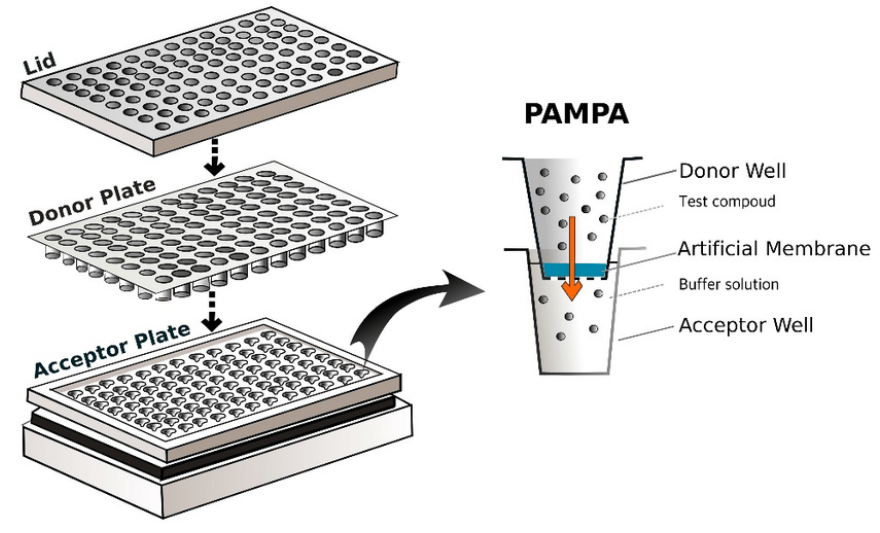
\includegraphics[width=1\linewidth]{media-02/image5} 

}

\caption{PAMPA 시험의 모식도}\label{fig:02-05}
\end{figure}



먼저 DMSO 등의 유기용매에 약물을 완전히 용해시켜 stock solution을 만든다.
그리고 Donor plate의 well에는 약물을 평가하고자 하는 농도가 되도록 PBS buffer를 이용해 희석한 후 넣고, Acceptor plate의 well에는 PBS buffer를 넣어 25 ˚C에서 5시간 이상 배양한 후 Donor 및 Acceptor plate에서의 약물 농도를 LC-MS/MS와 같은 분석 기기로 측정하여 아래와 같은 식으로 P\textsubscript{e}값을 산출한다.

\begin{equation}
P_{e} = C\  \times \left\lbrack - Ln\mspace{6mu}\left( 1 - \frac{\lbrack drug\rbrack_{acceptor}}{\lbrack drug\rbrack_{equilibrium}} \right) \right\rbrack
\label{eq:eq02-01} 
\end{equation}

{[}drug{]}\textsubscript{equilibrium} = {[}drug{]}\textsubscript{donor} V\textsubscript{D} + {[}drug{]}\textsubscript{acceptor} x V\textsubscript{A} / (V\textsubscript{D} + V\textsubscript{A})\\
C = V\textsubscript{D} × V\textsubscript{A} / (V\textsubscript{D} + V\textsubscript{A}) × t × A\\
V\textsubscript{D} = volume of donor compartment\\
V\textsubscript{A} = volume of acceptor compartment\\
A = filter area\\
t = incubation time (in seconds)\\
{[}drug{]}\textsubscript{acceptor} = Concentration of compound in the acceptor compartment at the assay completion\\
{[}drug{]}\textsubscript{donor} = Concentration of compound in the donor compartment at the assay completion\\
{[}drug{]}\textsubscript{equilibrium} = Concentration of compound at theoretical equilibrium

별도의 세포 배양 과정이 필요 없고, 약물의 농도를 UV plate reader를 활용하여 측정할 경우 대량의 화합물을 빠르게 평가할 수 있다는 것이 PAMPA의 가장 큰 장점이라 할 수 있다.
또한 세포주를 이용한 시험법 (cell-based assay)과 비교하였을 때 더욱 넓은 pH 범위에서 평가가 가능하므로, 보다 다양한 막 투과도 평가에 활용되고 있다.
그 예로 PAMPA-BBB를 활용하여 Brain-Blood Barrier에 대한 약물의 투과도를 평가할 수 있다.
그러나, 만약 UV plate reader를 활용하는 경우 약물의 평가 농도가 비교적 고농도에서 수행되어야 하는데, 이 때 용해도가 매우 낮은 약물인 경우 시험이 불가능할 수 있다.
그리고 수동수송 방식만이 구현되어 있어 실제로 약물이 막을 투과하는 기전을 완전히 재현하지는 못한 시험계로서 특히 transporter와 약물 간 상호작용을 평가할 수 없다는 단점이 있다.

\hypertarget{caco-2-cell-based-permeability-assay}{%
\subsection{Caco-2 cell-based permeability assay}\label{caco-2-cell-based-permeability-assay}}

사람 대장암 세포에서 유래한 Caco-2 세포주를 이용한 시험법으로, Caco-2
세포는 분화되면서 형태학적 및 기능학적으로 사람의 소장 상피세포와 유사한
특성 (예: microvilli을 가지며 tight junction을 형성)을 보이므로 경구용
약물의 투과도 평가 시 많이 활용되고 있다.

Caco-2 투과도 시험은 그림 \ref{fig:02-06}에 나타낸 바와 같이, well plate에
monolayer로 Caco-2 세포를 배양하고, Apical 및 Basolateral side에 각각
약물을 처리한 후 약물의 양방향성 수송능을 측정하기 위하여 Apical 및
Basolateral side 모두에서 약물 농도를 측정한다.

\begin{figure}

{\centering 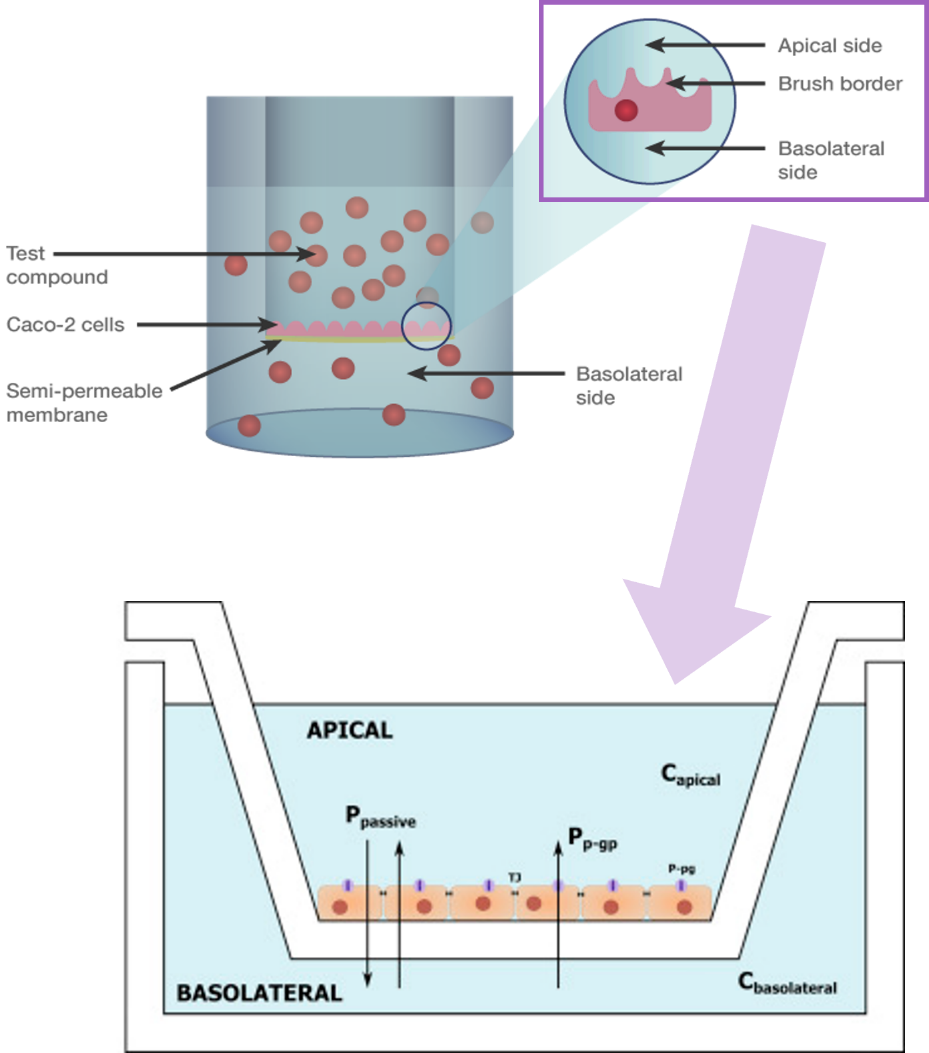
\includegraphics[width=1\linewidth]{media-02/image6} 

}

\caption{Caco-2 cell-based permeability assay 방법}\label{fig:02-06}
\end{figure}



그리고 아래와 같은 식을 이용하여 세포막 투과 계수 (P\textsubscript{app}, Apparent permeability coefficient) 및 Efflux ratio를 산출한다.

\begin{equation}
P_{app} = \frac{\frac{dQ}{dt}}{A \cdot C_0} \\
Efflux\ ratio = \frac{P_{app (B to A)}}{P_{app (A to B)}}
\label{eq:eq02-02} 
\end{equation}

여기서 dQ/dt는 초기 약물 수송 속도 (initial transport rate, μmol/s), A는 well의 표면적 (the surface area of the monolayer, cm\textsuperscript{2}), C\textsubscript{0}는 처리한 약물의 농도 (initial concentration in the donor chamber, μmol/cm\textsuperscript{3})를 의미한다.

Caco-2 투과도 시험계에서는 약물의 수동수송 뿐만 아니라 능동수송 방식에 의한 막 투과도 행하여 지며, 내강막 (Apical membrane) 및 측저막 (Basolateral membrane) 간 양방향의 수송이 모두 일어난다. 또한 장에 많이 발현되어 있으며 약물의 흡수를 저해하는 P-glycoprotein (P-gp) 및 Breast cancer resistant protein (BCRP)와 같은 efflux transporter의 기질성 여부까지 판단할 수 있다 (기질인 경우 Efflux ratio \textgreater{} 2). 그러나 세포 배양 시 3주 이상이 소요되고, 시험 1주일 전 antibiotics-free media로 배양하는 과정 중 contamination의 가능성도 있으며 시험 수행에 숙련된 기술이 필요하기 때문에 수행자나 기관에 따라 그 값의 편차가 심하다는 단점이 있다. 또한 Caco-2 세포주가 사람의 대장세포라 실제 약물의 흡수가 많이 이루어지는 소장과는 다소 차이가 있을 수 있다.

\hypertarget{mdck-cell-based-permeability-assay}{%
\subsection{MDCK cell-based permeability assay}\label{mdck-cell-based-permeability-assay}}

개의 신장에서 유래한 MDCK (Madin-Darby Canine Kidney) 세포주를 이용한 시험법으로, 소장 상피세포의 tight junction과 유사한 구조의 cell monolayer에서 약물의 투과도를 평가한다. Caco-2와 마찬가지로 모든 투과 기전이 반영된 시험계로서, efflux transporter에 대한 기질성을 평가할 수 있다. 시험방법은 Caco-2 세포주를 이용하는 방법과 유사하지만, 일반적으로 3\textasciitilde4일을 배양하면 cell monolayer가 형성되므로 보다 신속히 평가를 진행할 수 있다. 다만 내재된 transporter의 발현 수준이 낮아 특정 transporter가 과발현 되도록 만들어진 형질전환 세포주 (transfected cell line)의 형태로 많이 사용된다. 따라서 약물의 세포막 투과도 평가 외에도 여러 transporter에 대한 기질성 및 저해능 평가 시험에도 많이 활용되고 있다 (예: MDCK II-MDR1 cell line).

\begin{figure}

{\centering 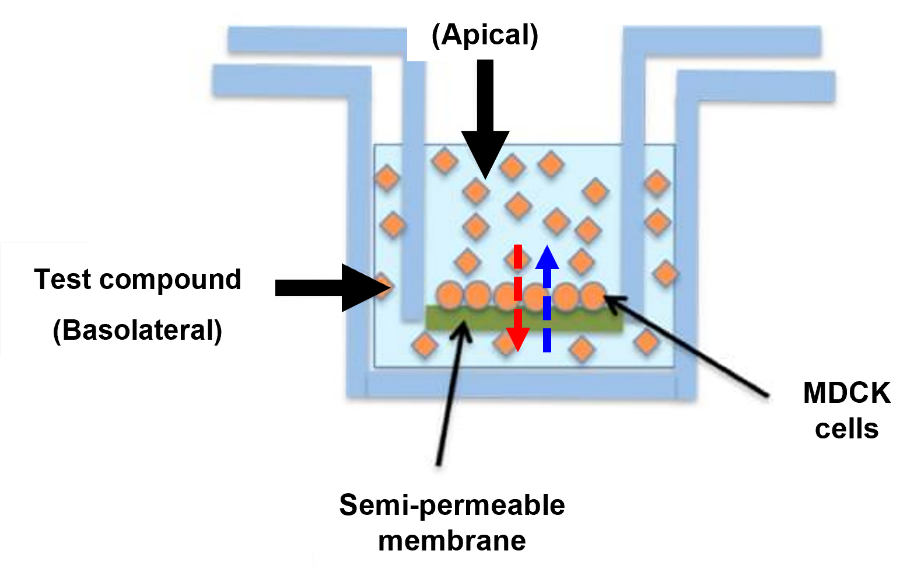
\includegraphics[width=1\linewidth]{media-02/image7} 

}

\caption{MDCK cell-based permeability assay}\label{fig:02-07}
\end{figure}



\begin{longtable}[]{@{}
  >{\raggedright\arraybackslash}p{(\columnwidth - 6\tabcolsep) * \real{0.2917}}
  >{\raggedright\arraybackslash}p{(\columnwidth - 6\tabcolsep) * \real{0.2222}}
  >{\raggedright\arraybackslash}p{(\columnwidth - 6\tabcolsep) * \real{0.2222}}
  >{\raggedright\arraybackslash}p{(\columnwidth - 6\tabcolsep) * \real{0.2222}}@{}}
\caption{\label{tab:table02-01} 투과도 평가 시험 방법 별 특성 비교}\tabularnewline
\toprule()
\begin{minipage}[b]{\linewidth}\raggedright
\end{minipage} & \begin{minipage}[b]{\linewidth}\raggedright
\textbf{PAMPA}
\end{minipage} & \begin{minipage}[b]{\linewidth}\raggedright
\textbf{Caco-2
cell-based}
\end{minipage} & \begin{minipage}[b]{\linewidth}\raggedright
\textbf{MDCK
cell-based}
\end{minipage} \\
\midrule()
\endfirsthead
\toprule()
\begin{minipage}[b]{\linewidth}\raggedright
\end{minipage} & \begin{minipage}[b]{\linewidth}\raggedright
\textbf{PAMPA}
\end{minipage} & \begin{minipage}[b]{\linewidth}\raggedright
\textbf{Caco-2
cell-based}
\end{minipage} & \begin{minipage}[b]{\linewidth}\raggedright
\textbf{MDCK
cell-based}
\end{minipage} \\
\midrule()
\endhead
\textbf{Cell origin} & Artificial
membrane & Human
colorectal
carcinoma
cells & Madin-Darby
canine kidney
strain cells \\
\textbf{Cell
morphology} & - & Intestinal
epithelium & Distal tubule
epithelium \\
\textbf{Cell growing
time} & - & \textgreater{} 21 days & 3\textasciitilde4 days \\
\textbf{Permeation
mechanisms} & Passive
diffusion & Passive
diffusion,
Active
transport,

Paracellular
and Efflux & \\
\textbf{Direction of
transport} & One-way

(Donor →
Acceptor) & B
i-directional

(Apical ↔
Basolateral) & \\
\textbf{Expression of
transporters} & & & \\
\textbf{Uptake
transporters} & Not expressed & OATP1B1,
OATP1B3,
OATP2B1,
PepT1, OCT1,
OCT2 and OCT3 & OCT2, peptide
and
m
onocarboxylic
acids \\
\textbf{Efflux
transporters} & Not expressed & P-gp (MDR1),
MRP2,

MRP4 and BCRP & P-gp (MDR1),
MRP1,

MRP2 and MRP5 \\
\textbf{Metabolism} & No & Yes & Yes \\
\bottomrule()
\end{longtable}

-: not applicable.

\hypertarget{uxd22cuxacfcuxb3c4-uxd3c9uxac00-uxacb0uxacfcuxc758-uxd574uxc11d-uxbc0f-uxd65cuxc6a9}{%
\section{투과도 평가 결과의 해석 및 활용}\label{uxd22cuxacfcuxb3c4-uxd3c9uxac00-uxacb0uxacfcuxc758-uxd574uxc11d-uxbc0f-uxd65cuxc6a9}}

앞서 설명한 \emph{in vitro} 시험들을 통해 약물의 세포막 투과 계수를 산출할 수 있으며, 이를 토대로 그 약물의 소장에서의 흡수 정도를 예측하게 된다. 또한 \emph{in vitro} 활성 시험에 있어서도 화합물이 세포 내 표적에 도달하여 약리 작용을 나타내기 위해서는 먼저 생체막을 투과해야 한다. 따라서 대다수의 제약사에서는 초기의 신약 탐색 단계 (drug discovery)부터 투과도 시험을 수행하여 후보물질을 선별하고 있다.

특히 Caco-2 세포주를 이용한 약물의 투과도는 사람의 소장 내 약물의 흡수율과 높은 상관성을 보이는 것으로 보고되어 있다 (그림 \ref{fig:02-08}). FDA의 `생물약제학적 분류체계 (Biopharmaceutics Classification System, BCS)' 가이드라인\textsuperscript{6}에 따르면, 약물의 용해도 및 장관 투과도에 근거하여 약물 성분을 분류하기 위해서는 약물의 세포막 투과 계수가 필요한데 이 때 사람에서 유래한 Caco-2 세포주를 이용한 약물의 투과도 평가 결과를 활용하도록 권고하고 있다. 또한 Caco-2 세포주를 이용한 약물의 투과도는 사람의 흡수속도상수 (absorption rate constant, \emph{k}\textsubscript{a})를 예측하는 데에도 활용될 수 있다.

\begin{figure}

{\centering 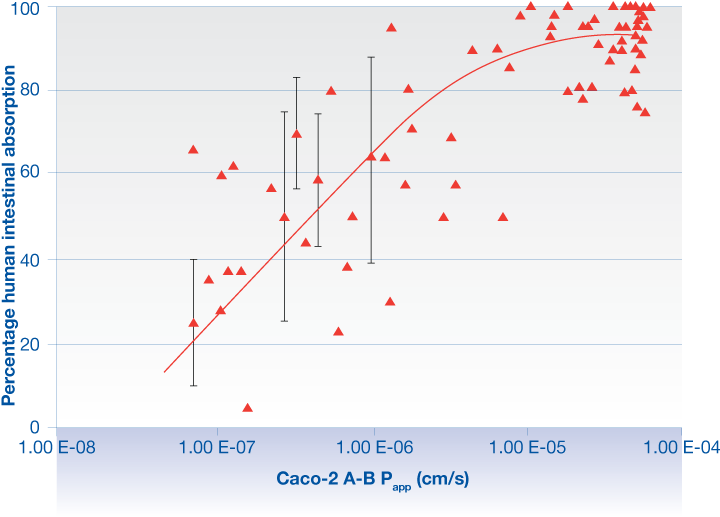
\includegraphics[width=1\linewidth]{media-02/image8} 

}

\caption{Caco-2 투과도와 사람 소장 흡수율 간의 상관 관계}\label{fig:02-08}
\end{figure}



PAMPA 시험의 경우 투과도 결과를 해석하기 위한 절대적인 기준은 없으며 시험기관 혹은 시험자마다 상이하다. 실무에서 흔히 사용되는 기준을 소개하면, PAMPA 시험 결과 투과 계수 (P\textsubscript{e})가 10*10\textsuperscript{-6} cm/sec 이상이면 투과도가 높은 약물로 분류하는 경우가 많다. 그러나 P\textsubscript{e} 값이 10*10\textsuperscript{-6} cm/sec 이하인 경우라 할지라도 경구용 약물로 개발이 불가한 것은 아니며, 1*10\textsuperscript{-6} cm/sec 이상의 약물이면 경구용 약물로 개발 가능한 수준으로 판단하는 경우도 있다.

Caco-2 시험에서 산출된 Apical to Basolateral 방향의 겉보기 투과계수 (P\textsubscript{app,} A to B)는 동일한 시험 배치에서 평가한 기준 약물 (reference drug)의 결과를 기반으로 시험 약물의 투과도가 높거나 중간 수준 혹은 낮다고 분류한다. 여기서 기준 약물이란 위에서 언급한 FDA의 가이드라인에 명시되어 있는 약물로서, 사람 소장에서의 흡수 분율 (fraction of human intestinal absorption; f\textsubscript{a})에 따라 high (≥85\%), moderate (50 - 84\%), low (\textless50\%) 및 zero-permeable 약물로 분류되어 있다. 보다 정확한 결과 해석을 위해서는 시험 약물과 더불어 high 및 low-permeable 기준 약물을 1종씩 선택하여 함께 평가를 수행하는 것이 바람직하다. 그리고 앞서 언급했지만, 세포주를 이용한 투과도 평가 시 efflux ratio가 2 이상이면 시험 약물이 해당 세포주에 발현된 efflux transporter의 기질성이 있다고 판단한다.

시험약물이 어떤 efflux transporter의 기질인지를 판단하려면, 평가하고자 하는 transporter의 알려진 기질 및 저해제를 처리하였을 때 시험 약물의 투과도 평가 결과가 어떻게 나타나는지를 확인하여야 한다. 다음 표 \ref{tab:caco-2-pgp}의 예시와 같이, P-gp에 대한 기질성을 판단하기 위해서는 P-gp의 기질인 Talinolol과 저해제인 Verapamil 등을 이용하여 투과도 시험을 수행하여야 한다. 평가 결과를 보면 Test drug A는 알려진 P-gp의 기질인 Talinolol과 유사한 결과를 나타내었다. 즉 efflux ratio가 2 이상이면서 저해제인 Verapamil을 함께 처리 시 apical to basolateral 방향의 P\textsubscript{app} 값이 2배 이상 증가한 것을 확인할 수 있다. 그 결과 저해제를 처리한 경우의 efflux ratio가 44.4로서 처리하지 않았을 때보다 2배 이상 감소하였다. 따라서 Test drug A는 P-gp의 기질인 것으로 판단된다. 반면 Test drug B는 efflux ratio가 모두 2 이하이고, 저해제 처리 유무에 따라 P\textsubscript{app} 및 efflux ratio가 변하지 않고 일정한 값으로 산출되었다. 그러므로 Test drug B는 P-gp의 기질이 아니며, P-gp 외 Caco-2 세포주에 발현된 다른 efflux transporter의 기질도 아닌 것으로 해석된다.



\begin{table}

\caption{\label{tab:caco-2-pgp}Caco-2 세포주를 이용한 P-gp 기질성 평가 예시}
\centering
\begin{tabular}[t]{lllllll}
\toprule
\multicolumn{1}{c}{ } & \multicolumn{3}{c}{Without Verapamil (P-gp inhibitor)} & \multicolumn{3}{c}{With Verapamil (P-gp inhibitor)} \\
\cmidrule(l{3pt}r{3pt}){2-4} \cmidrule(l{3pt}r{3pt}){5-7}
Compound & Papp (A to B) [x10-6 cm/sec] & Papp (B to A) [x10-6 cm/sec] & Efflux ratio & Papp (A to B) [x10-6 cm/sec]  & Papp (B to A) [x10-6 cm/sec]  & Efflux ratio \\
\midrule
Talinolol (P-gp substrate) & 0.292 & 11.5 & 39.3 & 1.07 & 1.34 & 1.25\\
Test drug A & 0.397 & 40.1 & 101 & 0.959 & 42.6 & 44.4\\
Test drug B & 12.6 & 22.5 & 1.78 & 11.8 & 24.3 & 2.05\\
\bottomrule
\end{tabular}
\end{table}

P\textsubscript{app} (A to B): permeability coefficient in apical to basolateral direction, P\textsubscript{app} (B to A): permeability coefficient in basolateral to apical direction.

\hypertarget{uxd22cuxacfcuxb3c4-uxd3c9uxac00-uxc2dc-uxace0uxb824uxc0acuxd56d} \right) = \frac{total\ compound\ in\ both\ of\ A/B\ sides\ at\ the\ end\ of\ experiment\ (nmol)}{initial\ compound\ present\ (nmol)}\  \times \ 100 \\
A:\ apical,\ B:\ basolateral
\label{eq:eq02-03}
\end{equation}

만약 어떤 약물의 투과도를 평가하였을 때 배양액 내 약물의 농도가 낮아서 low-permeable한 약물로 분류되었으나 동시에 회수율이 매우 낮다면, 결과를 해석함에 있어 정말 약물의 투과도가 낮았던 것인지 혹은 다른 원인에 의해 약물이 소실되어 배양액 내 잔존하지 않았던 것인지를 구별하기 어렵다.
따라서 적어도 75\% 이상의 회수율이 확인되어야 해당 시험계에서 산출된 투과도 값에 신뢰성이 있다고 판단할 수 있으며, 회수율이 낮은 경우 그 원인으로는 다음과 같은 사항이 포함된다.

\begin{itemize}
\tightlist
\item
  Non-specific binding of test compound to plastic material
\item
  Poor solubility of test compound in the media
\item
  Instability of test compound in the media (\emph{i.e.}, due to the metabolism in cell)
\item
  Accumulation of test compound in the cell monolayer
\end{itemize}

이 중 배양액 내 약물이 실험 제품의 plastic ware에 비특이적 결합(non-specific binding)을 하는 경우에는 배양액에 bovine serum을 첨가하여 약물이 plastic 대신 bovine serum과 결합하도록 한 다음 약물을 추출하거나 혹은 plastic material과 비특이적으로 결합한 약물을 유기용매로 wash out하여 추출하여 그 농도를 분석함으로써 낮은 회수율을 개선시키는 방법이 있다.

\hypertarget{uxb9fauxc74cuxb9d0-1}{%
\section{맺음말}\label{uxb9fauxc74cuxb9d0-1}}

이상으로 ADME의 기초자료: physicochemical properties에서 투과도에 대해 알아보았다.
투과도는 약물의 흡수와 관련된 주요 인자 중 하나이므로, 신약 개발 초기의 후보물질 탐색 시 물질 스크리닝을 위한 평가 항목으로 여겨진다.
그 외에도 사람에서의 약물 흡수를 예측하거나 efflux transporter와의 상호작용 연구 시 활용될 수 있다.
앞서 설명한 바와 같이 투과도를 평가하기 위한 \emph{in vitro} 시험은 다양하므로, 각 시험의 특성을 이해하고 평가하고자 하는 목적, 개발 단계 등에 따라 적절한 시험을 선택하여야 하겠다.
뿐만 아니라 원하는 결과를 얻을 수 있도록 시험을 잘 설계하고, 데이터를 정확히 해석하는 것 역시 중요하다.

\textbf{참고문헌}

(편집자: 이 참고문헌은 모두 인용 위치가 본문 내에서 구체적으로 표시되어야 합니다.)

\begin{enumerate}
\def\labelenumi{\arabic{enumi}.}
\tightlist
\item
  가톨릭대학교 계량약리학연구소. 신약개발을 위한 실전 약동학 I (2021).
\item
  약제학분과회. 생물약제학과 약물속도론: 약제학총서 3 (2005).
\item
  Di, Li, and Edward Kerns. \emph{Drug-like properties: concepts, structure design and methods from ADME to toxicity optimization}. Academic press (2015).
\item
  Cyprotex Ltd.~Everything you need to know about ADME, 3\textsuperscript{rd} Edition (2017).
\item
  Volpe, Donna A. "Drug-permeability and transporter assays in Caco-2 and MDCK cell lines." \emph{Future medicinal chemistry} 3.16 (2011): 2063-2077.
\item
  ICH Harmonised Guideline, M9 Biopharmaceutics Classification System-Based Biowaivers (2018).
\item
  Saxena, Amrita, et al.~"Pharmacokinetics, dose proportionality and permeability of S002-333 and its enantiomers, a potent antithrombotic agent, in rabbits." \emph{Xenobiotica} 45.11 (2015): 1016-1023.
\item
  Masungi, C., et al.~"Parallel artificial membrane permeability assay (PAMPA) combined with a 10-day multiscreen Caco-2 cell culture as a tool for assessing new drug candidates." \emph{Die Pharmazie-An International Journal of Pharmaceutical Sciences} 63.3 (2008): 194-199.
\end{enumerate}

\hypertarget{uxd608uxc7a5uxb2e8uxbc31uxacb0uxd569}{%
\chapter{혈장단백결합}\label{uxd608uxc7a5uxb2e8uxbc31uxacb0uxd569}}

\Large\hfill

원상범
\normalsize

\hypertarget{uxc11cuxb860-2}{%
\section{서론}\label{uxc11cuxb860-2}}

약을 복용하게 되면 위장관에서 붕해 및 용해되어 전신순환혈에 도달하는 흡수과정을 거치게 되고, 전신순환혈에 도달한 약물은 혈장 내 단백질과 결합하거나 유리된 상태로 존재하게 된다.
혈장 내 유리 상태의 약물은 생체막을 통과하여 신장이나 간 등 약물이 작용하는 여러 장기로 분포하는 과정을 거치게 되고, 이렇게 분포된 약물 또한 조직 내 단백질과 결합하거나 유리된 상태로 존재한다.
일반적으로 약효는 유리된 상태의 약물이 표적 작용 부위에서 수용체와 결합하여 활성을 나타내는 것으로 가정하며, 이러한 작용을 자유약물가설 (free drug hypothesis)이라고 한다 (그림 \ref{fig:03-01}).

\begin{figure}

{\centering 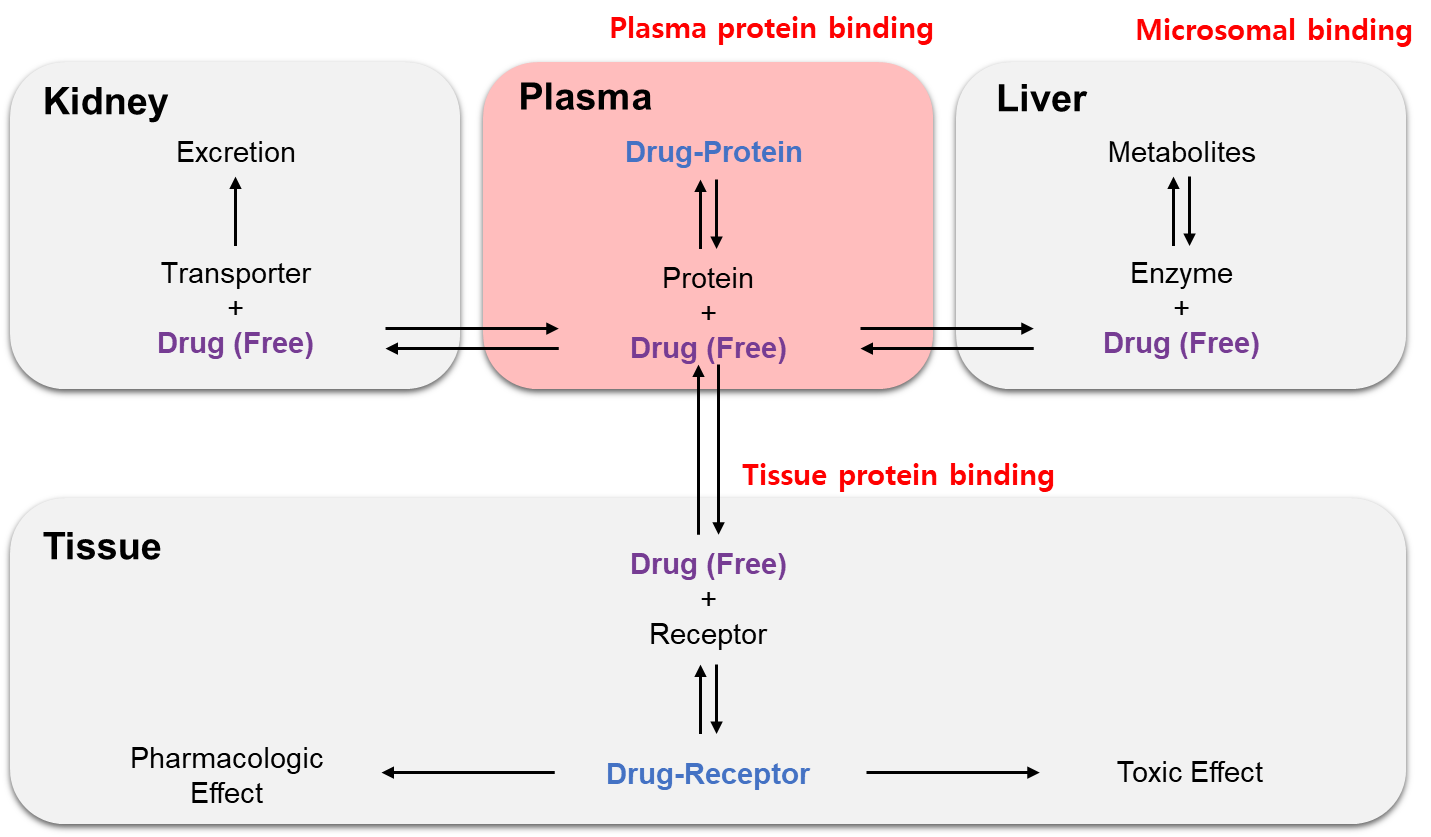
\includegraphics[width=1\linewidth]{media-03/image1} 

}

\caption{자유약물가설의 개략도}\label{fig:03-01}
\end{figure}



약물의 단백결합 평가는 약물동태의 분포와 관련된 평가 중 하나이지만, 그 외 약효의 설명 또는 유효농도 예측, 안전성 평가 및 약물상호작용의 위험도를 평가하는데도 활용된다. 약물의 단백결합은 plasma, tissue 그리고 microsome 등 여러 종류의 단백질에 대하여 평가하지만, 이번 장에서는 혈장에서의 단백결합 평가 방법 및 평가 시 고려해야할 사항에 대해 기술하여 이해를 돕고자 한다.

\hypertarget{uxd608uxc7a5-uxb0b4-uxc8fcuxc694-uxc57duxbb3c-uxacb0uxd569-uxb2e8uxbc31uxc9c8}{%
\section{혈장 내 주요 약물 결합 단백질}\label{uxd608uxc7a5-uxb0b4-uxc8fcuxc694-uxc57duxbb3c-uxacb0uxd569-uxb2e8uxbc31uxc9c8}}

혈장에서 약물이 주로 결합할 수 있는 단백질로는 albumin,
α1-acid-glycoprotein (AGP), lipoprotein 그리고 globulin 등이 있다. 이 중
albumin은 혈장 내 단백질 구성 성분 중 50\% 이상을 차지하고 있어, 혈장 내
단백질 성분 중 가장 많은 양을 차지하고 있다. 또한 albumin은 결합 부위도
8개를 가지고 있으며, 이 중 2개의 결합부위에는 주로 산성이나 중성인
약물들이 결합하게 된다. 다음으로 AGP, lipoprotein 순으로 약물들이 많이
결합하게 되는데, 염기성 약물은 주로 AGP와 결합하고, lipoprotein은 산성,
중성 및 염기성 약물이 일부 결합하며, globulin에는 비타민, 스테로이드가
결합하는 것으로 알려져 있다.

\hypertarget{uxd608uxc7a5-uxb2e8uxbc31uxacb0uxd569-uxd3c9uxac00-uxbc29uxbc95}{%
\section{혈장 단백결합 평가 방법}\label{uxd608uxc7a5-uxb2e8uxbc31uxacb0uxd569-uxd3c9uxac00-uxbc29uxbc95}}

혈장 내 단백질과 약물의 결합을 평가하는 방법으로는 형광분석법
(fluorescence spectroscopy), 크로마토그래피 및 모세관 전기영동법
(Chromatography and capillary electrophoresis),
미세투석법(Microdialysis), 평형투석 (Equilibrium Dialysis), 한외여과
(Ultrafiltration) 그리고 초고속 원심분리 (Ultracentrifugation)과 같이
다양한 방법이 개발되어 있다. 가장 일반적으로 사용되는 평가 방법은
평형투석, 한외여과 및 초고속 원심분리 방법이며, 이 세 가지 방법에 대해서
자세히 기술해 보도록 하겠다.

\hypertarget{uxd3c9uxd615uxd22cuxc11duxbc95-equilibrium-dialysis}{%
\subsection{평형투석법 (Equilibrium Dialysis)}\label{uxd3c9uxd615uxd22cuxc11duxbc95-equilibrium-dialysis}}

평형투석법 (Equilibrium Dialysis)은 여러 단백결합 평가 방법 중 gold
standard로 알려져 있다. 아래의 그림 \ref{fig:03-02}은 평형투석법으로 약물의 혈장
단백결합을 평가할 때 많이 사용되는 RED (Rapid Equilibrium Dialysis)
device를 이용한 시험 방법을 나타낸 것이다. Plasma chamber (Red)에
시험물질을 첨가한 혈장을 넣고, Buffer chamber (White)에는 phosphate
buffer를 넣어준 후 평형상태에 도달할 수 있도록 충분한 시간 (약
4-24시간)동안 37 ℃에서 배양시킨다. 이 과정에서 Plasma chamber 내 약물은
혈장 내 단백질과 결합을 하게 되고, 결합하지 않은 약물만이 반투과성 막을
통과하여 Buffer chamber로 확산 이동을 하게 된다. 그리고 배양이 끝난 후
Plasma 및 Buffer chamber에서의 약물 농도를 측정하여 식 \eqref{eq:eq03-01}과 같이
계산하면, 단백결합율 (fraction bound, f\textsubscript{b}) 및 비결합 분획 (fraction
unbound, f\textsubscript{u})을 산출할 수 있다.

\begin{figure}

{\centering 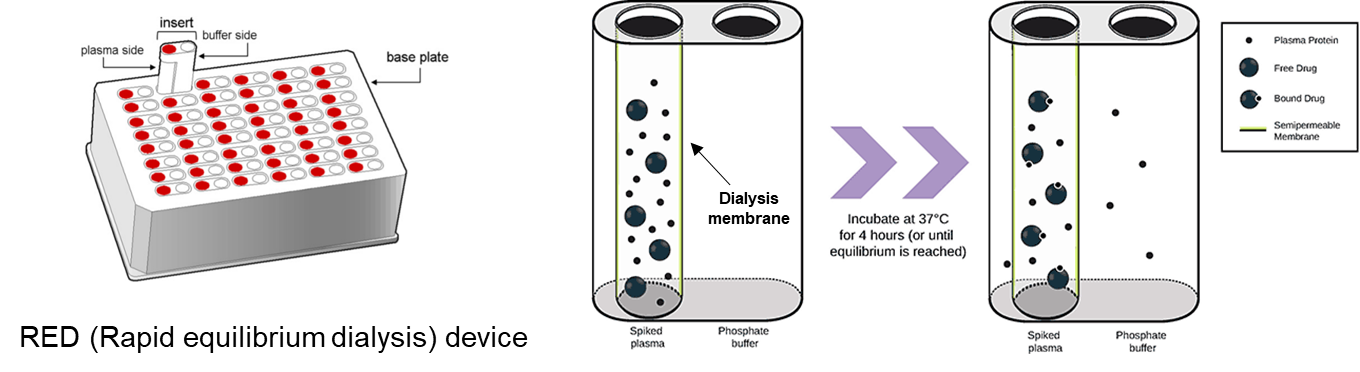
\includegraphics[width=1\linewidth]{media-03/image2} 

}

\caption{평형투석법 (Equilibrium Dialysis)}\label{fig:03-02}
\end{figure}



\begin{equation}
\% Bound = \frac{Conc.\ of\ \mathbf{buffer}\ chamber}{Conc.of\ \mathbf{sample}\ chamber} \times 100\ (\%)
\\ \%\ Unbound = 100 - \%\ Bound
\\ f_u = \ \frac{\%\ Unbound}{100}
\label{eq:eq03-01} 
\end{equation}

반투과성 막을 기준으로 Plasma와 Buffer chamber가 구분되어 있기는 하지만,
결합하지 않은 유리 상태의 약물이 막을 자유롭게 이동할 수 있어
평형상태에서의 단백결합율을 측정할 수 있다는 장점이 있다. 이 점이
평형투석법이 단백결합 평가 시 가장 많이 쓰이며 표준시험법으로 여겨지는
이유다. 반면 4시간 이상, 길게는 24시간 이상 배양을 해야 하므로,
혈장에서의 안정성이 낮은 약물인 경우 낮은 회수율 (recovery)이 나올 수
있으며, Plasma 및 Buffer chamber 간 용매의 이동으로 인해 volume의 변화가
나타날 수 있다.

\hypertarget{uxd55cuxc5ecuxacfc-ultrafiltration-uxd3c9uxac00uxbc95}{%
\subsection{한여과 (ultrafiltration) 평가법}\label{uxd55cuxc5ecuxacfc-ultrafiltration-uxd3c9uxac00uxbc95}}

한여과 (ultrafiltration) 평가법은 결합하지 않은 약물이 반투과성 막을
통과한다는 점이 앞서 설명하였던 평형투석법과 유사하지만, 평형상태에서
Buffer 내 약물 농도를 측정하는 평형투석법과 달리 일정 시간이 지난 후
원심분리를 통해 막을 통과한 여과액 (filtrate)에서의 약물 농도를
측정한다는 차이가 있다. 그림 \ref{fig:03-03}과 같이 평가 장치의 하단부에
반투과성 막이 있으며 막의 위쪽에 약물과 혈장을 함께 넣은 후 원심분리를
하면 유리 상태의 약물만이 막을 통과한 여과액에 모이게 된다. 분자량이 큰
혈장 내 단백질 및 이와 결합한 약물은 막을 투과할 수 없다. 이렇게 얻어진
여과액에서의 약물 농도를 측정하고, 원심분리 전 완충액 내 약물 농도를
측정하여 식 \eqref{eq:eq03-02}에 따라 계산하면, 비특이적 결합 (non-specific binding,
NSB) 및 비결합 분획 (fraction unbound, f\textsubscript{u})을 산출할 수 있다.

\begin{figure}

{\centering 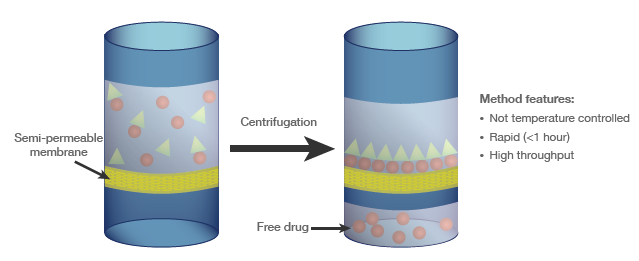
\includegraphics[width=1\linewidth]{media-03/image3} 

}

\caption{한여과 (ultrafiltration) 평가법}\label{fig:03-03}
\end{figure}



\begin{equation}
NSB = \frac{C_{pre} - C_{post}}{C_{pre}} \\
f_u = \frac{F_f}{[(1-NSB) \times F_e]}
\label{eq:eq03-01} 
\end{equation}

C\textsubscript{pre}: initial conc. of compound before filtration in buffer\\
C\textsubscript{post}: recovered conc. of compound after ultrafiltration in buffer\\
Ff: the area ratio of compound after ultrafiltration\\
Fe: the area ratio of compound before ultrafiltration\\
NSB: non-specific binding

한여과 평가법의 장점은 평형투석법과 달리 빠른 시간 내 평가가 가능하므로,
비교적 혈장에서 불안정한 약물도 평가가 가능하다는 것이다. 반면
원심분리에 의해 반투과성 막이 손상되는 경우도 있고, 다른 평가 방법에
비해 비특이적 결합이 높다는 단점이 있다.

\hypertarget{uxcd08uxc6d0uxc2ecuxbd84uxb9ac-ultracentrifugation-uxd3c9uxac00uxbc95}{%
\subsection{초원심분리 (Ultracentrifugation) 평가법}\label{uxcd08uxc6d0uxc2ecuxbd84uxb9ac-ultracentrifugation-uxd3c9uxac00uxbc95}}

초원심분리 (Ultracentrifugation) 평가법은 초원심분리용 tube에 약물과
혈장을 넣고, 장기간 동안 초원심분리 (예: 500,000 g, 10-24 시간) 하여
단백질을 바닥에 침전시킨 후 aqueous layer 내 결합하지 않은 약물의 농도를
측정한다 (그림 \ref{fig:03-04}). 이 방법은 앞서 설명한 평형투석법이나 한여과
평가법과는 달리 비특이적 결합이 없다는 장점이 있으나, 초원심분리 후
생기는 upper layer (지질층)에 약물이 결합할 수 있어 이보다 아래의
aqueous layer를 취하는 과정에서 시료가 오염될 수 있다. 그리고 고가의
장비인 초원심분리기가 있어야만 이 방법으로 평가가 가능하다는 단점이
있으며, 다른 방법과 비교했을 때 상대적으로 단백결합율이 낮게 평가되는
경향이 있다.

\begin{figure}

{\centering 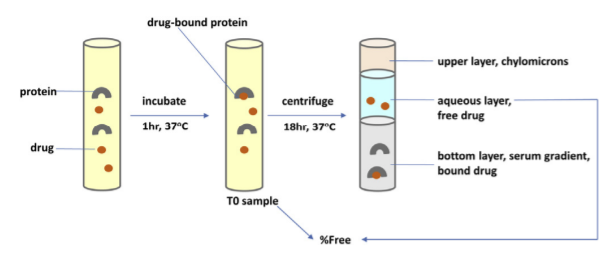
\includegraphics[width=1\linewidth]{media-03/image4} 

}

\caption{초원심분리 (Ultracentrifugation) 평가법}\label{fig:03-04}
\end{figure}



\hypertarget{uxd608uxc7a5uxb2e8uxbc31uxacb0uxd569-uxacb0uxacfc-uxd574uxc11d-uxbc0f-uxd65cuxc6a9}{%
\section{혈장단백결합 결과 해석 및 활용}\label{uxd608uxc7a5uxb2e8uxbc31uxacb0uxd569-uxacb0uxacfc-uxd574uxc11d-uxbc0f-uxd65cuxc6a9}}

혈장단백결합 결과의 해석은 궁극적으로 혈장단백결합율의 높고 낮음을
분류하는 것이다. 혈장단백결합율의 높고 낮음을 나누는 정형화된 기준은
없으며, 시험 기관 혹은 문헌 마다 그 기준이 상이하다. 일반적으로
혈장단백결합율이 90\% 이상이면 높은 것으로 분류하지만, 최근 highly
potent한 약물을 개발하는 경우가 많아지면서 이에 따라 lipophilicity가
증가되어, 많은 약물들이 90\% 이상의 높은 혈장단백결합율을 보이고 있다.
이러한 추세를 반영하면, 혈장단백결합율이 98\%이상이면 high, 90-98\%를
moderate 그리고 90\% 이하이면 low로 분류하는 것이 보다 현실적인 기준일
것으로 판단된다.

약효 측면에서는 자유약물가설에 따라 혈장단백율이 낮을수록 유리한 약물로
생각할 수 있다. 그러나 유리 상태의 약물은 빠르게 대사 및 배설될 수 있고,
혈장 내 유리 상태의 약물 비율이 낮아지면 결합된 약물이 분리되어 다시
평형을 이루게 되므로 혈장단백결합율의 좋고 나쁨을 판단하기는 어렵다.
약물상호작용 측면에서 보면, 높은 단백결합율을 보이는 약물의 경우
약물상호작용의 위험이 높다고 판단할 수 있다. 예를 들어 단백결합율이
99.9\% (fraction bound, f\textsubscript{b} = 0.999)인 약물이 병용투여한 약물에 의해
단백결합율이 99.8\%로 감소된다면, 단백결합율은 0.1\%의 차이로 서로 유사한
것처럼 보이나, 이 때 비결합분획 (fraction unbound, f\textsubscript{u})는 0.01에서
0.02로 2배가 증가된 것이므로 이는 매우 큰 차이라 할 수 있다. 안전역
(Therapeutic index)이 낮은 약물인 경우 위와 같은 약물상호작용에 따른
단백결합율의 변화가 부작용과 연관될 수 있어 주의가 필요하다.

혈장단백결합율은 약효, 독성, 약물상호작용의 위험도를 설명하거나
예측하는데 활용된다. 예를 들면, 자유약물가설에 따라 약물의 혈중 농도에
비결합분획을 곱한 혈중 유리 상태의 약물 농도 (free drug concentration)의
time profile과 \emph{in vitro} 시험에서 구한 IC\textsubscript{50} 혹은 EC\textsubscript{50}를 비교하여
약효를 설명하거나 약효 시험의 용량을 결정하기도 하고, \emph{in vitro} hERG
assay에서 구한 IC\textsubscript{50}와 비교하여 약물의 심장 독성에 대한 위험도를
평가하기도 한다. 또한 FDA의 약물상호작용 가이던스에 따라 약물상호작용의
위험도를 평가할 때 산출하게 되는 다양한 R value를 구하기 위해서도
혈장단백결합율이 필요하다. 그리고 human PK prediction 과정 중
클리어런스나 생체이용률을 예측하기 위한 IVIVE (In Vitro-In Vivo
Extrapolation)에도 혈장단백결합율이 활용된다.

\hypertarget{uxd608uxc7a5uxb2e8uxbc31uxacb0uxd569-uxd3c9uxac00-uxc2dc-uxace0uxb824uxc0acuxd56d}{%
\section{혈장단백결합 평가 시 고려사항}\label{uxd608uxc7a5uxb2e8uxbc31uxacb0uxd569-uxd3c9uxac00-uxc2dc-uxace0uxb824uxc0acuxd56d}}

\hypertarget{uxb0aeuxc740-uxd68cuxc218uxc728-low-recovery}{%
\subsection{낮은 회수율 (Low recovery)}\label{uxb0aeuxc740-uxd68cuxc218uxc728-low-recovery}}

혈장단백결합을 평가하다 보면, 낮은 회수율 문제가 빈번하게 발생된다. 이
때 낮은 회수율이 나타나는 이유로는 약물의 용해도가 낮거나 혈장 내
안정성이 떨어지는 약물인 경우가 있고, 시험 장치의 plastic ware 또는
반투과성 막에 약물이 결합하는 비특이적 결합 (non-specific binding,
NSB)이 있다. 회수율은 해당 시험계에서의 평가 결과에 대한 신뢰성을
판단하는 기준이기 때문에 만약 회수율이 낮게 나왔다면 재시험을 고려하는
경우가 많다.

만약 평형투석법 평가 시 낮은 회수율의 원인이 약물의 낮은 용해도라면 평가
농도를 낮추어 재시험을 수행할 수 있고, 약물의 혈장 내 안정성이 낮았기
때문이라면 평형투석법이 아닌 한여과법 등의 다른 방법으로 평가하는 것을
고려할 수 있다. 다만 문헌에 따르면, 평형투석법의 경우 회수율이
비결합분획 값에 미치는 영향은 없는 것으로 나타났다 (그림 \ref{fig:fig2table}). 따라서
적어도 전임상 개발 단계가 아닌 lead optimization 단계의 과제라면,
평형투석법 평가 시 낮은 회수율로 재시험을 수행하거나, 이를 해결하기 위해
많은 시간적, 물적 및 인적 자원을 사용하는 것은 바람직하지 않다고
보여진다.

\begin{figure}

{\centering 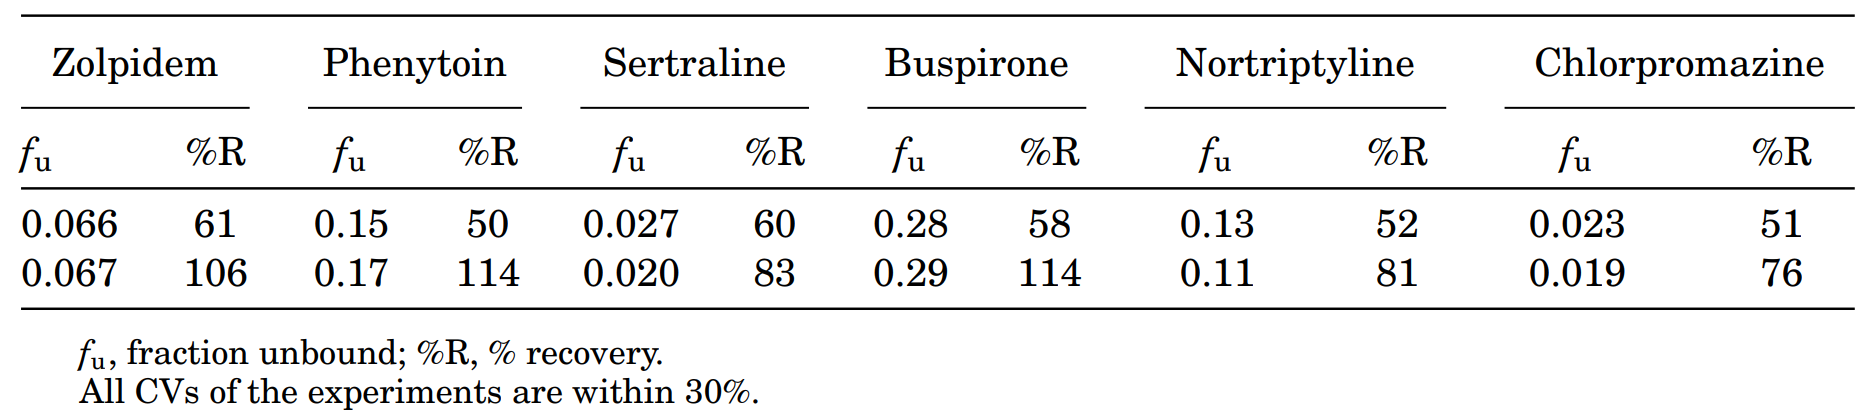
\includegraphics[width=1\linewidth]{media-03/image5} 

}

\caption{회수율이 비결합분획에 미치는 영향}\label{fig:fig2table}
\end{figure}



\hypertarget{uxb192uxc740-uxd608uxc7a5uxb2e8uxbc31uxacb0uxd569uxc744-uxac00uxc9c4-uxc57duxbb3cuxc758-uxd608uxc7a5uxb2e8uxbc31uxacb0uxd569-uxd3c9uxac00uxbc29uxbc95}{%
\subsection{높은 혈장단백결합을 가진 약물의 혈장단백결합 평가방법}\label{uxb192uxc740-uxd608uxc7a5uxb2e8uxbc31uxacb0uxd569uxc744-uxac00uxc9c4-uxc57duxbb3cuxc758-uxd608uxc7a5uxb2e8uxbc31uxacb0uxd569-uxd3c9uxac00uxbc29uxbc95}}

가장 많이 처방되고 있는 100개 약물들의 혈장단백결합율은 98\%이고 (Smith,
Dennis A, 2010), FDA에서 승인된 189개의 약물들 중 많은 약물들의
혈장단백결합율이 99\% 이상인 것과 같이 최근 매우 높은 혈장단백결합율을
가진 약물들이 많이 개발되고 있는 추세이다 (그림 \ref{fig:03-05}).

\begin{figure}

{\centering 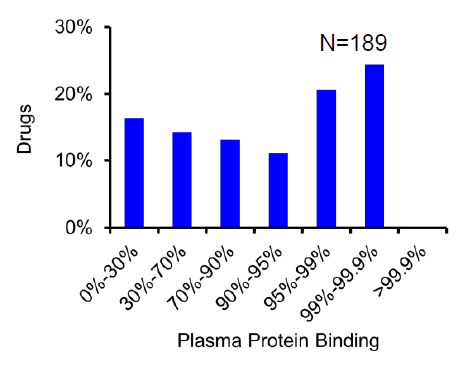
\includegraphics[width=1\linewidth]{media-03/image6} 

}

\caption{US FDA에서 승인된 189개 약물의 혈장단백결합율 (\protect\hyperlink{ref-liu2014rational}{Liu, Wright, and Hop 2014})}\label{fig:03-05}
\end{figure}



이 같은 약물을 평형투석법으로 평가 시 Buffer chamber로 이행되는 약물의
양이 너무 적어, Buffer chamber 내 약물 농도를 분석할 때 정량한계의
문제로 인해 단백결합율을 구하지 못하는 경우가 있다. 이럴 때는 혈장을
희석하여 단백결합율을 평가하는 방법을 고려해볼 수 있다. 주의할 점은 기존
평형투석법과 동일하게 RED device를 이용해 평가를 수행하되, 희석한 혈장을
첨가하여 평가를 진행하므로 비결합분획을 계산할 때 반드시 희석배수를
보정하여 산출해야 한다는 것이다. 아래의 식 \eqref{eq:eq03-03}은 혈장을 10배 희석하여
사용했을 때 비결합분획을 계산하는 수식을 나타낸 예시이다.

\begin{equation}
\% Bound = \frac{Conc.of\ \mathbf{buffer}\ chamber}{Conc.of\ \mathbf{sample}\ chamber} \times 100(\%) \\
\% Unbound = 100 - \% Bound \\
f_{u\ 10\%} = \ \frac{\%_{unbound}}{100} \\ 
f_{u\ 100\%} = \ \frac{{\ \ \ f}_{u\ 10\%}}{10\  - 9*f_{u\ 10\%}}
\label{eq:eq03-03} 
\end{equation}

최근에는 이처럼 매우 높은 혈장단백결합율을 보이는 화합물의 비결합분획을 산출할 수 있도록 고안된 제품 (TRANSIL High Sensitivity Binding Kit\footnote{\url{https://sovicell.com/products/tpb-0400-0135}}) 도 있어, 높은 단백결합율로 인해 어려움을 겪을 때 이러한 장치를 활용하는 것도 추천한다.

\hypertarget{uxb9fauxc74cuxb9d0-2}{%
\section{맺음말}\label{uxb9fauxc74cuxb9d0-2}}

이상으로 ADME의 기초자료: Physicochemical properties에서 혈장단백결합 평가 방법 및 평가 시 고려사항에 대해 알아보았다. 혈장단백결합 평가는 분포에 관련된 평가 중 하나이며 단백결합율의 높고 낮음이 약물의 우수성을 나타내지는 않는다. 하지만 혈장단백결합율은 약효, 독성, 약물상호작용, 임상 PK 예측 등 신약개발의 다양한 영역에서 결과의 해석, 용량결정 및 예측에 활용된다. 따라서, 혈장단백결합을 이해하고 적절한 방법으로 평가하는 것이 필요하겠다.

\textbf{참고문헌}

(편집자: 이 참고문헌은 모두 인용 위치가 본문 내에서 구체적으로 표시되어야 합니다.)

\begin{enumerate}
\def\labelenumi{\arabic{enumi}.}
\tightlist
\item
  Tonika; Gan, Liang-Shang.~Plasma protein binding: From discovery to development. Journal of Pharmaceutical Sciences, 102(9), 2953--2994, 2013.
\item
  Van Liempd, Sebastiaan; Morrison, Denise; Sysmans, Leen; Nelis, Paul; Mortishire-Smith, Russell. Development and Validation of a Higher-Throughput Equilibrium Dialysis Assay for Plasma Protein Binding. Journal of Laboratory Automation, 16(1), 56--67, 2011.
\item
  Li Di; John P. Umland; Patrick E. Trapa; Tristan S. Maurer. Impact of recovery on fraction unbound using equilibrium dialysis. 101(3), 1327--1335, 2012.
\item
  Liu, Xingrong; Wright, Matthew; Hop, Cornelis E. C. A. Rational Use of Plasma Protein and Tissue Binding Data in Drug Design. Journal of Medicinal Chemistry, 57(20), 8238--8248, 2014.
\item
  Buscher, Brigitte; Laakso, Sirpa; Mascher, Hermann; Pusecker, Klaus; Doig, Mira; Dillen, Lieve; Wagner-Redeker, Winfried; Pfeifer, Thomas; Delrat, Pascal; Timmerman, Philip. Bioanalysis for plasma protein binding studies in drug discovery and drug development: views and recommendations of the European Bioanalysis Forum. Bioanalysis, 6(5), 673--682, 2014.
\item
  Edward H. Kerns and Li Di, Drug-like properties: Concepts, Structure Design and Methods.
\item
  Everything you need to know about ADME, 3rd Edition, Cyprotex
\end{enumerate}

\hypertarget{part-uxb300uxc0ac-uxbc0f-uxc218uxc6a9uxccb4}{%
\part{대사 및 수용체}\label{part-uxb300uxc0ac-uxbc0f-uxc218uxc6a9uxccb4}}

\hypertarget{uxb300uxc0ac-uxae30uxc9c8uxb85cuxc758-uxd6c4uxbcf4-uxbb3cuxc9c8-uxd2b9uxc131-uxd3c9uxac00}{%
\chapter{대사 기질로의 후보 물질 특성 평가}\label{uxb300uxc0ac-uxae30uxc9c8uxb85cuxc758-uxd6c4uxbcf4-uxbb3cuxc9c8-uxd2b9uxc131-uxd3c9uxac00}}

\Large\hfill

배수현
\normalsize

\hypertarget{uxc11cuxb860-3}{%
\section{서론}\label{uxc11cuxb860-3}}

대사 과정은 체내에서 약물을 체외로 배출하는 주요한 과정 중 하나이다. 체내에 흡수되어 혈액을 따라 전신 순환하는 약물은 조직으로 이행되며, 간에서 대사(metabolism)되어 담즙이나 소변으로 배설되거나, 대사과정을 거치지 않고 곧바로 배설(excretion)되기도 한다. 대사는 약물의 제거뿐만 아니라, 흡수에도 중요한 역할을 한다. 경구로 약물을 복용하게 되면, 약은 위장관과 간을 통과한 후, 전신으로 흡수되어 조직으로 약물이 이행된다. 이 과정에서 위장관과 간에 존재하는 대사효소에 의해 제거되고 살아남은 약물만 전신으로 흡수될 수 있다. 이를 초회 통과효과(first-pass effect)라고 한다. 약동학에서 약물의 제거(elimination)과정은 대사와 배설을 포함하며, 이 단원에서는 대사 과정에 관하여 자세히 다룰 예정이다.

\hypertarget{uxb300uxc0ac-uxacfcuxc815}{%
\section{대사 과정}\label{uxb300uxc0ac-uxacfcuxc815}}

대사 과정은 체내에서 약물이 제거되는데 필수적인 과정이며, 대사 효소에 의하여 약물이 대사체 형태로 변환(biotransformation)되는 일련의 과정을 일컫는다. 약은 이물질(xenobiotics)이며, 대부분의 약물은 친유성(lipophilic)을 띄고 있어 혈장단백과의 결합률이 높은 편인데, 대사 과정을 통해 약물은 친수성(hydrophilic)이 증가하게 되며, 신장으로의 배설이 용이하게 된다. 대사 과정을 통해 대부분의 약은 약리활성 및 독성을 잃게 되나, 때때로 생성된 대사체가 약효 및 부작용을 나타내는 경우가 있다. 이를 reactive metabolite (또는 reactive intermediate)이라고 하며, 주로 생체 내 고분자인 단백질이나 핵산과 공유 결합하여 세포독성, 유전독성 등을 일으킨다. 잘 알려진 예로 아세트아미노펜의 대사과정을 살펴보자(그림 \ref{fig:04-01}). 아세트아미노펜은 대부분 간에서 phase II 대사를 통해 독성 및 활성이 없는 대사체를 생성하여 체외로 배출되는데, 아세트아미노펜을 과량 복용하게 되면, phase I 대사를 거쳐 높은 반응성을 지닌 reactive metabolite인 \emph{N}-acetyl-\emph{p}-benzoquinone imine (NAPQI)를 생성하게 된다. 생성된 NAPQI가 phase II 대사를 거쳐 글루타치온 포합체를 생성하지 못하면, 간세포 내의 단백질 및 핵산과 결합하여 궁극적으로 세포를 파괴하여 간 독성을 나타낸다.

\begin{figure}

{\centering 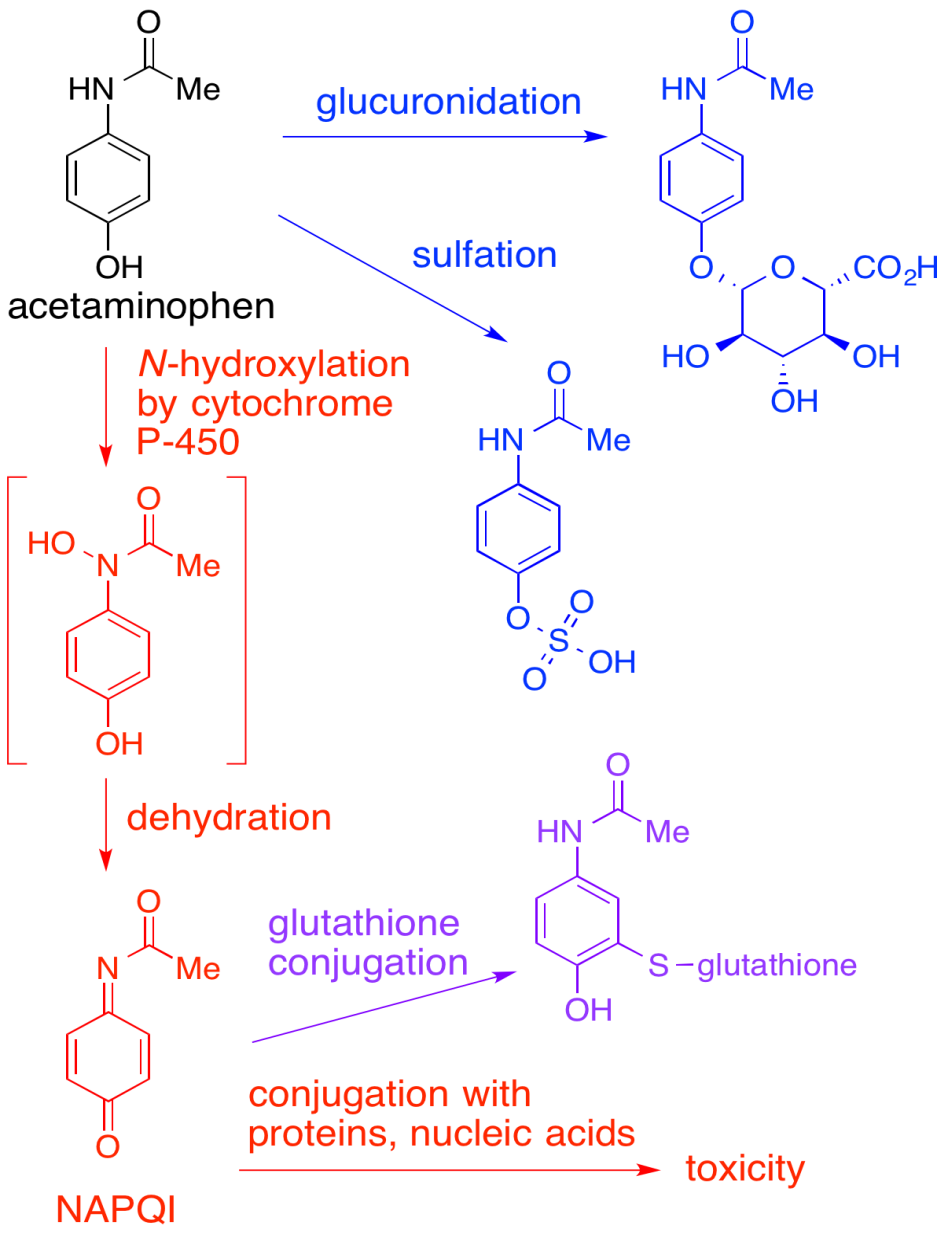
\includegraphics[width=1\linewidth]{media-04/image1} 

}

\caption{아세트아미노펜의 대사과정. (위키피디아 NAPQI 검색 후, 발췌)}\label{fig:04-01}
\end{figure}



대사 과정에는 phase I 대사와 phase II 대사가 있으며, 각각의 과정에 관여하는 대사 효소의 종류와 생성되는 대사체의 성질도 다르다. 일반적으로 phase I 대사를 통해 약물은 산화, 환원, 또는 가수분해 등의 반응을 거치게 되고, 이로 인해 배설 및 다음 대사과정에 용이한 작용기를 가지게 되고, 반응성이 증가하게 된다. 그리고 phase II 대사를 통해 glucuronide, sulfate 등의 포합체가 생성되어 수용성이 증가하게 되며, 신장이나 담즙을 통해 배설되게 된다. 일반적으로 phase I → phase II 대사를 순차적으로 거쳐 약물이 체외로 배설된다고 알려져 있으나, 약물의 구조와 작용기의 유무에 따라 phase I 대사 또는 phase II 대사 각각 거치거나, phase II 대사 이후 phase I 대사과정을 거치는 등 다양한 방법으로 변환되어 체외 배설된다. 다음 장에서 대사 효소에 대하여 자세히 알아보자.

\hypertarget{uxb300uxc0ac-uxd6a8uxc18c}{%
\section{대사 효소}\label{uxb300uxc0ac-uxd6a8uxc18c}}

앞서 말했듯이, 대사 과정은 크게 phase I 대사 및 phase II 대사로 나뉜다.

\hypertarget{phase-i-uxb300uxc0ac}{%
\subsection{Phase I 대사}\label{phase-i-uxb300uxc0ac}}

Phase I 대사는 약물을 산화, 환원, 또는 가수분해 시켜 약물의 반응성을
증가시키는 과정이다. Phase I 대사의 가장 중요한 대사 효소는 cytochrome
P450 (CYP)이며, 약물의 산화반응에 관여한다. CYP는 헴(heme) 단백질로 간의
소포체(endoplasmic reticulum, ER)에 주로 존재하며, NADPH와 O\textsubscript{2}를 이용한
산화 환원 반응을 통해 약물을 대사체로 변환(주로 산화)시킨다. CYP3A4/5는
간에 많이 분포하고 있지만, 위장관에도 분포하고 있어, CYP3A4/5로 대사되는
약물의 위장관 및 간 초회 통과 효과에 영향을 미친다.

CYP는 다음과 같이 명명된다(그림 \ref{fig:04-02}). 염기서열이 40\% 이상
상동(homology)하면 숫자를 이용하여 같은 'family'로 분류하며, 그 중에서도
55\% 이상 상동이면 'subfamily'가 같으며, 이는 알파벳 대문자로 표시한다.
그리고 'specific isoform'을 숫자로 표시하여 동일한 CYP 효소 (동효소,
isozyme)임을 명명한다. 그리고 'allele number'를 통해 CYP 동효소의
유전형을 표기한다. 야생형(wild type)의 경우, 주로 *1으로 표기되며,
아미노산 변이 및 돌연변이에 의해 유전형은 *2, *3, *13등과 같이
표기된다.

약물 대사에 관여하는 주요한 CYP 동효소는 CYP1A2, CYP2B6, CYP2C8, CYP2C9,
CYP2C19, CYP2D6, CYP3A4/5이며, 신약개발 시 미국 Food and Drug
Administration (FDA) 및 European Medicines Agency (EMA)에서는 위의
동효소에 대한 대사능 및 저해(유도)능을 확인하도록 가이던스에 권고하고
있다 (\protect\hyperlink{ref-studies2020cytochrome}{Studies 2020}; \protect\hyperlink{ref-european2012guideline}{Agency 2012}).

\begin{figure}

{\centering 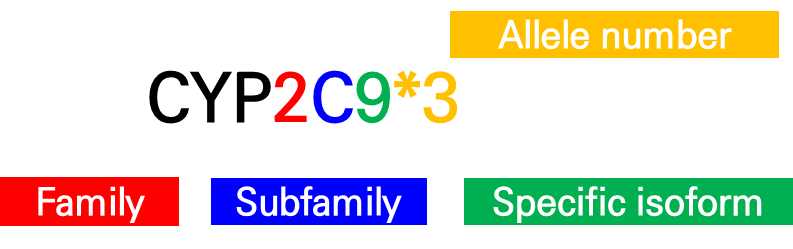
\includegraphics[width=1\linewidth]{media-04/image2} 

}

\caption{CYP 동효소의 명명법}\label{fig:04-02}
\end{figure}



Phase I 대사 효소 중 하나인 flavin-containing monooxygenase (FMO)에
의해서도 약물이 대사된다. FMO를 매개하는 약물상호작용의 경우는 흔지
않으며, 주로 유전형에 따른 FMO의 발현 정도가 약물의 대사에 영향을
미친다. FMO 동효소 중에서 FMO3는 간에 주로 분포하며, 유전적 다형성을
지니며, amphetamine, tamoxifen, clozapine, phenothiothiazine 계열 약물의
대사에 관여한다. FMO1은 주로 신장에 분포하여 신장으로 배설되는 약물의
대사에 중요한 역할을 하는 것으로 알려져 있다.

Phase I 대사 중 산화 과정에 대하여 알아보자. 주로 CYP 동효소에 의해
oxidation, dealkylation, hydroxylation 등이 일어나며, CYP 외의 FMO와
monoamine oxidase (MAO) 등에 의한 산화 과정도 이에 포함된다. 이 과정들에
대한 예는 표 \ref{tab:table04-01}에 자세히 나와 있다.

\begin{longtable}[]{@{}
  >{\raggedright\arraybackslash}p{(\columnwidth - 4\tabcolsep) * \real{0.3333}}
  >{\raggedright\arraybackslash}p{(\columnwidth - 4\tabcolsep) * \real{0.3333}}
  >{\raggedright\arraybackslash}p{(\columnwidth - 4\tabcolsep) * \real{0.3333}}@{}}
\caption{\label{tab:table04-01} 약물의 대사 과정 - 산화 과정}\tabularnewline
\toprule()
\begin{minipage}[b]{\linewidth}\raggedright
Reaction
\end{minipage} & \begin{minipage}[b]{\linewidth}\raggedright
Structural formula
\end{minipage} & \begin{minipage}[b]{\linewidth}\raggedright
Drugs
\end{minipage} \\
\midrule()
\endfirsthead
\toprule()
\begin{minipage}[b]{\linewidth}\raggedright
Reaction
\end{minipage} & \begin{minipage}[b]{\linewidth}\raggedright
Structural formula
\end{minipage} & \begin{minipage}[b]{\linewidth}\raggedright
Drugs
\end{minipage} \\
\midrule()
\endhead
I. CYP-dependent oxidations & & \\
Aliphatic hydroxylation & 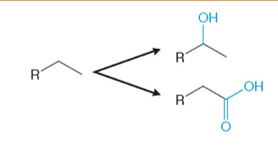
\includegraphics{./media-04/image3.png} & Barbiturates, cyclosporine, ibuprofen \\
& 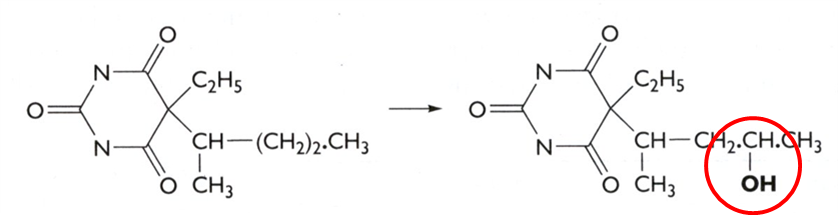
\includegraphics{./media-04/image4.png} & \\
Aromatic hydroxylation & 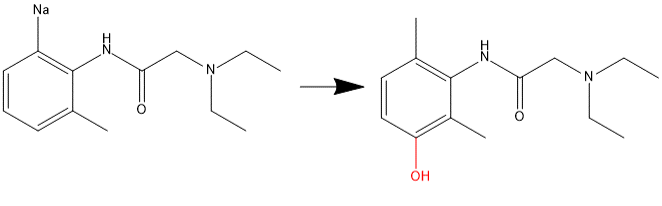
\includegraphics{./media-04/image5.png} & Phenytoin, propranolol \\
N-dealkylation & 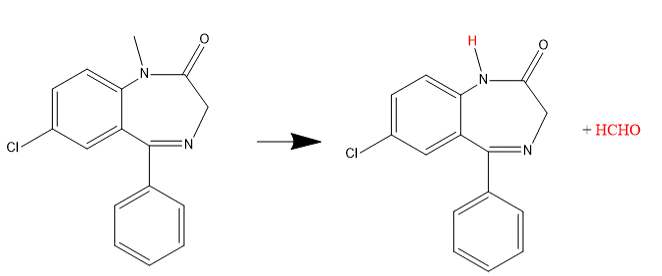
\includegraphics{./media-04/image6.png} & Sildenafil, diazepam \\
O-dealkylation & 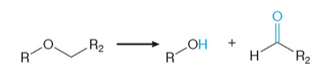
\includegraphics{./media-04/image7.png} & Codeine \\
S-oxidation & 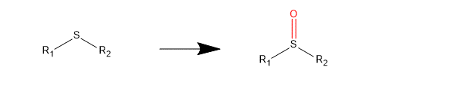
\includegraphics{./media-04/image8.png} & Cimetidine, phenothiazine \\
N-oxidation & 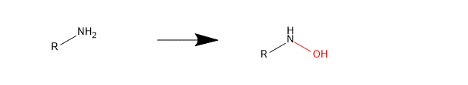
\includegraphics{./media-04/image9.png} & Quinidine \\
Desulfuration & 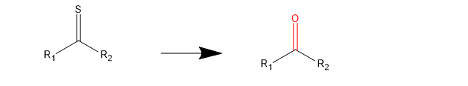
\includegraphics{./media-04/image10.png} & Thiopental \\
Epoxidation & 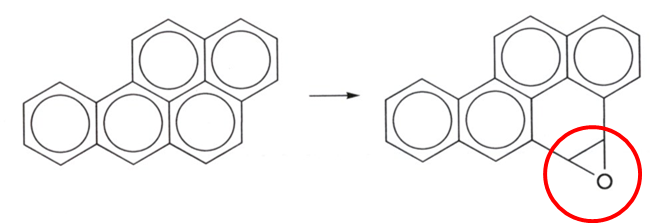
\includegraphics{./media-04/image11.png} & Carbamazepine \\
II. CYP-independent oxidations & & \\
Alcohol dehydrogenation, Aldehyde dehydrogenation & 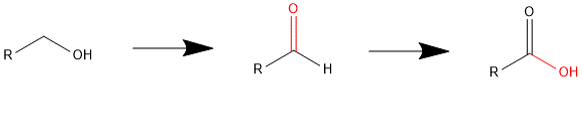
\includegraphics{./media-04/cap01.png} & Ethanol, pyridoxine \\
Oxidative deamination & 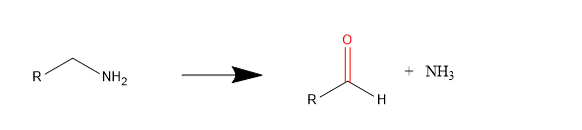
\includegraphics{./media-04/cap02.png} & Histamine, norepinephrine \\
Decarboxylation & 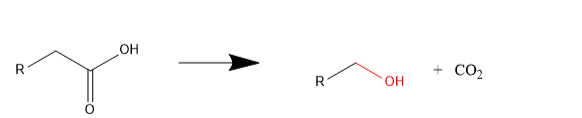
\includegraphics{./media-04/cap03.png} & Levodopa \\
\bottomrule()
\end{longtable}

약물의 구조에 따라 산화 과정 뿐만 아니라, 환원 및 가수분해 과정을
통해서도 약물이 대사된다(표 \ref{tab:table04-02}). 환원에 의한 대사과정은 산화 및 가수분해 보다 흔치 않다.
가수분해는 주로 간에 존재하는 esterase (ES)에 의해 ester hydrolysis 되며, 약물의 구조 상 amide hydrolysis, epoxide hydrolysis 될 수 있다.

\begin{longtable}[]{@{}
  >{\raggedright\arraybackslash}p{(\columnwidth - 4\tabcolsep) * \real{0.3333}}
  >{\raggedright\arraybackslash}p{(\columnwidth - 4\tabcolsep) * \real{0.3333}}
  >{\raggedright\arraybackslash}p{(\columnwidth - 4\tabcolsep) * \real{0.3333}}@{}}
\caption{\label{tab:table04-02} 약물의 대사 과정 - 환원, 가수분해 과정}\tabularnewline
\toprule()
\begin{minipage}[b]{\linewidth}\raggedright
Reaction
\end{minipage} & \begin{minipage}[b]{\linewidth}\raggedright
Structural formula
\end{minipage} & \begin{minipage}[b]{\linewidth}\raggedright
Drugs
\end{minipage} \\
\midrule()
\endfirsthead
\toprule()
\begin{minipage}[b]{\linewidth}\raggedright
Reaction
\end{minipage} & \begin{minipage}[b]{\linewidth}\raggedright
Structural formula
\end{minipage} & \begin{minipage}[b]{\linewidth}\raggedright
Drugs
\end{minipage} \\
\midrule()
\endhead
I. Reduction & 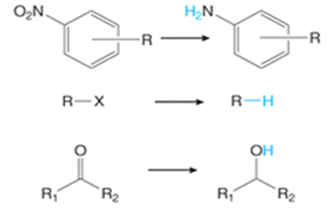
\includegraphics{./media-04/cap04.png} & Chloramphenicol, methadone, naloxone \\
II. Hydrolysis & 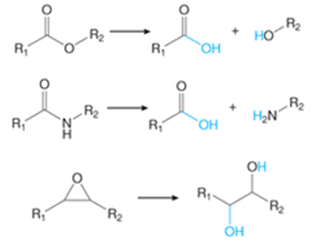
\includegraphics{./media-04/cap05.png} & Aspirin, procaine, lidocaine, indomethacin, irinotecan \\
\bottomrule()
\end{longtable}

\hypertarget{phase-ii-uxb300uxc0ac}{%
\subsection{Phase II 대사}\label{phase-ii-uxb300uxc0ac}}

Phase II 대사는 모약물 및 대사체의 작용기에 glucuronide, sulfate,
acetate, glutathione 등의 포합체를 붙여 약물의 수용성을 증가시킨다. 이
과정을 통해 약물은 소변이나 담즙을 통해 체외로 배설된다. 대표적인 대사
효소로는 uridine 5\textquotesingle-diphospho-glucuronosyltransferases
(UDP-glucuronosyltransferases, UGTs), sulfotransferases (SULTs),
\emph{N}-acetyltransferases (NATs), glutathione S-transferase (GST) 등이
있다.

글루크론산화(glucuronidation)은 UGT 동효소에 의해 일어나며, UGT는 UGT1과
UGT2의 2개의 family로 분류된다. 기질로는 bilirubin, irinotecan의
활성대사체인 SN-38 (이하 UGT1A1), morphine, efavirenz (이하 UGT2B7) 등이
대표적이다. 글루크론산화된 대사체는 소변 또는 담즙으로 배설되는데,
담즙으로 배설된 대사체는 소장에 존재하는 β-glucuronidase에 의해 포합체가
떨어져나가 모약물 형태로 다시 위장관을 통해 재흡수 될 수 있다.

황산화(sulfation) 및 아세틸화(acetylation)은 각각 SULT와 NAT에 의해
일어나며, acetaminophen과 isoniazid가 각각 SULT와 NAT의 기질로 알려져
있다.

각 대사 과정들에 대한 예는 표 \ref{tab:table04-03}에 자세히 나와 있다.

\begin{longtable}[]{@{}
  >{\raggedright\arraybackslash}p{(\columnwidth - 4\tabcolsep) * \real{0.1935}}
  >{\raggedright\arraybackslash}p{(\columnwidth - 4\tabcolsep) * \real{0.6022}}
  >{\raggedright\arraybackslash}p{(\columnwidth - 4\tabcolsep) * \real{0.1828}}@{}}
\caption{\label{tab:table04-03} 약물의 대사 과정 - Phase II}\tabularnewline
\toprule()
\begin{minipage}[b]{\linewidth}\raggedright
Reaction
\end{minipage} & \begin{minipage}[b]{\linewidth}\raggedright
Structural formula
\end{minipage} & \begin{minipage}[b]{\linewidth}\raggedright
Drugs
\end{minipage} \\
\midrule()
\endfirsthead
\toprule()
\begin{minipage}[b]{\linewidth}\raggedright
Reaction
\end{minipage} & \begin{minipage}[b]{\linewidth}\raggedright
Structural formula
\end{minipage} & \begin{minipage}[b]{\linewidth}\raggedright
Drugs
\end{minipage} \\
\midrule()
\endhead
I.
Glucuronidation & 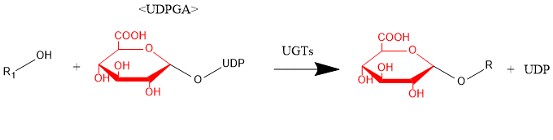
\includegraphics[width=3.60417in,height=0.86458in]{./media-04/image15.png} & Diazepam,
digoxin,
acetaminophen,
SN-38, efavirenz \\
& 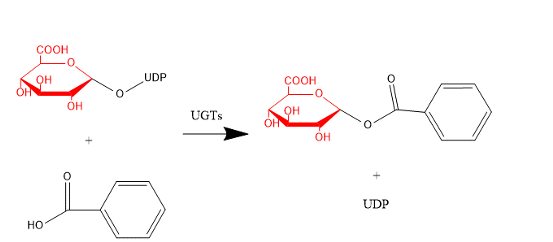
\includegraphics[width=2.94143in,height=1.81684in]{./media-04/image16.png} & \\
II. Acetylation & 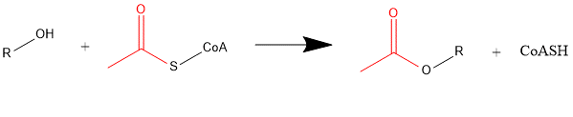
\includegraphics[width=3.13542in,height=0.54167in]{./media-04/image17.png} & Isoniazid,
sulfonamide \\
& 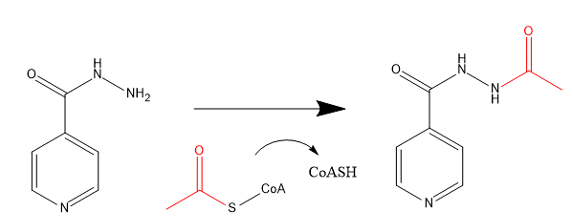
\includegraphics[width=3.20993in,height=1.14513in]{./media-04/image18.png} & \\
III. Sulfation & 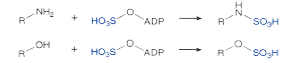
\includegraphics[width=3.125in,height=0.65625in]{./media-04/image19.png} & Methyldopa \\
IV. Glutathione
conjugation & 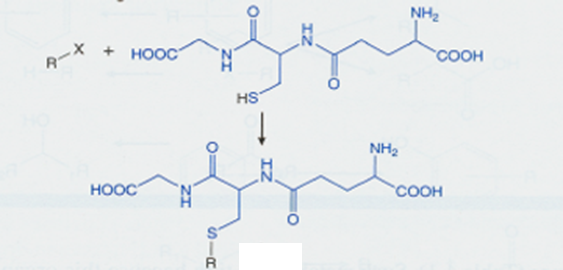
\includegraphics[width=2.71574in,height=1.30235in]{./media-04/image20.png} & Acetaminophen,
valproic acid,
busulfan \\
\bottomrule()
\end{longtable}

\hypertarget{uxb300uxc0ac-uxd2b9uxc131-uxd3c9uxac00}{%
\section{대사 특성 평가}\label{uxb300uxc0ac-uxd2b9uxc131-uxd3c9uxac00}}

약물 대사는 주로 간에서 일어나며, 다양한 \emph{in vitro} 실험을 통해 약물이
어떤 대사효소를 통해 얼마나 대사되는지 확인할 수 있다. 이 단원에서는 \emph{in
vitro} 실험에 사용되는 다양한 시험계의 종류와 그 특성, 대사 특성을
평가하는 시험법, 시험에서 얻을 수 있는 파라미터와 각 파라미터가 의미하는
바에 대하여 순차적으로 알아보자.

\hypertarget{in-vitro-systems}{%
\subsection{In vitro systems}\label{in-vitro-systems}}

약물의 대사를 확인하는 시험계는 세포계(intact cell system),
준세포분획(subcellular fractions), 재조합 효소(recombinant enzyme)
등으로 나눌 수 있다.

\hypertarget{intact-cell-systems}{%
\subsubsection{Intact cell systems}\label{intact-cell-systems}}

대사를 확인하는 세포계는 주로 간세포((cryopreserved) primary
hepatocytes)를 일컫는다. 간세포 자체는 계대 배양이 불가능하여 시험
비용이 비싸며, 사람마다 발현되어 있는 대사효소 및 수송체의
양(abundance)이나 활성(activity)이 상이하기 때문에, 지속적으로 동일한
공여자(donor)의 간세포를 안정적으로 얻을 수 없는 제한점이 있다. 이러한
이유로 간세포 외의 다양한 세포주를 활용하는 대체 실험법이 제안되고
있으며, 효능 평가 및 독성 평가에는 사람 간암 세포주인 HepG2, HepaRG 등을
사용하기도 한다. 하지만, 대사 특성을 평가하는 시험의 경우에는 대사효소
및 수송체 발현 정도가 간암 세포주와 간세포와 다르기 때문에, 대사 특성
평가에 사용되기에는 현재까지 적절하지 않다.

간세포에는 phase I 대사효소 뿐만 아니라, phase II 대사효소가 전부
존재하기 때문에, 종합적인 대사능(intrinsic clearance, CL\textsubscript{int})\textsuperscript{*}을
관찰할 수 있다. 또한, 간세포 내로 약물이 수동확산 또는
수송체(transporter)를 통해 간으로 능동수송(active transport)되어
들어가는 속도(CL\textsubscript{int,pd}, CL\textsubscript{int,uptake})를 측정할 수 있다. 세포
투과성(permeability)이 낮은 약물의 경우, uptake transporter에 의해
간세포 내로 능동수송 된 후 대사되므로, 이러한 수송체의 기질성 여부가
약물의 간대사에 영향을 미칠 수 있다. 간세포 배양방법 (예.
Sandwich-cultured hepatocytes)에 따라 약물의 담즙 배설도
확인(CL\textsubscript{int,bile}) 할 수 있다.

\hypertarget{subcellular-fraction}{%
\subsubsection{Subcellular fraction}\label{subcellular-fraction}}

준세포분획(subcellular fractions)은 세포를 homogenate하여 원심분리 후,
얻은 분획을 말한다(그림 \ref{fig:04-03}). 간 대사에 주로 사용되는 분획은 microsome,
cytosol, S9 등이며, 각각의 분획에는 들어있는 대사효소의 종류가 달라,
약물의 특성에 맞게 선택하여야 한다. Microsome에는 CYP 동효소와 UGT
동효소가 있어, 각각의 대사효소에 의한 약물의 대사능을 평가하는데 가장
많이 사용된다. Microsome과 cytosol의 경우, 포함하고 있는 대사효소의
종류가 다르므로, 약물의 구조 및 예상되는 대사경로에 따라 적절한 실험계를
사용하여야 한다. 각 준세포분획에 포함되어 있는 대사효소는 그림 \ref{fig:04-04}에 잘
정리되어 있다.

\begin{figure}

{\centering 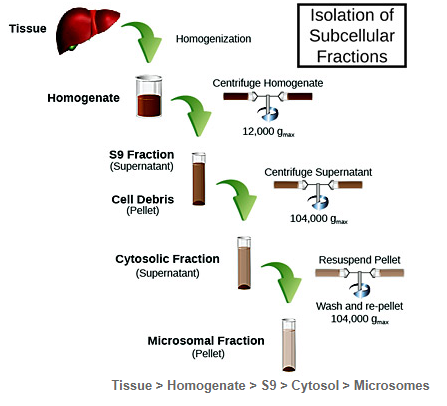
\includegraphics[width=1\linewidth]{media-04/image21} 

}

\caption{준세포분획(subcellular fraction)}\label{fig:04-03}
\end{figure}



\begin{figure}

{\centering 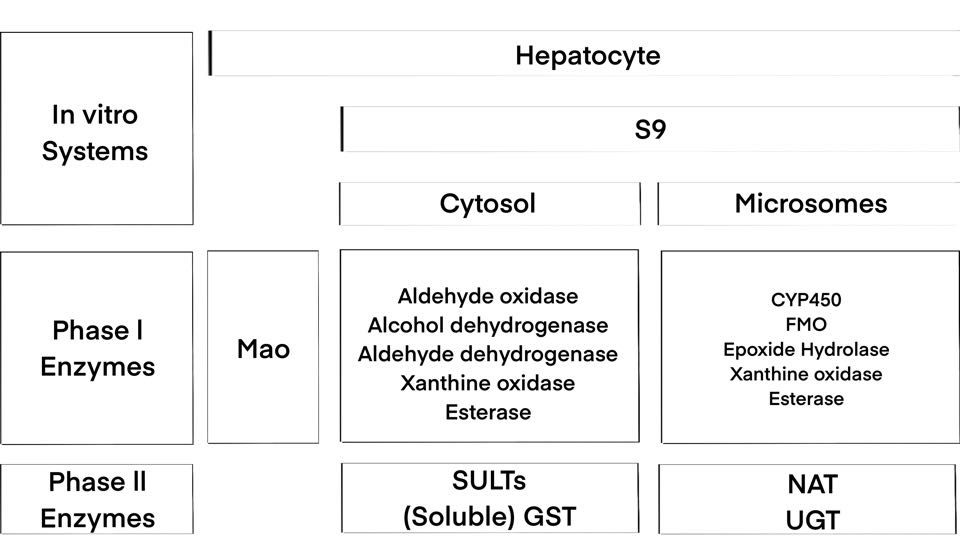
\includegraphics[width=1\linewidth]{media-04/image22} 

}

\caption{각 준세포분획(subcellular fraction)에 발현되어 있는 대사효소}\label{fig:04-04}
\end{figure}



\hypertarget{recombinant-enzyme}{%
\subsubsection{Recombinant enzyme}\label{recombinant-enzyme}}

재조합효소(recombinant enzyme)는 특정 대사효소를 인위적으로 과발현시켜
만든 실험계이다. 약물이 특정 대사효소로 얼마나 대사되는가를 평가할
때(reaction phenotyping study) 주로 사용된다. CYP 동효소 뿐만 아니라,
UGT 동효소, SULT, CES 등 다양한 재조합효소를 판매하고 있으며, 필요에
따라 실험자가 직접 과발현시킨 재조합효소를 만들어 실험에 사용할 수도
있다. 다만, 동일한 재조합효소의 농도를 실험에 사용하였더라도, 효소의
양과 활성은 재조합효소를 만들어내는 실험방법 및 상용화된 재조합효소를
판매하는 제조사마다 다르기 때문에, 필요에 따라 환산계수를 반영하여
CL\textsubscript{int}를 산출하여야 한다.

\hypertarget{uxb300uxc0acuxd3c9uxac00-uxc2e4uxd5d8uxc744-uxd1b5uxd574-uxc5bbuxc744-uxc218-uxc788uxb294-in-vitro-uxb300uxc0ac-uxd30cuxb77cuxbbf8uxd130}{%
\section{대사평가 실험을 통해 얻을 수 있는 in vitro 대사 파라미터}\label{uxb300uxc0acuxd3c9uxac00-uxc2e4uxd5d8uxc744-uxd1b5uxd574-uxc5bbuxc744-uxc218-uxc788uxb294-in-vitro-uxb300uxc0ac-uxd30cuxb77cuxbbf8uxd130}}

대사평가 실험을 통해 얻을 수 있는 in vitro 파라미터는 CL\textsubscript{int} 또는 K\textsubscript{m}
및 V\textsubscript{max}이다. 각 파라미터들은 다음과 같은 방법으로 얻을 수 있다.

\hypertarget{substrate-depletion-uxbc95}{%
\subsection{Substrate-depletion 법}\label{substrate-depletion-uxbc95}}

In vitro 대사평가 실험에서 시간에 따른 기질약물의 소실량을 측정하는
방법이다. 그림 \ref{fig:04-05}에서와 같이, 시간에 따라 기질 약물의 농도가
감소한다면, 실험계에 사용된 대사 효소의 기질임을 알 수 있다. 예를 들어,
microsome에 NADPH를 첨가하여 실험을 진행하였다면, 시험약물은 ES,
carboxylesterase (CES), CYP, FMO 등의 기질일 가능성이 높으며, 재조합
CYP3A4에서 아래의 결과를 얻었다면, 시험약물은 CYP3A4의 기질이다. 또한,
hepatocyte에서 실험 후, 아래의 결과를 얻었다면, 시험약물은 간에서
대사되는 약물이다. 이런 식으로, 실험 목적에 맞게 in vitro system을
선택하여 실험 후, 시험물질의 대사를 확인할 수 있다.

\begin{figure}

{\centering 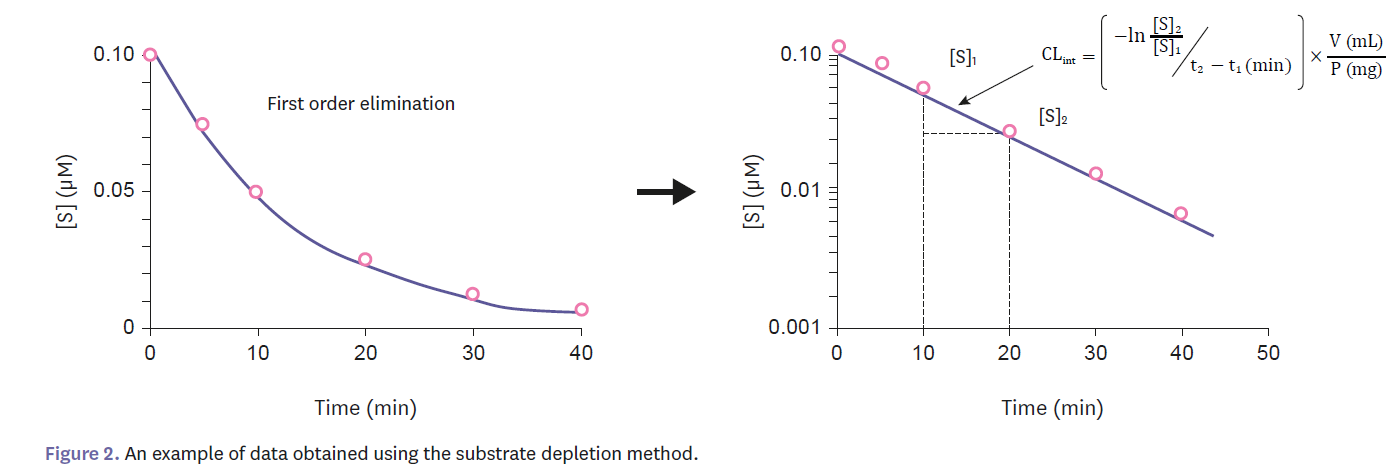
\includegraphics[width=1\linewidth]{media-04/image23} 

}

\caption{Substrate-depletion 법을 이용하여 얻을 수 있는 data (예)}\label{fig:04-05}
\end{figure}



Substrate-depletion 법을 통해서, 어떤 대사효소로 대사되는지 확인할 수
있을 뿐만 아니라, 얼마나 대사되는지도 확인할 수 있다. 시간에 따른
기질약물의 소실속도가 일차반응속도를 따른다면, y축을 log로 변환하면 그림 \ref{fig:04-05}의 오른쪽과 같이, 그래프가 직선을 나타낸다. 이때의 기울기는
제거속도상수(k)이며, 여기에 실험에 사용된 buffer의 양(mL)과 실험에
사용된 단백질의 양(mg)을 반영하면, CL\textsubscript{int}를 구할 수 있다.

\begin{equation}
CL_{int} = \frac{-ln\frac{[S]_2}{[S]_1}}{t2 - t1 \text{ (min)}} \cdot \frac{V\text{ (ml)}}{P\text{ (mg)}}
\label{eq:eq04-01} 
\end{equation}

이 때, 기질은 K\textsubscript{m} 이하의 농도를 선택하는 것이 중요하다. 대부분의
기질-효소 반응은 Michaelis -Menten (M-M) kinetic을 따르며, K\textsubscript{m} 이하의
저농도에서는 1차반응, K\textsubscript{m} 이상의 고농도에서는 0차 반응을 보인다.
Substrate-depletion 법은 약물의 대사속도를 일차반응속도로 가정하고 있기
때문에, 정확한 CL\textsubscript{int}를 구하기 위해서는 저농도를 기질의 농도로 선택하여
실험하여야 한다. 하지만, 신약개발 초기단계의 경우, 어떤 대사효소에 의해
얼만큼 대사되는지에 대한 정보가 없어 기질의 특정효소에 대한 K\textsubscript{m}값을 알
수 없으므로, 기질 농도는 정량가능한 범위에서 최대한 낮은 농도를 선택하는
것이 좋다. 높은 농도에서 substrate-depletion법을 통해 CL\textsubscript{int}를
산출하였다면, 그 약물의 대사능이 underprediction 될 수 있다.

\hypertarget{metabolite-formation-uxbc95}{%
\subsection{Metabolite-formation 법}\label{metabolite-formation-uxbc95}}

대사체를 정량분석기기(LC-MS/MS 등)를 통해 정량적으로 농도 분석할 수
있다면, 기질 약물농도에 따른 대사체 생성량을 측정할 수 있다. 그림 \ref{fig:04-06}처럼, 기질-효소 반응은 M-M kinetic을 통해 대사체를 생성하며,
기질농도에 따라 대사효소의 포화 등으로 인해 대사체 생성 속도가 달라질 수
있다. Metabolite-formation 법을 통해 시험물질을 대사시키는 대사효소를
특정할 수 있으며, substrate-depletion 법과 달리 기질 농도에 따른 대사체
생성속도를 확인하기 때문에, 대사효소에 대한 시험물질의 V\textsubscript{max}와 K\textsubscript{m}을
산출할 수 있다. 실험계는 간세포, 준세포분획, 재조합효소 등 실험목적에
맞게 다양하게 선택할 수 있다. Metabolite-formation 법을 통한 대사평가는
주대사체(major metabolite)가 생성되거나, 대사체에 대한 구조확인
시험물질의 대사체 표준품(표준시료)이 확보되어야 하기 때문에, 신약
개발단계에서 metabolite profiling을 통한 대사체 동정 이후에 수행되는
경우가 일반적이다.

\begin{figure}

{\centering \includegraphics[width=1\linewidth]{media-04/image25} 

}

\caption{Metabolite-formation법을 이용하여 얻을 수 있는 data (예)}\label{fig:04-06}
\end{figure}



\hypertarget{uxb300uxc0acuxd3c9uxac00-uxc2e4uxd5d8uxbc95}{%
\section{대사평가 실험법}\label{uxb300uxc0acuxd3c9uxac00-uxc2e4uxd5d8uxbc95}}

약물 대사 평가 방법에 대하여 알아보자. 평가하고자 하는 대사효소가
포함되어 있는 실험계를 선택할 수 있다.

\hypertarget{uxb300uxc0acuxc548uxc815uxc131metabolic-stability-uxd3c9uxac00-uxc2e4uxd5d8}{%
\subsection{대사안정성(metabolic stability) 평가 실험}\label{uxb300uxc0acuxc548uxc815uxc131metabolic-stability-uxd3c9uxac00-uxc2e4uxd5d8}}

신약개발 시 후보물질 도출을 위한 초기 단계에 많이 활용된다. 일반적으로
microsome을 이용하지만, 평가하고자 하는 목적에 따라 다른 실험계를 선택할
수 있다. Microsome을 이용할 경우, 첨가하는 cofactor와 chemical inhibitor
종류 및 pre-incubation 조건에 따라 다양한 효소의 대사능을 선택적으로
관찰할 수 있다. 각 실험 조건에 맞게 약물이 들어있는 튜브를 준비하여,
37℃에서 incubation 하면서 시간에 따라 tube내의 약물의 농도를 측정하여
tube에서 사라지는(대사되는) 약물의 양을 확인한다. 표 \ref{tab:table04-04}를 자세히
살펴보자. G1은 평가약물과 buffer만 있으므로, 약물이 실험에 사용되는
buffer에서 chemical degradation이 있는지 확인하는 대조군이다. G2는
buffer와 microsome을 포함하고 있으며, cofactor 없이 가수분해가 가능한 ES
및 CES에 의한 대사를 관찰할 수 있다. G3은 G2에 NADPH를 추가하였으며, 이
경우는 가수분해효소 외 CYP와 FMO에 의한 대사를 관찰할 수 있다. G4는 G2에
NADPH 대신 UDPGA (+alamethicin)을 첨가하였으며, 이는 UGT에 의한 대사를
관찰하기 위함이다. G1\textasciitilde G4의 조건은 대사안정성 실험시 필수적으로 포함하여
수행하기를 권장하며, 여기에 더하여, FMO 대사 가능성이 있다면, G5와 G6
실험을 추가하는 것을 추천한다. G5는 45℃에서 30분가 pre-incubation하여
열에 약한 microsome 내의 FMO를 비활성화 시키게 되며, G6는 CYP 동효소의
chemical inhibitor인 SKF525A를 첨가하여, CYP에 의한 대사능을 배제시킬 수
있다.

\begin{longtable}[]{@{}
  >{\raggedright\arraybackslash}p{(\columnwidth - 12\tabcolsep) * \real{0.1806}}
  >{\raggedright\arraybackslash}p{(\columnwidth - 12\tabcolsep) * \real{0.1250}}
  >{\raggedright\arraybackslash}p{(\columnwidth - 12\tabcolsep) * \real{0.1250}}
  >{\raggedright\arraybackslash}p{(\columnwidth - 12\tabcolsep) * \real{0.1250}}
  >{\raggedright\arraybackslash}p{(\columnwidth - 12\tabcolsep) * \real{0.1250}}
  >{\raggedright\arraybackslash}p{(\columnwidth - 12\tabcolsep) * \real{0.1250}}
  >{\raggedright\arraybackslash}p{(\columnwidth - 12\tabcolsep) * \real{0.1250}}@{}}
\caption{\label{tab:table04-04} 대사안정성 평가 실험법의 예}\tabularnewline
\toprule()
\begin{minipage}[b]{\linewidth}\raggedright
\end{minipage} & \begin{minipage}[b]{\linewidth}\raggedright
\textbf{G1}
\end{minipage} & \begin{minipage}[b]{\linewidth}\raggedright
\textbf{G2}
\end{minipage} & \begin{minipage}[b]{\linewidth}\raggedright
\textbf{G3}
\end{minipage} & \begin{minipage}[b]{\linewidth}\raggedright
\textbf{G4}
\end{minipage} & \begin{minipage}[b]{\linewidth}\raggedright
\textbf{G5}
\end{minipage} & \begin{minipage}[b]{\linewidth}\raggedright
\textbf{G6}
\end{minipage} \\
\midrule()
\endfirsthead
\toprule()
\begin{minipage}[b]{\linewidth}\raggedright
\end{minipage} & \begin{minipage}[b]{\linewidth}\raggedright
\textbf{G1}
\end{minipage} & \begin{minipage}[b]{\linewidth}\raggedright
\textbf{G2}
\end{minipage} & \begin{minipage}[b]{\linewidth}\raggedright
\textbf{G3}
\end{minipage} & \begin{minipage}[b]{\linewidth}\raggedright
\textbf{G4}
\end{minipage} & \begin{minipage}[b]{\linewidth}\raggedright
\textbf{G5}
\end{minipage} & \begin{minipage}[b]{\linewidth}\raggedright
\textbf{G6}
\end{minipage} \\
\midrule()
\endhead
Buffer & O & O & O & O & O & O \\
Microsomes & X & O & O & O & O & O \\
NADPH & X & X & O & X & O & O \\
UDPGA
(+ala-
methicin) & X & X & X & O & X & X \\
SKF525A & - & - & - & - & - & O \\
Pre-
incubation & 37℃,

5 min & 37℃,

5 min & 37℃,

5 min & Ice,

30 min & 45℃,

30 min & 37℃,

5 min \\
평가가능한
대사효소 & X & ES,
CES & ES,
CES,
CYP,
FMO & ES,
CES,
UGT & ES,
CES,
CYP & ES,
CES,
FMO \\
\bottomrule()
\end{longtable}

위의 방법을 통해 수행된 실험 결과는 그림 \ref{fig:04-07}와 같이 얻을 수 있다. 각
군에서 특정 대사효소에 의해 대사가 일어난 경우, 시간에 따라 약물의
농도가 줄어들기 때문에, 표 \ref{tab:table04-04}의 G6과 같은 결과가 나타나며, 그렇지
않은 경우는 시간에 따른 약물 농도의 변화가 관찰되지 않는다.
Substrate-depletion 법을 사용하기에, 시험물질의 농도는 가능한 낮은
농도에서 실험하기를 권장한다. 그리고 표 \ref{tab:table04-04}의 실험 조건들은 일반적으로
많이 사용되는 방법이며, 시험물질의 구조에 따라 대사가 일어날 가능성이
있는 대사효소를 평가할 수 있도록, 실험 조건을 적절히 변경하여 평가에
활용할 수 있다.

\begin{figure}

{\centering \includegraphics[width=1\linewidth]{media-04/image26} 

}

\caption{대사안정성 평가 실험 결과 (예)}\label{fig:04-07}
\end{figure}



\hypertarget{reaction-phenotyping-uxd3c9uxac00-uxc2e4uxd5d8}{%
\subsection{Reaction phenotyping 평가 실험}\label{reaction-phenotyping-uxd3c9uxac00-uxc2e4uxd5d8}}

Reaction phenotyping 실험은 일반적으로 metabolic stability 실험 후에
수행한다. 이 실험은 특정 대사효소계에 의해 대사됨을 확인한 후, 그 중에
특정한 대사효소를 찾아내기 위함이다. 예를 들어, 대사안정성 실험을 통해
시험물질이 CYP 동효소에 의해 대사됨을 확인하였다면, 그 이후에 reaction
phenotyping 실험을 통해 CYP 동효소 중에서 어떠한 효소로 대사되는지 특정
대사효소를 찾아낼 수 있다. 이 뿐만 아니라, total in vivo CL 중에서 특정
대사효소에 의해 대사되는 정도(기여도) (i.e., the fraction of drug
metabolized by a specific enzyme, f\textsubscript{m})를 확인할 수 있다. CYP에 의한
약물 대사가 total in vivo CL의 25\% 이상을 차지하면, 특정 CYP 효소를
확인(identification)하는 것이 권장된다{[}Studies (\protect\hyperlink{ref-studies2020cytochrome}{2020})\}. Reaction phenotyping
평가에는 1) recombinant enzymes (i.e.~CYP 동효소, UGT 동효소 등) 이용,
2) enzyme-selective chemical inhibitors or antibodies 이용 등의 실험법이
사용될 수 있으며, 미국 FDA는 1)과 2)의 방법을 모두 사용하기를 권고하고
있다{[}Studies (\protect\hyperlink{ref-studies2020cytochrome}{2020})\}.

재조합효소를 사용하는 실험법은 시험물질의 구조와 metabolic stability
자료를 바탕으로 수행될 수 있다. CYP 동효소들, UGT 동효소들, MAO, FMO,
CES 등 대사 가능성이 있는 모든 효소에 대하여 확인할 수 있으며,
substrate-depletion 방법과 metabolite-formation 방법 둘 다 사용
가능하다.

Recombinant CYP 동효소를 이용한 reaction phenotyping의 예를
살펴보자(그림 \ref{fig:04-08}, \ref{fig:04-09}, \ref{fig:04-10}). 그림 \ref{fig:04-08}에서와 같이, 재조합 CYP 동효소 각각에
시험물질을 넣고 일정시간동안 incubation 후, 시험물질의 소멸양을 확인하여
특정 대사효소를 찾아낼 수 있다. 생성 대사체에 대한 정보가 없다면, 이와
같은 방법을 사용할 수 있다. 그림 \ref{fig:04-08}의 결과에서는 실험에 사용된 물질은
주로 CYP3A4와 CYP3A5를 통해 대사됨을 확인할 수 있다.

\begin{figure}

{\centering \includegraphics[width=1\linewidth]{media-04/image27} 

}

\caption{Recombinant CYP 동효소를 이용한 reaction phenotyping 예 (substrate-depletion method). rCYP, recombinant CYP; HLM, human liver microsome}\label{fig:04-08}
\end{figure}



대사체의 분자량과 LC-MS/MS 분석조건을 알고 있다면, 그림 \ref{fig:04-09}에서와 같이
각 CYP 동효소를 통해 생성되는 대사체를 확인할 수 있다. 이 경우, 대사체의
절대 생성량을 측정한 것이 아니라, 분석기기에서 생성된 대사체의 peak
면적을 확인한 것이므로, y축이 relative intensity임을 참고하자.

\begin{figure}

{\centering \includegraphics[width=1\linewidth]{media-04/image28} 

}

\caption{Recombinant CYP 동효소를 이용한 reaction phenotyping 예 (metabolite-formation method) (\protect\hyperlink{ref-yanakakis2012biotransformation}{Yanakakis and Bumpus 2012}). 각 CYP 동효소를 이용해 생성되는 대사체의 상대량(relative intensity)를 확인할 수 있다.}\label{fig:04-09}
\end{figure}



대사체의 표준품을 이용한 검량선 작성이 선행되어야 정확한 생성량과 관련된
파라미터들을 알 수 있다. 이의 예는 그림 \ref{fig:04-10}에 잘 나와 있다. 시험물질의
CYP3A4에 의해 대사되어 생성되는 대사체인 M1과 M2의 생성량을 기질 약물의
농도에 따라 확인하였으며, 이를 통해 특정 대사효소에 의해 생성되는 특정
대사체의 생성을 설명하는 파라미터인 K\textsubscript{m}과 V\textsubscript{max}를 얻을 수 있다. 이를
통해, 시험물질의 대사능을 정량적으로 확인할 수 있으며 (K\textsubscript{m}, V\textsubscript{max},
CL\textsubscript{int}), 이를 통해 f\textsubscript{m}을 계산할 수 있다. 여기서 한가지 주의할 점은,
재조합효소를 이용하여 정량적인 값(CL\textsubscript{int})을 산출하고, 이를 \emph{in vitro} -
\emph{in vitro} extrapolation (IVIVE)를 통해 in vivo CL 계산에 활용하고자 할
때에는 ISEF 또는 RAF 등의 적절한 환산계수를 반영하여야 한다.

\begin{figure}

{\centering \includegraphics[width=1\linewidth]{media-04/image29} 

}

\caption{Recombinant CYP 동효소를 이용한 reaction phenotyping 예 (metabolite-formation method) (\protect\hyperlink{ref-yanakakis2012biotransformation}{Yanakakis and Bumpus 2012}). 대사체의 표준품 확보가 가능한 경우}\label{fig:04-10}
\end{figure}



\hypertarget{uxb9fauxc74cuxb9d0-3}{%
\section{맺음말}\label{uxb9fauxc74cuxb9d0-3}}

신약개발 과정에서 in vitro 약물대사를 평가 실험은 필수적이다. 임상진입
전, 후보물질의 대사 특성을 잘 파악하고 질 높은 정량적인 파라미터들을
확보해 두는 것은 임상개발 과정에서 시간과 비용을 줄이는데 중요한 역할을
할 수 있다. 대사 평가 데이터는 임상진입을 위한 허가기관 제출 자료로
확보되어야 하며, 그 외, 임상 진입 후, PBPK 모델 개발에 필수적으로
활용되어, 병용약물과의 약동학적 상호작용 평가, 다양한 환자군(예. 간 및
신장 기능 저하 환자군, 등)에서의 약동학 평가, 및 인종간의 약동학 차이
등의 평가에 사용될 수 있다.

\hypertarget{uxd6c4uxbcf4-uxbb3cuxc9c8uxc758-uxb300uxc0ac-uxc5b5uxc81c-uxd2b9uxc131-uxd3c9uxac00}{%
\chapter{후보 물질의 대사 억제 특성 평가}\label{uxd6c4uxbcf4-uxbb3cuxc9c8uxc758-uxb300uxc0ac-uxc5b5uxc81c-uxd2b9uxc131-uxd3c9uxac00}}

이소진

\hypertarget{uxac1cuxc694}{%
\section{개요}\label{uxac1cuxc694}}

이 장에서는 개발하는 약물이 과연 inhibitor 역할을 하는 약물인지
확인하고, 어떤 inhibition 특성을 가지는지 확인하는 방법을 살펴보기로
한다. Inhibition의 종류는 크게 두가지로 분류되며, Reversible inhibition
과 Time-dependent inhibition으로 나뉜다. 각각의 inhibition 종류에 따른
inhibition assay 실험 방법과 이를 통해 얻은 데이터를 해석하는 방법,
그리고 이 정보를 DDI prediction에 적용하는 방법에 대해 살펴보겠다.

DDI 평가는 중요하며, 특히 여러 종류의 약물을 장기간 병용 투약하는
만성질환을 가진 환자에서 조심해야한다. Inhibitior 역할을 하는 약물은
victim drug 와 병용투여시 victim drug의 체내 약물 농도를 높게 만들고,
이에 따른 이상반응이나 독성이 나타날 수 있다. DDI 평가는 in vitro ADME
study 시작에서부터 함께 탐색되는 것을 추천한다. 이와 같은 in vitro
단게에서의 DDI 평가는 FDA 가이던스와 EMA 가이드 라인에서도 추천되어
진다.

\includegraphics[width=2.59167in,height=1.68983in]{./media/image1.emf}\includegraphics[width=2.70547in,height=1.69792in]{./media/image2.png}

그림 . Perpetrator(inhibitor 또는 inducer) 와 victim drug 병용투여 시의
약물농도

Victim (substrate) : Drug whose PK is affected
Perpetrator : Drug that is affecting PK of victim

\hypertarget{Induction}{%
\chapter{후보 물질의 대사 유도 특성 평가}\label{Induction}}

\Large\hfill

최수인
\normalsize

\hypertarget{uxc11cuxb860-4}{%
\section{서론}\label{uxc11cuxb860-4}}

대사 유도란 주로 약이나 화학물질에 의해서 효소의 대사 능력이 증가하는 현상을 말한다. 특히 약동학적 약물상호작용 측면에서는 이러한 대사 유도의 양이 많아져서 기질의 청소율이 증가하는 것을 의미한다.
따라서 유도체(inducer)란 특정 효소를 이러한 방식으로 유도할 수 있는 능력이 있는 물질을 말한다.
유도체에 의해 대사 효소가 증가하게 되면 이에 따라 기질의 청소율이 증가하게 되며 이는 기질의 인체에서의 노출 감소 또는 기질의 대사체의 노출 증가를 일으키며 이로 인해 약의 효능과 안전성 모두 영향을 미칠 수 있다.
대사 유도에 의한 영향은 capacity가 낮은 CYP isoform에서 특히 더 나타나게 된다. CYP isoform이 아닌 효소에서도 유도 현상이 나타날 수 있으나 이러한 효소들은 대부분 친화도(affinity)가 낮고 capacity가 높기 때문에 기질의 청소율에 큰 영향을 미치는 경우는 드물다.
유도체는 대사효소의 생성 속도를 증가시키거나 대사 효소의 안정화를 통해 반감기를 감소시켜 대사 효소의 숫자를 증가시킨다.
종간 차이가 크며 이러한 효소양의 변화는 시간에 따라 변화하며 생성속도 혹은 감소속도를 변화시키기 때문에 유도 효과가 나타나기 까지는 비교적 다른 약물상호작용에 비해 긴 시간이 걸리며 (7\textasciitilde10일) 특히 복용을 멈춰도 이러한 현상은 당분간은 유지된다. CYP isoform의 경우는 이러한 청소율의 변화가 매우 크게 나타날 수 있다.

유도 현상의 대표적인 예는 알코올 중독 환자의 아세트아미노펜 복용, 항간질약과

\hypertarget{uxc720uxb3c4uxccb4uxc758-uxc791uxc6a9-uxba54uxcee4uxb2c8uxc998}{%
\section{유도체의 작용 메커니즘}\label{uxc720uxb3c4uxccb4uxc758-uxc791uxc6a9-uxba54uxcee4uxb2c8uxc998}}

일반적으로 유도체는 위 그림\ref{fig:mechanism}과 같이 Nucleus의 Receptor와의 결합을 통해 유전자의 전사를 유도하여 효소의 생성을 증가 시킨다.
작용 메커니즘은 비슷하나 CYP isoform에 따라서 크게 3가지의 Nucleus receptor가 관여하게 된다.

\begin{longtable}[]{@{}
  >{\raggedright\arraybackslash}p{(\columnwidth - 4\tabcolsep) * \real{0.3143}}
  >{\raggedright\arraybackslash}p{(\columnwidth - 4\tabcolsep) * \real{0.3143}}
  >{\raggedright\arraybackslash}p{(\columnwidth - 4\tabcolsep) * \real{0.3714}}@{}}
\toprule()
\begin{minipage}[b]{\linewidth}\raggedright
유도 메커니즘
\end{minipage} & \begin{minipage}[b]{\linewidth}\raggedright
CYP isoform
\end{minipage} & \begin{minipage}[b]{\linewidth}\raggedright
특징
\end{minipage} \\
\midrule()
\endhead
AhR (Aryl hydrocarbon receptor) mediated control & CYP1A1, CYP1A2, CYP1B1 & 수용체와의 결합은 주로 세포질에서 일어나며 결합체가 Nucleus 안으로 이동하여 유전자 전사를 증가시킴. 모든 조직에 분포해 있으며 CYP 효소 외에도 NADPH reductase, glutathion S-transference, Aldehyde dehydrogenase의 생성에도 관여하기 때문에 조직의 발달에 영향을 미칠 수 있음 \\
CAR (Constitutive androstane receptor) mediated control & CYP2B6, CYP2C9, CYP3A4 & 주로 핵내에서 결합하며 결합한 수용체는 해당 수용체의 expression 정도가 사람간의 차이가 커서 유도능력의 차이를 일으킴. \\
물리화학적 특성 & 규명이 쉬움 & 복잡한 특성 \\
정량적 측정 방법 & 잘 확립되어 있음 (LC-MS/MS) & 정량 분석 품질 낮음 (ELISA, LC-MS/MS) \\
\textbf{생리학적 특성} & & \\
흡수 & 세포막 투과 쉽고 위장관 흡수 좋음 & 세포막 투과 어렵고 위장관 투여 불가능 \\
분포 & 혈관 외 조직으로의 분포가 크게 나타날 수 있음, 혈장 및 조직에서의 단백 결합에 영향을 받음. 장기 분포 ∝ 조직 친화성 & 혈관 외 분포가 적고 단백 결합은 고려하지 않음. 장기 분포 ∝ 혈관 투과도와 수용체 분포정도 \\
대사 & Phase I/II 대사로 인한 다른 물질로 변환 & 펩타이드/아미노산으로 분해 \\
배설 & 담즙 또는 소변 배설. 궁극적인 제거 경로 & 거의 배설되지 않음 \\
면역유발 & 흔치 않음. 과민반응 형태의 독성 작용 & 비교적 흔함. 항약물항체(ADA)에 의해 약물 제거될 수 있음 \\
\bottomrule()
\end{longtable}

\hypertarget{uxd2b9uxc9d5}{%
\subsection{특징}\label{uxd2b9uxc9d5}}

유도체의 작용은 주로 Receptor와의 결합을 통해 해당 효소의 유전자의 전사가 증가되는 것으로 전사 이후에도 효소 단백질이 만들어지기 까지는 일련의 과정을 거치게 되기 때문에 실제로 효소 단백질이 증가되는 과정은 과정에 따라 짧게는 며칠, 길게는 몇주까지로 매우 느리다. 또한 유전자의 전사를 증가시키는 과정을 하기 때문에 단순한 효소 단백질의 증가로 인한 대사의 증가 외에 다른 potential한 변화가 더 크게 나타날 수 있다.
해당 과정은 가역적이나 기존의 형태로 돌아가기에는 비교적 느리다. 효소 단백질의 생성 속도는 전사 속도가 증가할 수록 증가하게 된다.
이러한 생성 속도의 증가로 인해서 유도체의 작용이 일정할 때 효소 단백질의 양은 새로운 평형에 도달하게 되며 해당 과정은 주로 효소 단백질 고유의 반감기에 의해 좌우된다.

\hypertarget{uxc720uxb3c4uxccb4uxc5d0-uxc758uxd55c-uxd65cuxc131uxd6a8uxc18cuxc758-uxbcc0uxd654}{%
\subsection{유도체에 의한 활성효소의 변화}\label{uxc720uxb3c4uxccb4uxc5d0-uxc758uxd55c-uxd65cuxc131uxd6a8uxc18cuxc758-uxbcc0uxd654}}

효소는 체내에서 평형을 이루고 있으며 아래 그림과 같이 일정한 생성속도와 제거속도에 의해 결정되는 turnover model을 따른다(그림 \ref{fig:turnover}). turnover model을 표현한 식은 아래 식\eqref{eq:eq10-1}과 같으며 유도체가 없는 상황에서는 생성속도(R\textsubscript{syn})와 제거속도(k\textsubscript{deg} * Enz(0))가 동일한 동적 평형 상태(\(\frac{dEnz(t)}{dt}\))를 이룬다.

\begin{verbatim}
## Error in knitr::include_graphics("media-07/turnover.png"): Cannot find the file(s): "media-07/turnover.png"
\end{verbatim}



\begin{equation}
\frac{dEnz(t)}{dt} = R{syn} - k{deg} \cdot Enz(t)
\label{eq:eq10-1} 
\end{equation}

유도체는 수용체와의 결합을 통해 효소 mRNA의 전사 속도를 증가시키기 때문에 해당 식의 생성속도(R\textsubscript{syn})를 증가시키는 것으로 볼 수 있다. 이러한 생성속도의 증가 정도는 유도체의 유도 능력(E\textsubscript{50}, E\textsubscript{max})과 농도에 영향을 받게 되기 때문에 일반적으로 아래의 식\eqref{eq:eq10-2}과 같이 유도로 인한 생성속도의 증가를 표현한다.

\begin{equation}
\frac{dEnz(t)}{dt} = R{syn} \cdot (1 + \frac{E{max}C(t)}{EC{50} + C(t)}) - k{deg} \cdot Enz(t)
\label{eq:eq10-2}
\end{equation}

단, 예외적으로 CYP2E1의 경우, 유도체는 효소의 안정화를 일으키므로 제거속도(k\textsubscript{deg})를 감소시키는 방향으로 작용한다.

\hypertarget{uxd6c4uxbcf4-uxbb3cuxc9c8uxc758-uxc720uxb3c4-uxac00uxb2a5-uxc5ecuxbd80-uxd3c9uxac00uxb97c-uxc704uxd55c-in-vitro-study-uxb514uxc790uxc778}{%
\section{후보 물질의 유도 가능 여부 평가를 위한 In vitro study 디자인}\label{uxd6c4uxbcf4-uxbb3cuxc9c8uxc758-uxc720uxb3c4-uxac00uxb2a5-uxc5ecuxbd80-uxd3c9uxac00uxb97c-uxc704uxd55c-in-vitro-study-uxb514uxc790uxc778}}

후보 물질의 유도체로써의 작용 가능성과 작용 정도에 대한 평가는 대부분 해당 물질의 개발 과정에 따라 다르게 이루어진다.
기본적으로 초기 개발 단계의 경우 스크리닝을 위한 assay가 이뤄지며 주로 96-well plated HHEP 방법이 사용된다. 이 방법은 물질의 구체적인 약동학 정보가 나오기 전에 유도체로서의 가능성 정도를 타진해 보고자 수행되기 때문에 3\textasciitilde4가지의 정해진 농도로 2\textasciitilde3일 정도 처리해서 mRNA 또는 enzyme의 fold change 정도를 확인한다. CYP3A4는 CYP2C9 및 CYP2B6와 작용하는 수용체와 메커니즘이 유사하기 때문에 스크리닝 단계에서는 주로 CYP3A4 에 대해서만 시험하게 된다.

후보 물질의 개발 단계가 진행되면서 유도체로써의 작용에 대한 세밀한 평가가 이루어지게 된다. 이 경우는 3명 이상의 사람 간세포를 주로 이용하며 음성 대조군과 양성 대조군이 모두 사용된다. 양성 대조군으로는 주로 rifampin 을 사용하나 평가되는 효소에 따라 다른 물질일 사용될 수 있다. 이 단계에서 주로 RT-PCR을 이용하여 vehicle control 대비 증가한 mRNA의 fold change 크기를 통해 유도 능력을 평가한다. mRNA가 아닌 활성화된 효소의 fold change의 경우 약물의 억제 작용이 혼재되어 나타날 수 있기 때문에 잘 선호되지 않으나 CYP1E2에 대한 유도 가능성이 있는 경우 효소의 안정화를 확인해야 하기 때문에 enzyme을 측정하게 된다.
유도체의 경우 주로 3일 이상 관찰하며 사용하는 농도는 약물의 용해도, 간세포에 대한 독성과 약동학 정보를 고려하여 결정한게 된다. 특히 예측되는 인체 내 최대 노출 정도 (C\textsubscript{max,u})에 대한 30\textasciitilde50배 값을 이용하게 된다. 유도체에 대한 시험이 끝나면 세포 독성을 확인하게 되며 만약 3일 이상 세포가 살아있지 않으면 관찰 기간을 축소하거나 조금 더 낮은 농도를 사용하게 된다.
집단내에서 CYP발현 정도와 반감기 등은 사람간 차이가 있기 때문에 유도 결과 역시 donor에 따라 다르게 나타날 수 있으며 assay environment에 따라도 다르게 나타난다.

\hypertarget{uxc57duxbb3c-uxc218uxc1a1uxccb4uxc5d0-uxb300uxd55c-uxd6c4uxbcf4uxbb3cuxc9c8uxc758-uxc791uxc6a9uxd3c9uxac00}{%
\chapter{약물 수송체에 대한 후보물질의 작용평가}\label{uxc57duxbb3c-uxc218uxc1a1uxccb4uxc5d0-uxb300uxd55c-uxd6c4uxbcf4uxbb3cuxc9c8uxc758-uxc791uxc6a9uxd3c9uxac00}}

\Large\hfill

배수현
\normalsize

\hypertarget{uxc11cuxb860-5}{%
\section{서론}\label{uxc11cuxb860-5}}

세포내 물질 이동은 그림 \ref{fig:07-01}과 같다. 크게 수동수송과 능동수송으로 구분할
수 있다. 수동수송은 세포막 사이의 물질의 농도 차이에 의해 발생한다. 즉,
물질의 농도가 높은 곳에서 낮은 곳으로 농도 구배에 따라 이동하며,
에너지를 사용하지 않는다. 비극성 물질은 단순확산(passive diffusion)
되며, 극성을 띄는 물질은 촉진 확산(facilitated diffusion)을 통해
세포막을 통과한다. 반면, 능동수송은 물질이 농도에 역행하여 이동하며
이때, 에너지를 사용한다. 낮은 농도에서 높은 농도로 물질이 이동하기
때문에 지속적으로 에너지를 사용하게 되며, 수송체를 통해 물질이 이동한다.
수송체의 종류에 따라 Solute carrier (SLC) transporter와 ATP-binding
cassette (ABC) transporter로 나뉜다. 이 단원에서는 약물을 세포 내외로
이동시키는데 관여하는 수송체의 종류와 특성을 살펴보고, 신약후보물질의
수송체 기질 및 저해능 평가 방법에 대하여 기술한다.

\begin{figure}

{\centering \includegraphics[width=1\linewidth]{media-07/image1} 

}

\caption{세포내 물질의 이동 원리}\label{fig:07-01}
\end{figure}



\hypertarget{uxc57duxbb3cuxc218uxc1a1uxccb4uxc758-uxc885uxb958uxc640-uxc5eduxd560}{%
\section{약물수송체의 종류와 역할}\label{uxc57duxbb3cuxc218uxc1a1uxccb4uxc758-uxc885uxb958uxc640-uxc5eduxd560}}

약물 수송체의 종류는 크게 SLC transporter와 ABC transporter로 나뉜다.
SLC 수송체는 주로 세포내로 물질을 수송(uptake)시키며, 나트륨(Na+) 등의
매개물질을 이용하여 물질을 함께 이동시키기도 한다. 이 경우, 매개물질이
농도 구배에 역행하여 에너지를 사용하며 이와 함께 물질이 이동하게 되므로
2차 수송이라고도 하며, 이온과 같은 방향으로 물질이 이동하는
경우(symport)와 다른 방향으로 물질이 이동하는 경우(antiport)가 있다.
전하를 띄고, 친수성 물질, 분자량이 작을수록 SLC 수송체의 기질일 가능성이
높다.

ABC 수송체는 SLC 수송체와 반대로, 주로 물질을 세포밖으로
수송(efflux)시킨다. 물질이 직접 농도 구배에 역행하여 수송되면서 ATP를
사용한다. 분자량이 상대적으로 크며, 지용성 물질 등이 기질인 경우가 많다.

다양한 종류의 수송체가 세포 표면에 분포하고 있으며, 이 중 약물의 ADME에
영향을 주는 수송체의 종류는 표 \ref{tab:transporter}에 정리되어 있다.



\begin{table}

\caption{\label{tab:transporter}약물 수송체의 종류}
\centering
\begin{tabular}[t]{lllll}
\toprule
Gene & Aliases & Tissue & Substrate & Inhibitor\\
\midrule
ABCB1 & P-gp, MDR1 & intestine, liver, kidney, brain, placenta, adrenal, testes & digoxin, fexofenadine, indinavir, vincristine, colchicine, topotecan, paclitaxel, loperamide, doxorubicin, vinblastine & ritonavir, cyclosporine, verapamil, erythromycin, ketocoanzole, itraconazole, quinidine, elacridar (GF120918), LY335979, valspodar (PSC833)\\
ABCB4 & MDR3 & liver & digoxin, paclitaxel, vinblastine & verapamil, cyclosporine\\
ABCB11 & BSEP & liver & pravastatin, taurocholic acid, bile acids & cyclosporine, rifampicin, glibenclamide\\
ABCC1 & MRP1 & intestine, liver, kidney, brain & adefovir, indinavir & \\
ABCC2 & MRP2, CMOAT & intestine, liver, kidney, brain & methotrexate, glucuronides, valsartan, indinavir, cisplatin, & cyclosporine, delavirdine, efavirenz, emtricitabine\\
\addlinespace
ABCC3 & MRP3, CMOAT2 & intestine, liver, kidney, placenta, adrenal & etoposide, methotrexate, tenoposide, glucoronides, fexofenadine & delavirdine, efavirenz, emtricitabine\\
ABCC4 & MRP4 & liver, brain & adeforvir, tenofovir, methotrexate, topotecan, furosemide, cAMP, & celecoxib, diclofenac\\
ABCC5 & MRP5 & brain &  & \\
ABCC6 & MRP6 & liver, kidney & cisplatin, daunorubicin & \\
ABCG2 & BCRP & intestine, liver, mammary glands, placenta & daunorubicin, doxorubicin, topotecan, rosuvastatin, sulfasalazine, imatinib, methotrexate & elacridar (GF120918), gefitinib, fumitremorgin C, novobiocin\\
\addlinespace
SLCO1A2 & OATP1A2, OATP-A & brain, liver, kidney & E3S, statins, fexofenadine, bile salts, digoxin, methotrexate & naringin, ritonavir, lopinavir, saquinavir, rifampicin\\
SLCO1B1 & OATP1B1, OATP- C, OATP2 & liver & rifampin, rosuvastatin, methotrexate, pravastatin, thyroxine, bilirubin, E17BG, & cyclosporine, rifampicin, saquinavir, ritonavir, lopinavir\\
SLCO1B3 & OATP1B3, OATP8 & liver & digoxin, fexofenadine, telmisartan, E17BG, bile acids, statins, & rifampicin, cyclosporine, ritonavir, lopinavir\\
SLCO2B1 & OATP2B1, OATP-B & intestine, liver, kidney, brain & E3S, statins, taurocholate, fexofenadine, glyburide & rifampicin, cyclosporine\\
SLC10A1 & NTCP & liver, pancreas & rosuvastatin, chlorambucil taurocholate & \\
\addlinespace
SLC15A1 & PEPT1 & intestine, kidney & gly-sar, cephalexin, amoxicillin, captopril, & gly-pro\\
SLC15A2 & PEPT2 & kidney, brain, lung & gly-sar, cephalexin, amoxicillin, captopril, & fosinopril, zofenopril\\
SLC22A1 & OCT1 & liver, intestine & tetraethylammonium, oxaliplatin, metformin, N-methylpyridinium & disopyramide, disopyraminde, quinidine, ritonavir, verapamil\\
SLC22A2 & OCT2 & kidney, brain & tetraethylammonium, oxaliplatin, metformin, N-methylpyridinium, pindolol, & cimetidine, cetirizine, testosterone, quinine\\
SLC22A4 & OCTN1 & kidney, muscle, lung & quinidine, verapamil, ipatriopium & \\
\addlinespace
SLC22A5 & OCTN2 & kidney, muscle, lung & quinidine, verapamil, ipatriopium & \\
SLC22A6 & OAT1 & kidney, brain & para-aminohippurate, ciprofloxacine, acyclovir, adefovir, methotrexate, & probenecid, cefadroxil, novobiocin\\
SLC22A8 & OAT3 & kidney, brain & E3S, NSAIDs, cefaclor, furosemide, bumetanide & probenecid, novobiocin\\
SLC47A1 & MATE1 & kidney, liver, muscle & metformine, N-methylpyridinium, & quinidine, cimetidine, procainamide\\
SLC47A2 & MATE2-K & kidney & metformine, N-methylpyridinium, & quinidine, cimetidine, procainamide\\
\bottomrule
\end{tabular}
\end{table}

그림 \ref{fig:07-02}에서와 같이 약물 수송체는 생체 내 여러 조직에 분포하고 있으며,
약물의 ADME에 영향을 미친다. 수송체 중에서 breast cancer resistant
protein (BCRP), P-glycoprotein (P-gp), multidrug resistance-related
protein 2 (MRP2)는 대표적인 efflux 수송체이며, 소장에서
장세포(enterocyte)로 들어온 약물을 다시 장 내강으로 퍼내어 약물의 흡수를
방해하며, 뇌에서는 뇌 모세혈관 내피세포로 들어온 약물을 다시 세포 밖으로
퍼내어, 뇌에서 작용하는 약물의 약효와 관련하여 중요한 역할을 하기도
한다. Organic anion transporting polypeptide 1B1 (OATP1B1), OATP1B3,
OATP2B1 등은 대표적인 uptake 수송체이며, 주로 간에서 물질을 간세포 내로
수송시킨다. 고지혈 치료제인 HMG CoA reductase 저해제 약물군이 OATP
수송체의 기질로 알려져 있으며, 이는 약물의 흡수 및 대사에 영향을 미칠 수
있다. 또한, 신장에 발현되어 있는 SLC 수송체들은 신장으로 배설되는 약물
및 대사체들의 소변 배설에 중요한 역할을 한다. 약물의 ADME에 중요한
역할을 하는 대표적인 수송체들에 대하여 자세히 살펴보자.

\begin{figure}

{\centering \includegraphics[width=1\linewidth]{media-07/image4} 

}

\caption{생체 내 조직에 분포하는 수송체의 종류 (\protect\hyperlink{ref-brouwer2013vitro}{Brouwer et al. 2013})}\label{fig:07-02}
\end{figure}



\hypertarget{mdr1uxacfc-bcrp}{%
\subsection{MDR1과 BCRP}\label{mdr1uxacfc-bcrp}}

Efflux 수송체인 MDR1 (P-gp)와 BCRP는 위장관, 간, 신장 등을 포함한 다양한
조직에 분포하고 있다. 약물의 조직분포, 간 및 신장으로의 배설 뿐만
아니라, 경구 투여하는 약물의 경우, 수송체의 기질 여부는 약물의 조직분포,
간 및 신장으로의 배설 뿐만 아니라, 생체이용률에 영향을 미친다. 특히,
소장 lumen에 발현되어 있는 MDR1와 BCRP는 약물을 intestinal epithelia에서
luminal side로 퍼내어 약물의 흡수를 감소시킨다. 이러한 수송체 기질약물의
경우, 1) 고용량 복용 시, 위장관에서의 약물농도 증가로 인해 수송체가
포화되거나 2) P-gp와 BCRP 저해제와 함께 복용하여 수송체로 efflux되는
부분이 줄어들어, 궁극적으로 혈중농도가 증가할 수 있다. 또한, P-gp의 기질
약물인 경우 CYP3A4의 기질 가능성이 높다고 알려져 있다. 그렇기 때문에,
이러한 약물의 경우, 수송체에 의한 약물의 흡수 뿐만 아니라, 위장관 및
간에 존재하는 CYP3A4에 의해 대사도 고려하여야 한다.

한편, 암세포의 약 50\%는 MDR1이 과발현되어 있는 것으로 알려져 있으며,
이로 인하여 MDR1의 기질인 항암제의 경우, 내성이 나타나기도 한다.

혈액뇌관문 (blood-brain barrier, BBB)에 발현되어 있는 efflux 수송체는
brain capillary endothelial cell에 위치한 MDR1과 BCRP 수송체 등이다.
중추신경계 등 뇌에 작용하여 효과를 나타내는 약물 중에서 MDR1 또는 BCRP의
기질인 경우, 약물이 혈액뇌관문을 통과하여 세포 내로 들어가더라도
수송체에 의해 다시 세포 밖으로 퍼내어질 수 있다. 이런 경우, in vitro
시험에서는 낮은 농도에서 약효를 보였지만, in vivo에서는 타겟조직에서의
약물 농도가 높게 유지되지 않아 충분한 약효를 나타내지 못할 수 있다.

\hypertarget{oatps}{%
\subsection{OATPs}\label{oatps}}

OATPs 수송체는 세포내로 물질을 uptake 시킨다. 약물의 약동학에 영향을
미치는 중요한 OATP는 간세포의 sinusoidal membrane에 발현되어 있는
OATP1B1, OATP1B3, OATP2B1이며, 약물을 간세포 내로 uptake시켜, 약물의
대사 및 배설에 중요한 역할을 한다 (그림 \ref{fig:07-03}). 또한, OATP1B1은 유전적
다형성(genetic polymorphism)을 나타낸다. OATP1B1의 기질로 알려져 있는
HMG-CoA reductase 저해제의 경우를 살펴보자. OATP1B1 *15 allele를 가진
대상자의 경우 wild-type인 *1a 또는 *1b allele를 가진 경우보다
pravastatin과 rosuvastatin의 AUC가 각각 85\%, 252\% 증가하였다 (Nishizato
et al.~2003; Lee et al.~2005). 이러한 수송체의 유전적 다형성으로 인해
간으로의 유입에 차이가 생기게 되어 약물의 대사 및 배설에 영향을 미치며,
결국 개인간 약물의 혈중노출이 달라질 수 있다.

\begin{figure}

{\centering \includegraphics[width=1\linewidth]{media-07/image5} 

}

\caption{간세포에 발현되어 있는 수송체들}\label{fig:07-03}
\end{figure}



\hypertarget{mrps}{%
\subsection{MRPs}\label{mrps}}

MRPs 수송체는 물질을 세포밖으로 efflux 시키는 수송체이며, 소장, 간,
신장에 분포하고 있다. 이중에서도 MRP2는 intestinal epithelium의 apical
membrane에 위치하여, 장세포 내의 약물을 lumen으로 퍼낸다. 또한, 간에서
MRP2는 canalicular membrane에 위치하여, 약물의 담즙 배설에 중요한 역할을
하며, MRP3, MRP4는 sinusoidal membrane에 존재한다. 포합담즙산
(conjugated bile acids)은 MPR의 기질로 알려져 있으며, 담즙산은 MRP2를
통해 담즙 배설되거나, MRP3 또는 MRP4를 통해 혈중으로 이동한다.
빌리루빈의 경우 또한, MRP2를 통해 배설되므로, MRP2를 저해하는 약물을
복용할 경우, 고빌리루빈혈증(hyperbilirubinemia)이 나타날 수 있으므로,
주의해야 한다. 약물이 glucuronidation 또는 glutathione conjugate로
대사되면, 이는 MRP 수송체의 기질이거나 저해제 일 수 있으므로, in vitro
실험을 통해 확인하는 것이 좋다.

신장에는 근위세뇨관의 brush-border (apical) membrane에 MRP2가 발현되어
있으며, 이는 약물을 소변으로 배설시키는 역할을 한다.

\hypertarget{bsep}{%
\subsection{BSEP}\label{bsep}}

Bile salt export pump (BSEP) 수송체는 이름에서도 알 수 있듯이 간세포의
canalicular membrane에 위치하여 담즙산을 담즙으로 배설시키는
수송체이다(그림 7-3). 약물에 의하여 BSEP이 저해되면, 담즙배설이 원활하지
않으며, 빌리루빈의 배설 또한 저해할 수 있어, MRP2 저해와 마찬가지로
고빌리루빈혈증이 나타날 수 있으며, cholestatic liver disease등 과 같이,
drug-induced liver injury (DILI)를 일으킬 수 있다. 이러한 이유로,
European Medicine Agency (EMA) 및 국제 Transport Consortium에서
신약후보물질에 대한 in vitro BSEP 저해능 연구를 권고하고 있다. (\protect\hyperlink{ref-european2012guideline}{Agency 2012}; \protect\hyperlink{ref-kenna2020sc1}{\textbf{kenna2020sc1?}}; \protect\hyperlink{ref-zamek2018transporters}{\textbf{zamek2018transporters?}})

\hypertarget{mates}{%
\subsection{MATEs}\label{mates}}

Multidrug and toxin extrusion (MATE) 수송체는 주로 간의 canalicular
membrane (MATE1)과 신장 proximal tubule cells의 brush-border membrane
(MATE1, MATE2-K)에 존재하는 efflux 수송체이다 (그림 \ref{fig:07-04}). 주로 cationic
이온이나 zwitter 이온 물질을 수송시키며, 신장에서 약물을 배설시키는
역할을 한다.

\begin{figure}

{\centering \includegraphics[width=1\linewidth]{media-07/image6} 

}

\caption{신장 proximal tubule cell에 발현되어 있는 수송체}\label{fig:07-04}
\end{figure}



\hypertarget{uxc218uxc1a1uxccb4uxb97c-uxb9e4uxac1cuxd55c-uxc57duxbb3cuxc758-uxc138uxd3ec-uxb0b4-uxbd84uxd3ec}{%
\section{수송체를 매개한 약물의 세포 내 분포}\label{uxc218uxc1a1uxccb4uxb97c-uxb9e4uxac1cuxd55c-uxc57duxbb3cuxc758-uxc138uxd3ec-uxb0b4-uxbd84uxd3ec}}

In vitro transporter assay를 통해 약물이 특정 수송체의 기질임을
확인하였더라도 약물의 세포 투과도가 빠르면, 수송체에 의한 약물의 세포
내로 이동이 중요하지 않을 수 있다. 반면에, 약물의 세포 투과도가 느리면,
수송체에 의한 약물의 세포 내외 이동이 더 중요한 요인이 될 수 있다.
약물의 대사와 배설이 일어나는 간세포에서는 수송체에 의한 능동 수송이
약물의 대사 및 배설에 영향을 미칠 수 있다. 간 클리어런스는 아래의 식과
같이 나타낼 수 있다. 그림 \ref{fig:07-05}의 경우를 통해 자세히 살펴보자. (\protect\hyperlink{ref-varma2015predicting}{\textbf{varma2015predicting?}})

\[
{CL}_{int,organ} = \ \frac{({PS}_{\inf}\  + {PS}_{pd})}{{PS}_{\inf} + {PS}_{pd} + {CL}_{int,met} + {CL}_{int,exc}} \cdot {(CL}_{int,met} + {CL}_{int,exc})
\]

\begin{figure}

{\centering \includegraphics[width=1\linewidth]{media-07/image7} 

}

\caption{간세포에의 약물의 이동 및 대사}\label{fig:07-05}
\end{figure}



\hypertarget{uxc138uxd3ec-uxd22cuxacfcuxb3c4uxac00-uxd070-uxacbduxc6b0-high-passive-permeability}{%
\subsection{세포 투과도가 큰 경우 (high passive permeability)}\label{uxc138uxd3ec-uxd22cuxacfcuxb3c4uxac00-uxd070-uxacbduxc6b0-high-passive-permeability}}

세포 투과도가 큰 경우, 세포 내외의 비결합 약물농도(C\textsubscript{u})가 빠르게
평형에 도달한다. 즉, 세포 내의 약물의 대사 및 배설속도 보다 약물의
세포내 유입속도가 더 크면, 약물의 조직에서의
클리어런스(CL\textsubscript{int,organ})는 대사 클리어런스(CL\textsubscript{int,met})와 담즙으로
배설되는 클리어런스(CL\textsubscript{int,exc})의 합이다. 아래 식에서 PS\textsubscript{inf}와
PS\textsubscript{eff}는 각각 능동 수송에 의한 세포 내 유입
클리어런스(transporter-media-07ted sinusoidal influx clearance)와 능동
수송에 의한 세포 외 유출 클리어런스(transporter-media-07ted sinusoidal
efflux clearance)를 의미하며, PS\textsubscript{pd}는 수동확산 클리어런스(passive
diffusion clearance)를 의미한다.

\[
C_{u,\ intracellular} = \ C_{u,\ extracellular} \\
{CL}_{int,organ} = \ {CL}_{int,met} + \ {CL}_{int,exc}
\]

\hypertarget{uxc138uxd3ec-uxd22cuxacfcuxb3c4uxac00-uxc791uxc740-uxacbduxc6b0-low-passive-permeability}{%
\subsection{세포 투과도가 작은 경우 (low passive permeability)}\label{uxc138uxd3ec-uxd22cuxacfcuxb3c4uxac00-uxc791uxc740-uxacbduxc6b0-low-passive-permeability}}

세포 투과도가 작은 경우, 약물의 능동수송으로 인한 세포 내외 이동이
약물의 조직에서의 클리어런스에 가장 큰 영향을 미칠 수 있다. 아래 식과
같이, 세포내외로 이동하는 속도가 세포내에서 약물의 대사 및 배설속도
보다 느리면, 간 클리어런스는 세포 내 약물의 능동수송 속도에 의하여
좌우된다.

\[
C_{u,\ intracellular} \neq \ C_{u,\ extracellular} \\
{If,\ (CL}_{int,met} + \ {CL}_{int,exc}) \gg \left( {PS}_{pd} + {PS}_{eff} \right)\ then, \\
{CL}_{int,organ} = {PS}_{pd} + {PS}_{\inf}
\]

\hypertarget{uxc218uxc1a1uxccb4uxb97c-uxb9e4uxac1cuxd55c-uxc57duxbb3cuxc0c1uxd638uxc791uxc6a9uxc758-uxc608}{%
\section{수송체를 매개한 약물상호작용의 예}\label{uxc218uxc1a1uxccb4uxb97c-uxb9e4uxac1cuxd55c-uxc57duxbb3cuxc0c1uxd638uxc791uxc6a9uxc758-uxc608}}

수송체를 매개한 약물상호작용은 다양한 상황을 고려하여야 한다. 수송체를
통한 약물의 세포 내 외 물질 이동은 약물의 흡수, 분포, 대사, 및 배설에
영향을 미치며, 이로 인해 약물의 혈중농도 및 target 조직에서의 농도
변화로 인하여 약물의 약효 및 안전성에 영향을 미칠 수 있다.

\hypertarget{sitagliptin-cyclosporin}{%
\subsection{Sitagliptin -- cyclosporin}\label{sitagliptin-cyclosporin}}

Sitagliptin -- cyclosporin 경우는 수송체를 경유하는 일반적인
약물상호작용의 예이다. Sitagliptin 100 mg과 cyclosporin 600 mg을 단회
병용 투여하였을 때, sitagliptin의 C\textsubscript{max}와 AUC는 각각 1.68 배와 1.29 배
증가하였다(그림 \ref{fig:07-06}) (\protect\hyperlink{ref-krishna2007effect}{\textbf{krishna2007effect?}}). Sitagliptin의 혈중 노출
증가의 주요한 원인은cyclosporin이 efflux 수송체인 MDR1을 저해하여,
sitagliptin의 위장관 흡수를 증가시켰으며, 이와 동시에 cyclosporine이
위장간 및 간의 CYP3A4를 저해하여, sitagliptin의 대사를 저해시켰다.
이처럼, 수송체를 매개하는 약물상호작용은 직접적인 수송체 저해에 의한
영향 뿐만 아니라, 약물 수송 이후의 대사 및 배설 과정에 간접적으로 영향을
미칠 수 있기 때문에, 대사과정에 의한 약물상호작용 보다 더 복잡하다.

\begin{figure}

{\centering \includegraphics[width=1\linewidth]{media-07/image8} 

}

\caption{Sitagliptin과 cyclosporine의 약물상호작용 (\protect\hyperlink{ref-krishna2007effect}{\textbf{krishna2007effect?}})}\label{fig:07-06}
\end{figure}



\hypertarget{fimasartan-ketoconazolerifampicin}{%
\subsection{Fimasartan -- ketoconazole/rifampicin}\label{fimasartan-ketoconazolerifampicin}}

앞선 sitagliptin -- cyclosporin 보다 복잡한 케이스이다. Fimasartan은
OATP1B1/1B3를 통해 세포내로 유입되고, CYP3A4를 통해 대사된다. CYP3A4의
강력한 저해제인 ketoconazole과 유도제인 rifampicin과 fimasartan의
약물상호작용 평가 임상시험 결과가 보고되어 있다 (\protect\hyperlink{ref-kim2013increased}{\textbf{kim2013increased?}}).
항정상태의 ketoconazole과 rifampicin에 fimasartan 240 mg을 단회 병용
투여하였을 때, ketoconazole은 fimasartan의 C\textsubscript{max} 및 AUC를 각각 2.47배
및 2.03배 증가시켰으며, rifampicin은 fimasartan의 C\textsubscript{max} 및 AUC를 각각
10.33배 및 4.60배 증가시켰다. (그림 \ref{fig:07-07} Rifampicin의 경우, 강력한 CYP3A4 유도제로
알려져 있지만, OATP1B1의 저해제이기도 하다. 즉, rifampicin은 간에
존재하는 OATP1B1을 저해하여, fimasartan의 간으로의 유입을 억제하였으며,
이로 인해 fimasartan의 초회통과 효과 및 간대사를 최소화하여 C\textsubscript{max}를
대략 10배 이상 증가시켰다. 이러한 저해작용에 CYP3A4 유도효과가 더해져,
AUC의 증가율은 C\textsubscript{max}의 증가율 보다 낮았다. 특히, rifampicin과 병용 시,
fimasartan의 t\textsubscript{1/2}가 0.26배 작아진 것으로 보아(그림 \ref{fig:fig2table-fima}) OATP1B1의
저해능과 CYP3A4의 유도능이 복합적으로 작용하였지만, 결국 fimasartan의
혈중 노출을 증가시켰다.

\begin{figure}

{\centering \includegraphics[width=1\linewidth]{media-07/image9} 

}

\caption{Fimasartan과 ketoconazole/rifampicin의 약물상호작용 (\protect\hyperlink{ref-kim2013increased}{\textbf{kim2013increased?}})}\label{fig:07-07}
\end{figure}



\begin{figure}

{\centering \includegraphics[width=1\linewidth]{media-07/image10} 

}

\caption{Fimasartan과 ketoconazole/rifampicin의 약물상호작용 (\protect\hyperlink{ref-kim2013increased}{\textbf{kim2013increased?}})}\label{fig:fig2table-fima}
\end{figure}



\hypertarget{cerivastatin-gemfibrozil}{%
\subsection{Cerivastatin -- gemfibrozil}\label{cerivastatin-gemfibrozil}}

Cerivastatin은 부작용으로 치명적인 횡문근융해증 발병이 보고되어 2001년
자발적으로 시장에서 철수하여, 현재는 판매되고 있지 않은 약물이다.
하지만, cerivastatin -- gemfibrozil의 약물상호작용은 수송체 및
대사효소를 매개한 복잡한 기전으로 잘 알려져 있는 케이스이므로 간략하게
소개하도록 한다. Gemfibrozil과 그 대사체 gemfibrozil-glucuronide는
OTAP1B1의 저해제이며, 동시에 간에서 CYP2C8을 저해한다. 특히,
gemfibrozil-glucuronide는 CYP2C8를 비가역적으로 저해하는 것으로 알려져
있다 (\protect\hyperlink{ref-ogilvie2006glucuronidation}{\textbf{ogilvie2006glucuronidation?}}). Cerivastatin은 OATP1B1의 기질이며,
CYP2C8(61\%)과 CYP3A4(37\%)로 대사된다. Gemfibrozil과 함께 복용 시,
gemfibrozil 및 gemfibrozil-glucuronide의 OATP1B1과 CYP2C8 저해능으로
인해, cerivastatin의 C\textsubscript{max}와 AUC는 각각 2.5배와 4.36배
증가하였다(\protect\hyperlink{ref-backman2002gemfibrozil}{\textbf{backman2002gemfibrozil?}}). (그림 \ref{fig:07-08})

\begin{figure}

{\centering \includegraphics[width=1\linewidth]{media-07/image11} 

}

\caption{Cerivastatin-gemfibrozil 약물상호작용. Cerivastatin의 gemfibrozil 병용에 따른 혈중농도 프로파일 변화(좌)와 cerivastatin-gemfibrozil 약물상호작용 기전 (우) (\protect\hyperlink{ref-backman2002gemfibrozil}{\textbf{backman2002gemfibrozil?}})}\label{fig:07-08}
\end{figure}



\hypertarget{metformin-cimetidine}{%
\subsection{Metformin -- cimetidine}\label{metformin-cimetidine}}

Metformin -- cimetidine의 약물상호작용의 예를 살펴보자. 임상적으로
보고되어 있는 ADME와 관련된 약물상호작용은 위장관과 간에 존재하는 수송체
및 대사효소에 의한 것이 대부분이지만, metformin -- cimetidine의
약물상호작용은 신장에 존재하는 수송체를 매개한다. Cimetidine은 신장에서
metformin의 배설에 관여하는 OCT2와 MATE1/2-k를 저해하여, metformin의
소변으로의 배설을 감소시켰다(\protect\hyperlink{ref-burt2016metformin}{\textbf{burt2016metformin?}}). 그 결과, metformin의
C\textsubscript{max}와 AUC는 cimetidine과 병용 시 각각 1.5배 및 1.6배 증가하였다. (\protect\hyperlink{ref-wang2007oct2}{\textbf{wang2007oct2?}}) (그림 \ref{fig:07-09})

\begin{figure}

{\centering \includegraphics[width=1\linewidth]{media-07/image12} 

}

\caption{Metformin -- cimetidine 약물상호작용. Metformin -- cimetidine의 신장에서의 약물상호작용 기전 (\protect\hyperlink{ref-burt2016metformin}{\textbf{burt2016metformin?}}) (좌)와 metformin의 cimetidine 병용에 따른 혈중농도 프로파일 변화 (\protect\hyperlink{ref-wang2007oct2}{\textbf{wang2007oct2?}}) (우)}\label{fig:07-09}
\end{figure}



\hypertarget{in-vitro-uxc218uxc1a1uxccb4-uxd3c9uxac00-uxbc29uxbc95}{%
\section{In vitro 수송체 평가 방법}\label{in-vitro-uxc218uxc1a1uxccb4-uxd3c9uxac00-uxbc29uxbc95}}

In vitro에서 약물의 수송체 기질 및 저해능 평가 방법은 다양하다.
대사효소와 관련된 in vitro 평가방법과 달리, 허가기관에서 제시하는
전형적인 방법이나 gold standard 방법이 정해져 있지 않기 때문에, 물질의
특성과 상황에 맞는 방법을 사용하면 된다. 다양한 방법들 중에 많이
사용되는 실험계는 vesicle systems, 수송체를 형질주입하여 과발현한
세포주(transfected cell lines), 그리고 간세포이다. 각각의 실험계를
이용한 평가법의 특성과 평가 방법, 장단점에 대하여 알아보자.

\hypertarget{vesicular-assays}{%
\subsection{Vesicular assays}\label{vesicular-assays}}

Vesicular assays는 ATP를 사용하는 ABC 수송체 평가법에 사용되기 때문에,
ATPase assay라고도 한다. Efflux 수송체의 기질 여부를 평가하기 위해서는
평가약물이 우선 세포 내로 유입된 후에 세포 밖으로 퍼내어지는 것을
평가하여야 하는데, 특히, 세포막 투과도가 낮은 약물의 경우에는 세포내로
uptake 되는 속도가 약물의 세포 외 이동 속도를 좌우할 수 있기 때문에,
whole-cell system을 사용한 efflux 수송체의 기질평가는 적절하지 않을 수
있다. 이러한 경우에 vesicular assay를 사용할 수 있다. 그림 7-10에서와
같이, ABC 수송체가 발현되어 있는 세포에서 원형질막을 분리하면
정방향(right-side-out) 또는 뒤집힌 방향(inside-out)의 membrane
vesicles이 만들어진다. 이 중에서 inside-out membrane vesicle만이 ATP와
반응하여 vehicle 내로 물질을 이동시킬 수 있다. Inside-out vesicle은
뒤집혀 있는 형태로 ABC (efflux) 수송체의 방향과 물질 이동 방향이
세포막에 존재하는 수송체와 반대로 위치하기 때문에, vesicle 외부에
존재하는 물질이 ATP를 이용하여 vesicle 내로 들어간다. 그렇기 때문에,
세포 내로 물질이 이동하는 속도가 efflux 수송체의 기질성 평가에 영향을
미치지 않는다. 또한, 살아있는 세포주가 아니기 때문에, 세포독성을
고려하지 않아도 되며, intact cell system을 이용한 수송체 평가 실험보다
적은 양의 세포로 실험이 가능하다. 앞서 말한바와 같이, 주로 ABC(efflux)
수송체의 기질성 평가에 활용되며, 상업적으로 판매하는 vesicle이 있기
때문에, 비교적 편리하게 활용될 수 있다.

\begin{figure}

{\centering \includegraphics[width=1\linewidth]{media-07/image13} 

}

\caption{(Transfected) Cell lines}\label{fig:07-10}
\end{figure}



형질전환을 위해 사용가능한 세포주는 다양하지만, HEK293, LLC-PK1, MDCK,
CHO 세포주 등이 흔히 사용된다. HEK293과 CHO 세포는 내인성 수송체의
발현이 적고, 비교적 세포를 다루기 쉽기 때문에 uptake 수송체 과발현에
많이 사용된다. 반면, LLC-PK1과 MDCK 세포는 단단한 극성 세포 단층(tight
polarized cell monolayers)을 형성할 수 있기 때문에, efflux 수송체
과발현에 주로 사용된다. \emph{Xenopus laevis}의 oocytes도 예전부터 많이
이용되어 왔지만, 포유동물 세포를 숙주로 사용하였을 때와 동일한 결과를
얻지 못했다는 연구결과도 보고되었기 때문에, 이를 염두해두고 사용하여야
한다. 또한, oocyte에서 얻어진 수송체 파라미터를 in vivo PK 예측에
활용(in vitro-in vivo extrapolation, IVIVE) 할 때에는 주의하여야 한다.

\hypertarget{uptake-studies-using-recombinant-cell-lines}{%
\subsubsection{Uptake studies using recombinant cell lines}\label{uptake-studies-using-recombinant-cell-lines}}

수송체 과발현 세포주를 이용한 uptake 실험은 시험약물 처리 후, incubation
시간을 10분 이내로 하는 것이 좋다. 과발현 되지 않은 세포주(wild-type
cells)에서의 결과와 비교하여, 과발현 세포주에서 시험물질의 세포 내
축척이 많으면, uptake 수송체에 의해 세포내로 물질이 이동되었으며, 이는
시험물질이 uptake 수송체의 기질임을 의미한다. 또한, 수송체 저해제를 함께
처리하여 시험물질의 세포내 이동을 확인하여, 수송체 기질성을 확인할 수
있다.

시험약물이 uptake 수송체의 저해제임을 확인하기 위해서는 잘 알려진
기질약물과 다양한 농도의 시험약물을 함께 처리하여, 시험약물의 농도에
따른 기질 약물의 세포 내 축척 변화량을 확인하여야 한다. 이 경우에도
시험약물 처리 후, incubation 시간을 10분 이내로 하여, 기질약물의 초기
uptake 속도를 측정하여야 한다.

\hypertarget{bidirectional-transport-systems}{%
\subsubsection{Bidirectional transport systems}\label{bidirectional-transport-systems}}

Efflux 수송체의 기질성을 평가할 때에는 극성 세포 단층(polarized cell
monolayers)을 이용한 양방향성 수송체 시험법(bidirectional transport
assays)을 주로 사용한다. 그림 7-11에서처럼 양방향성 수송체 시스템은
apical (A) 부분과 basolateral (B) 부분이 있으며, 시험약물을 A 부분에
처리 후, A에서 B로 이동하는 약물의 이동속도를 확인하거나 (A-B
transport), 반대로 시험약물을 B부분에 처리 후, B에서 A로 이동하는 약물의
이동속도 확인 (B-A transport) 할 수 있다. 이러한 이동 속도를
투과도(apparent permeability, P\textsubscript{app})라고 한다. 사용한 세포주 자체에
존재하고 있는 efflux 수송체 때문에 efflux 수송체의 기질 약물인 경우에
B-A/A-B 비가 차이날 수 있다. 일반적으로, B-A/A-B 비가 2 이상이면, 그
약물은 efflux 수송체의 기질로 간주된다. 이러한 경우, 대표적인 efflux
수송체인 P-gp 또는 BCRP 등의 저해제를 시험약물과 함께 처리하여, 수동
수송(passive transport)되는 시험 약물의 P\textsubscript{app}만 확인하거나, efflux
수송체가 과발현된 세포주를 이용하여, 수송체에 의해 능동 수송되는
P\textsubscript{app}를 확인할 수 있다. P\textsubscript{app}를 구하는 식은 아래와 같다.

\[
P_{app} = \ \frac{Volume\ of\ receptor\ chamber\ (mL)\ }{Membrane\ area\ ({cm}^{2}) \times \ {Concentration}_{initial}(\mu M)}\  \times \ \frac{\mathrm{\Delta}\ Concentration\ (\mu M)\ }{\mathrm{\Delta}\ time\ (s)}
\]

\includegraphics{./media-07/image14.png}

시험에 사용될 수 있는 세포주는 대표적으로 CaCO-2, MDCKII, LLC-PK1 등이
있다. CaCO-2의 경우, 투과도 확인을 위한 세포 배양 기간이 최소 2\textasciitilde3주로
긴 편이지만, 내인성 efflux 수송체가 많이 발현되어 있어, 약물의 efflux
수송체의 기질 여부를 간단히 확인할 수 있다. 반면에, MDCKII와 LLC-PK1은
세포 배양시간이 짧은 편(MDCKII: 3일, LLC-PK1: 4\textasciitilde6일)이며, 내인성 efflux
수송체의 발현이 적으므로, efflux 수송체의 기질여부를 판단하기에 적절하지
않을 수 있다.

표 7.3은 CaCO-2 세포주를 통해 얻은 P\textsubscript{app} 데이터의 예이다.
시험약물(test)을 CaCO-2 세포단층에 처리하여 P\textsubscript{app}를 산출하였다. B-A/A-B
비는 22.4으로 test는 efflux 수송체의 기질일 가능성이 매우 높다. P-gp
수송체 저해제인 Zosuquidar와 test를 함께 처리하였을 때, B-A/A-B 비
5.89로 감소하였지만, BCRP 수송체 저해제인 Ko143와 함께 처리하였을 때는
B-A/A-B 비가 test만 처리했을 때와 거의 비슷하였다. 이 결과를 통해 test는
efflux 수송체, 특히, P-gp 수송체의 기질일 가능성이 매우 높다.

\includegraphics[width=5.17083in,height=1.84306in]{./media-07/image18.png}표 .. CaCO-2 세포주를 이용한 P\textsubscript{app} 산출
데이터의 예

\hypertarget{sandwich-cultured-hepatocytes}{%
\subsection{Sandwich-cultured hepatocytes}\label{sandwich-cultured-hepatocytes}}

간세포를 그림 7-12와 같이 콜라겐 층 사이에서 배양(Sandwich-cultured
hepatocytes, SCH)시키게 되면, 간세포들이 시간이 흐름에 따라
polarization되고, canalicular system을 만들게 된다. 이러한 시스템이
만들어지는데에 사람 간세포의 경우 대략 6\textasciitilde7일 정도의 배양 시간이
소요된다. SCH를 이용하면, 시험약물의 수동 확산에 의한 세포 이동 및 능동
수송에 의한 세포 내 uptake 뿐만 아니라, 담즙 배설 등을 확인할 수 있다.
시험물질의 세포 내 uptake 속도를 구하기 위해서는 시험물질을 SCH에
처리하자 마자, 대략 2분 이내의 짧은 시간에 세포내로 유입되는 속도를
측정하여야한다. 세포내로 약물의 유입 클리어런스는 다음과 같은 식으로
산출한다. 시험 약물 처리 후, 배양시간 동안 약물의 축척량(amount)의
변화량과 시간 차, 그리고 시험약물의 농도인 Concentration\textsubscript{medium}이
필요하다.

\[
{CL}_{uptake} = \ \frac{\mathrm{\Delta}\ Accumulation\ }{\mathrm{\Delta}\ time \times \ {Concentration}_{medium}}
\]

\includegraphics[width=6.26806in,height=3.25278in]{./media-07/image19.png}

또한, 칼슘과 마그네슘 이온이 포함되어 있지 않은 배양액을 사용하여 SCH를
incubation하면, 그림 7-12 (우)에서처럼, canalicular system의 tight
junction이 헐거워지게 된다. 그렇게 되면 담즙 배설된 시험 약물이 세포
배양액 쪽으로 흘러나오기 때문에, 칼슘과 마그네슘 이온이 포함되어 있는
배양액을 사용하여 실험한 결과와 비교하여, 담즙 배설된 약물의 양을 계산할
수 있다. 이 때의 수식은 아래와 같다. Accumulation\textsubscript{std}는 일반적으로
사용되는 배지에서의 약물의 축적량을 의미하며, Accumulation\textsubscript{Ca2+free}는
칼슘과 마그네슘 이온이 포함되어 있지 않은 배지에서의 약물의 축척량을
의미한다.

\[
{CL}_{bile,\ int} = \ \frac{{Accumulation}_{Std} - {Accumulation}_{{Ca}^{2 +}free}\ }{{AUC}_{cell}}
\]

\hypertarget{uxb9fauxc74cuxb9d0-4}{%
\section{맺음말}\label{uxb9fauxc74cuxb9d0-4}}

후보물질의 세포 내외의 이동은 수동 확산 또는 능동 수송을 통해
이루어지며, 다양한 실험방법을 통해 in vitro에서 P\textsubscript{app}를 비롯하여 수송
확산 및 능동 수송과 관련된 kinetic parameter를 얻을 수 있다. 위장관에
존재하는 수송체의 기질 여부는 약물의 흡수에 주로 영향을 미치며, 간과
신장등에 많이 존재하는 수송체의 기질 여부는 약물의 대사 및 배설에 영향을
미친다. In vitro에서 얻은 데이터는 in vivo로 외삽할 수 있으며, 이를
이용하여 수송체의 기질 및 저해능을 정량적으로 평가할 수 있다. 또한, 간
클리어런스를 구하는데 주로 사용되고 있는 well-stirred model은
perfusion-limited를 가정하고 있으므로 투과도가 낮으면서 수송체의 기질인
후보물질의 간 클리어런스 계산에는 적합하지 않을 수 있다. 이런 경우에는
수동확산 및 능동수송에 의한 세포 내외 이동을 반영한 아래와 같은 식을
이용하여 간 클리어런스를 구할 수 있다(Varma et al.~2017). 아래 식에서
CL\textsubscript{uptake}, CL\textsubscript{efflux}, CL\textsubscript{PD}, CL\textsubscript{int}는 각각 sinusoidal uptake
수송체에 의한 클리어런스, sinusoidal efflux 수송체에 의한 클리어런스,
수동확산 클리어런스, 대사 및 담즙배설 클리어런스를 의미하며, Q\textsubscript{h}, f\textsubscript{B},
E\textsubscript{h}는 각각 간 혈류 속도, 혈액에서의 약물의 비결합분율, 및 extraction
ratio를 의미한다.

\[
{CL}_{int,h} = \ \frac{{(CL}_{uptake} + {CL}_{PD})\  \cdot \ {CL}_{int}}{{(CL}_{efflux} + {CL}_{PD} + {CL}_{int})} \\
{CL}_{h} = \ Q_{h} \cdot \frac{f_{B} \cdot {(CL}_{uptake} + {CL}_{PD})\  \cdot \ {CL}_{int}}{{Q_{h} \cdot (CL}_{efflux} + {CL}_{PD} + {CL}_{int}) + \ f_{B} \cdot {(CL}_{uptake} + {CL}_{PD})\  \cdot \ {CL}_{int}\ } = \ Q_{h} \cdot E_{h}
\]

신약개발 과정에서 약물의 수송체의 기질 및 저해성 여부를 평가하는 것은
약물의 약동학 및 더 나아가 병용약물과의 약물상호작용을 평가하는데 있어
필수적으로 필요한 자료이다. 더욱이, 개발 약물이 항암제이거나, 약효를
나타내기 위해 BBB를 통과해야 한다면, efflux 수송체의 기질 여부는 면밀히
평가해야 한다. 추후 임상 진행에서 PBPK 모델링을 통한 약물상호작용 평가
및 제형 변경 등에 의한 약동학 평가 예측에 다양하게 활용될 수 있기
때문에, 후보물질의 수송체의 기질성 및 저해능을 확인하였다면, 각 수송체에
대한 후보물질의 특성을 정량적으로 평가할 수 있는 kinetic parameter
(J\textsubscript{max}, K\textsubscript{m}, CL, CL\textsubscript{efflux}, CL\textsubscript{pd} 등)들을 얻어야 함을 잊지 말자.

\textbf{참고문헌}

Backman, J. T., C. Kyrklund, M. Neuvonen, and P. J. Neuvonen. 2002.
\textquotesingle Gemfibrozil greatly increases plasma concentrations of cerivastatin\textquotesingle,
\emph{Clin Pharmacol Ther}, 72: 685-91.

Brouwer, K. L., D. Keppler, K. A. Hoffmaster, D. A. Bow, Y. Cheng, Y.
Lai, J. E. Palm, B. Stieger, R. Evers, and Consortium International
Transporter. 2013. \textquotesingle In vitro methods to support transporter evaluation
in drug discovery and development\textquotesingle, \emph{Clin Pharmacol Ther}, 94: 95-112.

Burt, H. J., S. Neuhoff, L. Almond, L. Gaohua, M. D. Harwood, M. Jamei,
A. Rostami-Hodjegan, G. T. Tucker, and K. Rowland-Yeo. 2016. \textquotesingle Metformin
and cimetidine: Physiologically based pharmacokinetic modelling to
investigate transporter media-07ted drug-drug interactions\textquotesingle, \emph{Eur J Pharm
Sci}, 88: 70-82.

International Transporter, Consortium, K. M. Giacomini, S. M. Huang, D.
J. Tweedie, L. Z. Benet, K. L. Brouwer, X. Chu, A. Dahlin, R. Evers, V.
Fischer, K. M. Hillgren, K. A. Hoffmaster, T. Ishikawa, D. Keppler, R.
B. Kim, C. A. Lee, M. Niemi, J. W. Polli, Y. Sugiyama, P. W. Swaan, J.
A. Ware, S. H. Wright, S. W. Yee, M. J. Zamek-Gliszczynski, and L.
Zhang. 2010. \textquotesingle Membrane transporters in drug development\textquotesingle, \emph{Nat Rev
Drug Discov}, 9: 215-36.

Kenna, Gerry. 2020. \textquotesingle SC1. 4-Can BSEP inhibition testing in drug
discovery and development reduce liver injury risk? An international
transporter consortium perspective\textquotesingle, \emph{Drug Metabolism and
Pharmacokinetics}, 35: S1-S2.

Kim, Jung Won, SoJeong Yi, Tae‐Eun Kim, Kyoung Soo Lim, Seo Hyun Yoon,
Joo‐Youn Cho, Min Goo Lee, Im‐Sook Song, Sang‐Goo Shin, and In‐Jin Jang.
2013. \textquotesingle Increased systemic exposure of fimasartan, an angiotensin II
receptor antagonist, by ketoconazole and rifampicin\textquotesingle, \emph{The Journal of
clinical pharmacology}, 53: 75-81.

Kim, S. J., K. Toshimoto, Y. Yao, T. Yoshikado, and Y. Sugiyama. 2017.
\textquotesingle Quantitative Analysis of Complex Drug-Drug Interactions Between
Repaglinide and Cyclosporin A/Gemfibrozil Using Physiologically Based
Pharmacokinetic Models With In Vitro Transporter/Enzyme Inhibition
Data\textquotesingle, \emph{J Pharm Sci}, 106: 2715-26.

Krishna, Rajesh, Arthur Bergman, Patrick Larson, Josee Cote, Kenneth
Lasseter, Stacey Dilzer, Amy Wang, Wei Zeng, Li Chen, and John Wagner.
2007. \textquotesingle Effect of a single cyclosporine dose on the single‐dose
pharmacokinetics of sitagliptin (MK‐0431), a dipeptidyl peptidase‐4
inhibitor, in healthy male subjects\textquotesingle, \emph{The Journal of clinical
pharmacology}, 47: 165-74.

Lee, E., S. Ryan, B. Birmingham, J. Zalikowski, R. March, H. Ambrose, R.
Moore, C. Lee, Y. Chen, and D. Schneck. 2005. \textquotesingle Rosuvastatin
pharmacokinetics and pharmacogenetics in white and Asian subjects
residing in the same environment\textquotesingle, \emph{Clin Pharmacol Ther}, 78: 330-41.

Nishizato, Y., I. Ieiri, H. Suzuki, M. Kimura, K. Kawabata, T. Hirota,
H. Takane, S. Irie, H. Kusuhara, Y. Urasaki, A. Urae, S. Higuchi, K.
Otsubo, and Y. Sugiyama. 2003. \textquotesingle Polymorphisms of OATP-C (SLC21A6) and
OAT3 (SLC22A8) genes: consequences for pravastatin pharmacokinetics\textquotesingle,
\emph{Clin Pharmacol Ther}, 73: 554-65.

Ogilvie, B. W., D. Zhang, W. Li, A. D. Rodrigues, A. E. Gipson, J.
Holsapple, P. Toren, and A. Parkinson. 2006. \textquotesingle Glucuronidation converts
gemfibrozil to a potent, metabolism-dependent inhibitor of CYP2C8:
implications for drug-drug interactions\textquotesingle, \emph{Drug Metab Dispos}, 34:
191-7.

Varma, M. V., A. F. El-Kattan, B. Feng, S. J. Steyn, T. S. Maurer, D. O.
Scott, A. D. Rodrigues, and L. M. Tremaine. 2017. \textquotesingle Extended Clearance
Classification System (ECCS) informed approach for evaluating
investigational drugs as substrates of drug transporters\textquotesingle, \emph{Clin
Pharmacol Ther}, 102: 33-36.

Varma, M. V., S. J. Steyn, C. Allerton, and A. F. El-Kattan. 2015.
\textquotesingle Predicting Clearance Mechanism in Drug Discovery: Extended Clearance
Classification System (ECCS)\textquotesingle, \emph{Pharm Res}, 32: 3785-802.

Wang, Z. J., O. Q. Yin, B. Tomlinson, and M. S. Chow. 2008. \textquotesingle OCT2
polymorphisms and in-vivo renal functional consequence: studies with
metformin and cimetidine\textquotesingle, \emph{Pharmacogenet Genomics}, 18: 637-45.

Zamek‐Gliszczynski, Maciej J, Mitchell E Taub, Paresh P Chothe, Xiaoyan
Chu, Kathleen M Giacomini, Richard B Kim, Adrian S Ray, Sophie L
Stocker, Jashvant D Unadkat, and Matthias B Wittwer. 2018.
\textquotesingle Transporters in drug development: 2018 ITC recommendations for
transporters of emerging clinical importance\textquotesingle, \emph{Clinical Pharmacology \&
Therapeutics}, 104: 890-99.
(\protect\hyperlink{ref-article}{\textbf{article?}})\{burt2016metformin,
title=\{Metformin and cimetidine: Physiologically based pharmacokinetic modelling to investigate transporter mediated drug--drug interactions\},
author=\{Burt, HJ and Neuhoff, Sybille and Almond, L and Gaohua, L and Harwood, MD and Jamei, Masoud and Rostami-Hodjegan, A and Tucker, GT and Rowland-Yeo, K\},
journal=\{European Journal of Pharmaceutical Sciences\},
volume=\{88\},
pages=\{70--82\},
year=\{2016\},
publisher=\{Elsevier\}
\}
(\protect\hyperlink{ref-article}{\textbf{article?}})\{ogilvie2006glucuronidation,
title=\{Glucuronidation converts gemfibrozil to a potent, metabolism-dependent inhibitor of CYP2C8: implications for drug-drug interactions\},
author=\{Ogilvie, Brian W and Zhang, Donglu and Li, Wenying and Rodrigues, A David and Gipson, Amy E and Holsapple, Jeff and Toren, Paul and Parkinson, Andrew\},
journal=\{Drug Metabolism and Disposition\},
volume=\{34\},
number=\{1\},
pages=\{191--197\},
year=\{2006\},
publisher=\{ASPET\}
\}

(\protect\hyperlink{ref-article}{\textbf{article?}})\{backman2002gemfibrozil,
title=\{Gemfibrozil greatly increases plasma concentrations of cerivastatin\},
author=\{Backman, Janne T and Kyrklund, Carl and Neuvonen, Mikko and Neuvonen, Pertti J\},
journal=\{Clinical Pharmacology \& Therapeutics\},
volume=\{72\},
number=\{6\},
pages=\{685--691\},
year=\{2002\},
publisher=\{Wiley Online Library\}
\}

(\protect\hyperlink{ref-article}{\textbf{article?}})\{kim2013increased,
title=\{Increased systemic exposure of fimasartan, an angiotensin II receptor antagonist, by ketoconazole and rifampicin\},
author=\{Kim, Jung Won and Yi, SoJeong and Kim, Tae-Eun and Lim, Kyoung Soo and Yoon, Seo Hyun and Cho, Joo-Youn and Lee, Min Goo and Song, Im-Sook and Shin, Sang-Goo and Jang, In-Jin and others\},
journal=\{The Journal of Clinical Pharmacology\},
volume=\{53\},
number=\{1\},
pages=\{75--81\},
year=\{2013\},
publisher=\{Wiley Online Library\}
\}

(\protect\hyperlink{ref-article}{\textbf{article?}})\{kim2017quantitative,
title=\{Quantitative analysis of complex drug--drug interactions between repaglinide and cyclosporin a/gemfibrozil using physiologically based pharmacokinetic models with in vitro transporter/enzyme inhibition data\},
author=\{Kim, Soo-Jin and Toshimoto, Kota and Yao, Yoshiaki and Yoshikado, Takashi and Sugiyama, Yuichi\},
journal=\{Journal of Pharmaceutical Sciences\},
volume=\{106\},
number=\{9\},
pages=\{2715--2726\},
year=\{2017\},
publisher=\{Elsevier\}
\}
(\protect\hyperlink{ref-article}{\textbf{article?}})\{varma2015predicting,
title=\{Predicting clearance mechanism in drug discovery: extended clearance classification system (ECCS)\},
author=\{Varma, Manthena V and Steyn, Stefanus J and Allerton, Charlotte and El-Kattan, Ayman F\},
journal=\{Pharmaceutical research\},
volume=\{32\},
number=\{12\},
pages=\{3785--3802\},
year=\{2015\},
publisher=\{Springer\}
\}

(\protect\hyperlink{ref-article}{\textbf{article?}})\{kenna2020sc1,
title=\{SC1. 4-Can BSEP inhibition testing in drug discovery and development reduce liver injury risk? An international transporter consortium perspective\},
author=\{Kenna, Gerry\},
journal=\{Drug Metabolism and Pharmacokinetics\},
volume=\{35\},
number=\{1\},
pages=\{S1--S2\},
year=\{2020\},
publisher=\{Elsevier BV\}
\}

(\protect\hyperlink{ref-article}{\textbf{article?}})\{zamek2018transporters,
title=\{Transporters in drug development: 2018 ITC recommendations for transporters of emerging clinical importance\},
author=\{Zamek-Gliszczynski, Maciej J and Taub, Mitchell E and Chothe, Paresh P and Chu, Xiaoyan and Giacomini, Kathleen M and Kim, Richard B and Ray, Adrian S and Stocker, Sophie L and Unadkat, Jashvant D and Wittwer, Matthias B and others\},
journal=\{Clinical Pharmacology \& Therapeutics\},
volume=\{104\},
number=\{5\},
pages=\{890--899\},
year=\{2018\},
publisher=\{Wiley Online Library\}
\}

(\protect\hyperlink{ref-article}{\textbf{article?}})\{krishna2007effect,
title=\{Effect of a single cyclosporine dose on the single-dose pharmacokinetics of sitagliptin (MK-0431), a dipeptidyl peptidase-4 inhibitor, in healthy male subjects\},
author=\{Krishna, Rajesh and Bergman, Arthur and Larson, Patrick and Cote, Josee and Lasseter, Kenneth and Dilzer, Stacey and Wang, Amy and Zeng, Wei and Chen, Li and Wagner, John and others\},
journal=\{The Journal of clinical pharmacology\},
volume=\{47\},
number=\{2\},
pages=\{165--174\},
year=\{2007\},
publisher=\{Wiley Online Library\}
\}

\hypertarget{part-adme-uxae30uxcd08-uxc790uxb8ccuxc758-translation}{%
\part{ADME 기초 자료의 translation}\label{part-adme-uxae30uxcd08-uxc790uxb8ccuxc758-translation}}

\hypertarget{translation}{%
\chapter{Translation}\label{translation}}

\Large\hfill

임동석
\normalsize

\hypertarget{uxc11cuxb860-6}{%
\section{서론}\label{uxc11cuxb860-6}}

In vitro, in vivo 데이터로 사람에서의 PK, PD를 예측한다는 것은 데이터를 translation하는 것이로서 방법론에 관해서는 이후 출간될 책에서 자세히 다룰 예정이므로 이 장에서는 간략히 개념을 소개한다.
In vitro ADME 실험을 하는 목적은 결국 사람의 약동학을 파악하기 위함인데 사람의 약동학을 파악하기 위해서이다.
약동학을 아주 단순히 표현하자면 시간에 따라 혈장 약물 농도가 변화하는 것인데 외부에서 정해주는 투여용량과 채혈시간 이외의 CL, Vd, ka, F 이 네 가지의 약동학 파라미터들에 의해 정해진다.
즉 이 네 가지 파라미터들의 사람에서의 값을 알면 약동학을 추정할 수 있고, in vitro ADME 연구를 하는 목적은 이들을 가능한 한 정확하게 추정하기 위한 목적이다.
In vitro실험을 잘 수행하는 것과 그 결과를 제대로 해석하는 것은 다른 일이며 좋은 데이터를 얻었다 해도 잘 못 해석하거나 실험방법의 한계점 등에 대한 고려가 없이 추정하면 안된다.
경우에 따라서는 3종 이상의 동물에서 얻어진 in vivo PK 파라미터를 allometry수식에 넣어 사람의 PK 파라미터를 추정하는 방법을 쓸 수도 있는데 언제 in vitro 방법을 쓰고 언제 in vivo 방법을 써야할지를 단정적으로 구분할 수는 없으며 데이터의 특징을 살펴보며 결정해야 한다.
약물 분자의 성격에 따라 사람에서 어느 PK 파라미터는 대략 어떤 방법으로 추정하는 것이 조금 낫다는 정도는 알려져 있지만 획일적으로 적용하는 것은 바람직하지 않다.

In vitro ADME 실험의 또다른 목적이라 할 수 있는 것으로 약물-약물 상호작용 (drug-drug interaction, DDI)의 예측이 있다.
물론 이는 사람의 약동학을 예측하는 작업과 상당부분 겹치지만, 특히 내가 약으로 개발하고자 하는 물질이 병용하는 약물의 PK에 영향을 미칠지, 그 반대로 영향을 받을지 여부를 미리 알아보기 위해 하는 것인데 in vitro 실험데이터를 바탕으로 정교한 PBPK 소프트웨어를 이용하여 예측을 시행한다.
이런 예측이 중요한 것은 개발과정에서 관청이 부과하는 사람에서의 DDI 임상시험들의 일부 또는 상당 부분을 타당한 예측과정을 통해 구한 값들로 면제받을 수 있기 때문이다.

본 장에 나오는 내용들은 교육논문(tutorial)으로 3차에 걸쳐 게재된 것을 바탕으로 작성되었으며 더 자세한 내용을 알기 위해 이 논문들을 참조할 수 있다.

\begin{itemize}
\tightlist
\item
  흡수 Transl Clin Pharmacol. 2020 Sep;28(3):126-135 (\protect\hyperlink{ref-yimabsorption}{Yim, Choi, and Bae 2020}) \footnote{\url{https://doi.org/10.12793/tcp.2020.28.e14}}
\item
  분포 Transl Clin Pharmacol. 2020 Dec;28(4):169-174 (\protect\hyperlink{ref-yim2020predicting}{Yim and Choi 2020}) \footnote{\url{https://doi.org/10.12793/tcp.2020.28.e19}}
\item
  청소율 Transl Clin Pharmacol. 2021 Jun;29(2):78-87 (\protect\hyperlink{ref-yim2021predicting}{Yim, Bae, and Choi 2021}) \footnote{\url{https://doi.org/10.12793/tcp.2021.29.e12}}
\end{itemize}

비임상 데이터로부터 사람의 PK를 추정하는데 있어 명심해야 할 사항 중 하나는 종간 예측에는 한계가 있음을 인정하는 것이다.
기본적인 in vitro, in vivo 실험들을 수행하고 그로부터 추정된 사람 PK 파라미터 값들에 남아있는 불확실성을 다른 추가적인 실험들로 줄일 수 있다는 기대 하에 시간과 비용을 계속 쓰는 것 보다는 임상에 신속히 진입하여 1상 결과를 얻고 이후 전략을 수정하는 것이 나은 경우가 많다.
즉, 비임상 자료들로부터 얻어진 사람 PK 파라미터 추정값은 불가피하게 상당한 불확실성이 포함되어 있음을 받아들여야 한다는 것이다.

\hypertarget{uxc0dduxccb4uxc774uxc6a9uxb960fuxc758-uxcd94uxc815}{%
\section{생체이용률(F)의 추정}\label{uxc0dduxccb4uxc774uxc6a9uxb960fuxc758-uxcd94uxc815}}

F는 F = F\textsubscript{a} · F\textsubscript{g} · F\textsubscript{h}의 세 가지 값의 곱으로 계산한다.
F\textsubscript{h}는 CL\textsubscript{h}를 추정한 후 알려진 관계식으로 구하는 것이 일반적이다.

\hypertarget{fauxc758-uxcd94uxc815}{%
\subsection{\texorpdfstring{F\textsubscript{a}의 추정}{Fa의 추정}}\label{fauxc758-uxcd94uxc815}}

F\textsubscript{a}는 소장 내강에 용해된 약물이 소장 상피세포막을 통과하여 소장 세포 안으로 들어가는 분율을 의미한다.
이 값은 약물분자의 크기가 작을수록, 이온화된 정도(pK\textsubscript{a})가 적을수록 높을 것이다.
Caco-2 투과도(permeability) 실험값과 사람의 F\textsubscript{a}는 비례할 것으로 추정할 수 있다.
F\textsubscript{a}를 사람에서 직접 측정하는 경우는 드물며 그와 비례관계가 알려져 있는 다른 실험값을 측정하여 간접적으로 추정한다.
F\textsubscript{a}와의 상관관계가 먼저 알려진 실험법으로는human jejunal permeability가 있는데, 이 역시 생체에서 자주 실측하기에는 어려우므로 이와 또 연관성이 알려져 있는 Caco-2 투과도를 이용하여 추정하게 된다.
즉 비교적 간단한 실험법인 Caco-2 투과도를 측정하고 관계식을 이용하여 human jejunal permeability 추정값을 얻은 후 이것과 F\textsubscript{a}의 관계식으로써 F\textsubscript{a}를 예측하는 것이다. (그림 \ref{fig:08-01}) (\protect\hyperlink{ref-sun2002comparison}{Sun et al. 2002})
다만 이 방법에도 한계가 있어서 \ref{fig:08-01})의 아래 패널에서 보는 바와 같이 투과도가 낮다고 예측된 물질의 경우에도 실제 F\textsubscript{a}는 매우 큰 경우가 있고 이는 현재 수준의 실험방법의 한계인 것이다.
지용성 약물에서Caco-2 투과도로써 실제 소장 세포막을 투과하는 정도를 잘 예측할 수 있다고 알려져 있다.
그러나 친수성 약물분자들에서는 Caco-2 투과도의 예측력이 떨어지는데, 왜냐면 친수성이면서 분자량이 작은 물질들은 직접 세포막을 투과하지 못한다 해도 소장 세포와 세포 사이의 틈새를 통해 흡수될 수도 있기 때문이다.
Caco-2 세포는 세포들 사이의 틈새가 실제 소장 세포들보다 치밀하여 이와 같은 분자량 낮은 물질들의 세포 틈새로의 투과를 제대로 재현하지 못한다.
소분자 의약품의 발굴 단계에서는 유사한 구조의 다양한 물질들 중 비교적 Caco-2 투과도가 큰 물질들 위주로 골라내는 과정을 거치므로 기본적으로 Fa 값은 높다고 보장된 물질들로 개발을 시작할 수 있다.

\begin{figure}

{\centering \includegraphics[width=1\linewidth]{media-08/image1-2} 

}

\caption{Caco-2 투과도와 human jejunal permeability, F\textsubscript{a}의 연관성 실험 자료들 (\protect\hyperlink{ref-sun2002comparison}{Sun et al. 2002})}\label{fig:08-01}
\end{figure}



이 외에도 polar surface area (PSA)와 Fa의 반비례하는 경향을 이용하여 추정하는 수식이 알려져 있으나 수식을 만드는데 쓰인 약물 분자들의 종류가 많지 않고 필자와 동료들이 다른 자료들을 수집하여 PSA와 Fa의 관계식을 검증해 본 결과 잘 맞지 않는 것으로 나타났으므로 (unpublished data) 우리는 이 방법을 권하지 않는다.

\hypertarget{fguxc758-uxcd94uxc815}{%
\subsection{\texorpdfstring{F\textsubscript{g}의 추정}{Fg의 추정}}\label{fguxc758-uxcd94uxc815}}

소장 내강에서 소장세포막을 투과하여 흡수된 약물은 소장 세포 내에서 대사되어 제거될 수 있다.
소장 세포내에 존재하는 CYP450 효소의 80\%는 3A4인 것을 감안하여 연구하고자 하는 약물의 간에서의 CL\textsubscript{int}를 in vitro기법으로 측정하고 간과 소장의 CYP3A4의 발현량과 해당 약물의 CYP3A4에 의한 대사의 분율로 보정하여 구하게 된다.
직접 사람 소장의 CL\textsubscript{int}를 측정하는 것은 더 힘들므로 간의 CL\textsubscript{int}로써 환산하는 것이 흔한 방법이다. (얼마나 더 자세하게 이 부분을 기술하나?)

\hypertarget{fhuxc758-uxcd94uxc815}{%
\subsection{\texorpdfstring{F\textsubscript{h}의 추정}{Fh의 추정}}\label{fhuxc758-uxcd94uxc815}}

F\textsubscript{h}를 추정하기 위해서는 CL\textsubscript{h}를 추정하는 것이 먼저이다. 관계식은 Well-stirred model에 의한 것과 \ldots{} 가 있는데 어느 것이 더 좋다는 우열은 없다.

\textless 이 부분은 해당 chapter 원고와 비교하며 기술한다. \textgreater{}

\hypertarget{uxacbduxad6cuxd761uxc218-uxc18duxb3c4uxc758-uxcd94uxc815}{%
\section{경구흡수 속도의 추정}\label{uxacbduxad6cuxd761uxc218-uxc18duxb3c4uxc758-uxcd94uxc815}}

약이 몸 안으로 흡수되는 분율은 F로 표현하지만 여기서 추정하고자 하는 것은 흡수되는 속도에 관한 파라미터이다. 보통 경구 흡수속도는 1차식에 의한 흡수를 따른다고 가정하여 흡수속도 상수인 k\textsubscript{a}를 구하게 된다.
그러나 비임상 데이터로 k\textsubscript{a}를 구하는 수식으로 알려진 것은 Usansky 등이 보고한 방법으로 Caco-2 투과도, 소장표면적, V\textsubscript{c}를 이용하여 구한다. (\protect\hyperlink{ref-usansky2005estimating}{Usansky and Sinko 2005})

흡수속도에 의해 영향을 받는 것은 약물의 최고 혈장농도인 C\textsubscript{max}인데 약효와 안전성에 C\textsubscript{max}보다 더 밀접히 관련된 것은 AUC인 경우가 많고 1차식에 의한 흡수를 가정하는 것 자체가 오류가 있다고 알려져 있으므로 C\textsubscript{max}를 정확히 추정하는 것이 더 어렵다.
또한 특별히 서방형으로 계획한 제형을 만들지 않는 한 C\textsubscript{max}에 도달하는 시간은 투약 후 2시간 이내인 경우가 많아서 C\textsubscript{max}의 값을 정확이 예측하는 것이 어렵다 해도 비임상 자료를 이용한 예측과 실제 건강자원자 임상 1상에서 얻어진 C\textsubscript{max}의 차이가 후속 임상개발에 지장을 줄 정도로 심각한 경우는 거의 발생하지 않는다.

1차식에 의한 흡수 모델이 생체내에서 실제 일어나는 흡수 현상을 충실히 반영하지 못한다는 사실은 오래 전부터 알려져 있다. 약물의 흡수속도는 소장 내강의 소화액에 용해된 약물농도에 비례한다는 것이 1차흡수 모델인데, 사실은 소장 내 소화액 속에서의 농도와 소장 세포막 너머의 세포내 농도의
차이에 의해 약물이 이동하게 된다는 것을 고려하면 이렇게 내강에서의
농도에 의해서만 흡수속도가 결정되는 1차식의 가정은 지나치게 단순한
가정임을 알 수 있다. 그러나 1차흡수가 약물의 소화관 흡수를 정확히
반영하지 못한다 해도 단순하다는 장점으로 인해 지금까지도 널리 쓰이고
있는 것이 사실이다. 임상진입 후 사람에 처음 적용하기 시작하는 초기
제형들에서 1차흡수모델이 잘 안 맞는 경우는 주로 초기의 빠른 흡수속도로
인해 C\textsubscript{max}가 모델로 설명할 수 있는 것보다 더 높은 경우들이나 흡수패턴의
불규칙성 등으로 인해 2개 이상의 피크를 나타내는 경우 등이다. 임상 PK
자료가 얻어진 후 좀 더 복잡한 흡수모델들을 적용하여 이런 현상을
설명하고자 시도하기도 한다. 그러나 사람에서의 불규칙한 흡수 패턴을
비임상단계에서의 실험결과로 미리 예측하는 것은 어려운 일이며 특히
동물에서의 PK 시험은 대부분 활성성분을 액체에 녹인 형태로 먹인 후
수행하기 때문에 제형에 의한 영향을 따로 예측하기 위해서는 동물실험
이외에도 다양한 조건에서의 용출시험 데이터를 만들고 분석해야 한다.
그러나 기술한 바와 같이 임상개발에서 더 큰 관심의 대상은 C\textsubscript{max}보다는
약물의 전반적인 노출(AUC)인 경우가 많으므로 흡수속도의 정확한 예측을
위해 비용과 시간을 들여 추가적 시험을 수행하는 경우는 드물다. 그 뿐
아니라 소장의 부위별로 내강의 pH나 소장세포에서의 CYP 효소의 발현량도
달라지므로 일부 상업용 PBPK 소프트웨어들에서는 관련 데이터를 모두 반영한
더욱 복잡한 모델을 쓰는 경우도 있다.

\hypertarget{vduxc758-uxcd94uxc815}{%
\section{\texorpdfstring{V\textsubscript{d}의 추정}{Vd의 추정}}\label{vduxc758-uxcd94uxc815}}

\hypertarget{pbpk-uxbc29uxbc95}{%
\subsection{PBPK 방법}\label{pbpk-uxbc29uxbc95}}

약물의 분포는 많은 경우 물리화학적 특성에 의해 결정된다. 즉 얼마나
친수성/소수성인가, 분자량이 얼마나 되는지 등이 좌우하되 이외에도
특정장기나 조직으로의 분포에는 약물수송체의 기질 여부가 영향을 미치기도
한다. 가장 기본적인 접근방법은 조직분배계수(k\textsubscript{tp})를 지방조직과 이외의
조직들에서 추정하는 것인데 약물의 지용성, 각 장기별 중성지방과 인지질의
함량 등 알려진 생리학적 파라미터 값들과 연구하고자 하는 약물의 혈장과
조직에서의 f\textsubscript{u} 등을 넣어 V\textsubscript{dss}를 계산한다. 조직 별 약물의 f\textsubscript{u}는 직접
실험으로 구할 수도 있고 혈장의 f\textsubscript{u}를 대입한 계산식으로써 구할 수도
있다. (\protect\hyperlink{ref-yim2020predicting}{Yim and Choi 2020})

이상의 PBPK 방법으로 V\textsubscript{dss}는 간단하게 구할 수 있지만, 약이 조직으로
퍼져나가는 속도를 감안하지는 않으므로 V\textsubscript{c}, V\textsubscript{p}를 따로 구하는 것은
불가능하다.

\hypertarget{allometry-uxbc29uxbc95}{%
\subsection{Allometry 방법}\label{allometry-uxbc29uxbc95}}

이에 비해 allometry 방법은3종이상의 동물에서 정맥주사 후 얻어진 약동학
데이터를 2구획모델로 분석하고 거기서 얻어진 V\textsubscript{c}, V\textsubscript{p}, Q
(intercompartmental CL)등을 이용하여 사람에서의 파라미터를 제각기 예측해
낼 수 있다. Allometry 법은 V\textsubscript{d}와 CL을 구하는데 모두 적용할 수 있지만,
CL은 대사효소의 종들 사이의 차이가 커서 우선적으로 권장되지는 않는
편이다. 그에 비해 V\textsubscript{d}를 구하기 위해 allometry를 적용하는 경우, 앞에
기술한 바와 같이 2구획모델에도 적용할 수 있다는 장점이 있고, V\textsubscript{d}의
속성이 약물의 물리화학적 특성에 의해 결정되므로 종과 무관하게 동물의
신체계측치로 예측하는 allometry방법이 비교적 좋은 예측력을 나타낼 수
있다. 그러나 이는 전반적인 경향에 관한 것이고 실제 각 약물들의 V\textsubscript{d}
예측에 PBPK와 allometry 둘 중에 어떤 것을 써야한다고 단언할 수는 없고
모든 가능한 방법들을 다 적용하여 연구자가 그 중 가장 잘 맞을 것으로
추정되는 결과를 선택하는 것이 좋다. 이 장에서는 in vitro 실험결과로
사람의 PK 파라미터를 추정하는 방법을 다루고 있으므로 allometry방법은
개념적 소개만 하였다.

\hypertarget{cluxc758-uxcd94uxc815}{%
\section{CL의 추정}\label{cluxc758-uxcd94uxc815}}

소변으로 주로 배설되는 약물의 사람에서의 CL은 동물 in vivo
실험자료로부터 추정하는 것이 표준적 방법이다. 그러나 간에서 대사되는
약물의 경우 종별로 CYP의 기질특이성이나 효소활성이 차이가 나므로
사람에서 얻은 간세포나 마이크로좀을 이용한 in vitro 실험, 또는 재조합
방법으로 만든 사람의 CYP 등을 이용하여 in vitro 실험으로 대사속도를
측정하고. 이를 여러 단계의 계산을 거쳐 성인에서의 CL를 구한다. 그
방법들은 이 장의 서두에서 소개한 문헌(Transl Clin Pharmacol. 2021
Jun;29(2):78-87 (\protect\hyperlink{ref-yim2021predicting}{Yim, Bae, and Choi 2021}) \footnote{\url{https://doi.org/10.12793/tcp.2021.29.e12}})에 정리되어
있으며 간략히 정리하면 다음과 같다.

약물의 사람에서의 간청소율은 흔히 간 혈류량(Q\textsubscript{HB}), 혈액에서의
비결합분율(f\textsubscript{uB}) intrinsic CL 등(CL\textsubscript{u,int,H})으로부터 아래 Well-stirred
model를 이용하여 구하게 된다.

\begin{equation}
{CL}_{H}(L/h) = \frac{Q_{HB} \cdot f_{uB} \cdot {CL}_{u,int,H}}{Q_{HB} + f_{uB} \cdot {CL}_{u,int,H}}
\label{eq:eq08-01} 
\end{equation}

이 식에 들어가는 CL\textsubscript{u,int,H}는 간 세포 백만개 (무게로 환산하면 1그램)
단위에서 구한 CL\textsubscript{u,int}에 성인 간의 무게(1200그램 내외)를 곱하여 구한다.
간 1그램에서의 CL\textsubscript{u,int}는 앞서 나열한 세 가지 방법(간세포, microsome,
재조합 CYP) 중 하나로 구한 실험값을, 간세포막을 통한 약물의 수동적
확산이나 수송체를 통한 이동, 담즙을 통한 제거 등을 반영한 수식으로
가공하여 구하게 된다. 이 수식들 자체는 복잡하지 않지만 ADME 실험에 관한
경험과 지식을 갖춘 전문인력이 실험실에서 나온 raw data를 적절히 해석하고
정확한 이해를 바탕으로 수식을 적용하는 것이 중요하다.

\hypertarget{uxc57duxbb3cuxc0c1uxd638uxc791uxc6a9-uxc2e4uxd5d8-uxacb0uxacfcuxc758-translation}{%
\section{약물상호작용 실험 결과의 translation}\label{uxc57duxbb3cuxc0c1uxd638uxc791uxc6a9-uxc2e4uxd5d8-uxacb0uxacfcuxc758-translation}}

in vitro 실험으로 약물대사속도나 대사효소를 알아낼 뿐 아니라 약물-약물
상호작용 또한 예측하게 되는데, 이 예측만 가지고 사람 대상 약물상호작용
시험을 모두 면제받을 수 있는 것은 아니지만 in vitro 연구는 여전히
필요하고 유효하다. 이미 앞의 장들에서 설명되었지만 in vitro 실험을 통해
약물의 대사 와 상호작용 양상을 스크리닝할 수 있으며 이를 바탕으로 이후
수행해야 할 약물상호작용 임상시험의 범위를 추정할 수 있다. 또한
상호작용이 의심되는 모든 약들에 대한 임상시험을 다 수행하는 것이 아니라,
개발하고자 하는 신약 후보물질에 대한 in vtiro 실험에서 관찰된 가장
두드러진 대사유도제(예컨데 rifampin)와 억제제(예컨데 itraconazole)
정도는 사람에서 약물상호작용 시험을 수행하고, 나머지 약들에 대해서는 in
vitro 실험결과를 PBPK 소프트웨어를 써서 예측한 값으로 대체할 수 있다.
물론 이 과정에서 실제 약물상호작용 임상시험을 수행한 약들 (rifampin이나
itraconazole 등)에 대해서도 똑같이 PBPK 소프트웨어로 예측하여 사람에서
관찰된 약물상호작용에 의한 AUC, Cmax 등의 정량적 변화와 PBPK
소프트웨어로 예측한 변화가 얼마나 유사한지를 검증하는 작업이 수반되어야
한다.

\hypertarget{uxd608uxc7a5uxb2e8uxbc31uxacb0uxd569uxb960uxc758-uxc758uxbbf8uxc5d0-uxad00uxd55c-uxd574uxc11d}{%
\section{혈장단백결합률의 의미에 관한 해석}\label{uxd608uxc7a5uxb2e8uxbc31uxacb0uxd569uxb960uxc758-uxc758uxbbf8uxc5d0-uxad00uxd55c-uxd574uxc11d}}

이 장에 소개된 in vitro 실험결과의 해석에 있어 약물의 혈장단백질에 대한
비결합분율 f\textsubscript{u}은 거의 모든 곳에 쓰이고 약효농도의 예측에 있어서도
기본이 되는 측정값이다. 그러나 혈장단백 결합의 측정은 실험실에 따라 많은
편차가 있으며 결합률이 높은 약의 경우 99.9\% 이상으로 측정되는

경우도 많아서(즉, f\textsubscript{u}는 0.1\% 미만) FDA의 각종 가이던스들에서는 이 경우
f\textsubscript{u}를 0.1\%로 간주하고 계산하고 있다.

특히 in vitro에서 측정하는 약효에 관한 실험에서 약물이 실험계 내의
단백질이나 실험기구표면에 결합하는 현상이나 기타 비특이적인 결합 등을
무시하고 f\textsubscript{u} = 1로 간주하고 해석하는 경우가 대부분이다. 사람에서 약효가
나타나려면 free drug hypothesis에 근거하여 항정상태에서 혈장
비결합농도(C\textsubscript{u,ss})가 in vitro 실험에서 얻어지는 타겟에 대한 IC\textsubscript{50},
K\textsubscript{m}, EC\textsubscript{50} 등보다 높게 유지되어야 한다고 가정하고 유효용량 산출의
근거로 삼는다. 혈장단백결합률이 높은 물질의 경우는 상대적으로 유효용량이
극히 높게 산출되므로 신약의 discovery 단계에서부터 혈장단백결합률이 높은
물질들은 미리 탈락시켜야 하는지 등에 대한 우려가 있어 왔다. 그러나 이런
우려는 과장된 것이다. 현재 허가된 의약품의 30\textasciitilde40\%가량이 fu 0.1이하이며,
0.01이하인 약들도 5\textasciitilde10\%에 달한다는 보고도 있다. (\protect\hyperlink{ref-liu2011we}{Liu, Chen, and ECA Hop 2011}) 65가지 성분의 약들의 실제 시판
허가된 치료용량에서 얻어질 것으로 예상되는 C\textsubscript{u,ss}와 해당 약물들의 in
vitro 유효농도 파라미터들(IC\textsubscript{50}, K\textsubscript{m}, EC\textsubscript{50})의 비(ratio)를 조사한
결과에 의하면 일반적인 예상과 달리 C\textsubscript{u,ss}가 IC\textsubscript{50} 등보다 낮은 경우가
69\%에 달했다. (그림 \ref{fig:08-02}) (\protect\hyperlink{ref-yim2019potency}{Yim 2019})

\begin{figure}

{\centering \includegraphics[width=1\linewidth]{media-08/image3} 

}

\caption{In vitro 실험으로 측정한 potency(IC\textsubscript{50}, EC\textsubscript{50} 등)와 실제 시판용량 투여 후 예측된 C\textsubscript{u,ss}의 관계. (\protect\hyperlink{ref-yim2019potency}{Yim 2019})}\label{fig:08-02}
\end{figure}



이런 현상은 전신순환혈로 제대로 흡수되기 이전에 타겟 장기에 고농도로
분포하는 statin 계 약물들이나 타겟에 비가역적으로 결합하는
약물(PPI's)처럼 작용기전으로 설명되는 경우도 있지만 다른 대부분의
약들에서는 원인이 규명되어 있지 않다. 다만, in vitro 약효 실험환경과 in
vivo 에서 효과를 관찰하는 근본적인 차이로 인한 것으로 추정할 수 있으며,
앞서 언급된 in vitro실험계의 비특이적 약물결합도 원인이 될 수 있다.
따라서 후보물질의 혈장단백결합률이 높다고 개발하기에 좋지 않은
물질이라고 성급히 단정하지 말고, in vitro 약효실험 뿐 아니라 가능한 한
질병 동물모델에서 얻어진 약효와 PK데이터까지 살펴보고 판단하는 것이
바람직하다는 것이다.

\backmatter

\hypertarget{uxcc38uxace0uxbb38uxd5cc}{%
\chapter*{참고문헌}\label{uxcc38uxace0uxbb38uxd5cc}}


\hypertarget{refs}{}
\begin{CSLReferences}{1}{0}
\leavevmode\vadjust pre{\hypertarget{ref-european2012guideline}{}}%
Agency, European Medicines. 2012. {``Guideline on the Investigation of Drug Interactions.''} \emph{Committee for Human Medicinal Products (CHMP)}. European Medicines Agency London, United Kingdom.

\leavevmode\vadjust pre{\hypertarget{ref-brouwer2013vitro}{}}%
Brouwer, Kim LR, Dietrich Keppler, Keith A Hoffmaster, Daniel AJ Bow, Yaofeng Cheng, Yurong Lai, Johan E Palm, Bruno Stieger, Raymond Evers, and International Transporter Consortium. 2013. {``In Vitro Methods to Support Transporter Evaluation in Drug Discovery and Development.''} \emph{Clinical Pharmacology \& Therapeutics} 94 (1): 95--112.

\leavevmode\vadjust pre{\hypertarget{ref-di2015drug}{}}%
Di, Li, and Edward Kerns. 2015. \emph{Drug-Like Properties: Concepts, Structure Design and Methods from ADME to Toxicity Optimization}. Academic press.

\leavevmode\vadjust pre{\hypertarget{ref-liu2011we}{}}%
Liu, Xingrong, Cuiping Chen, and Cornelis ECA Hop. 2011. {``Do We Need to Optimize Plasma Protein and Tissue Binding in Drug Discovery?''} \emph{Current Topics in Medicinal Chemistry} 11 (4): 450--66.

\leavevmode\vadjust pre{\hypertarget{ref-liu2014rational}{}}%
Liu, Xingrong, Matthew Wright, and Cornelis ECA Hop. 2014. {``Rational Use of Plasma Protein and Tissue Binding Data in Drug Design: Miniperspective.''} \emph{Journal of Medicinal Chemistry} 57 (20): 8238--48.

\leavevmode\vadjust pre{\hypertarget{ref-studies2020cytochrome}{}}%
Studies, In Vitro Drug Interaction. 2020. {``Cytochrome P450 Enzyme-and Transporter-Mediated Drug Interactions Guidance for Industry US Department of Health and Human Services.''} \emph{Food and Drug Administration, Center for Drug Evaluation and Research (CDER)}.

\leavevmode\vadjust pre{\hypertarget{ref-sun2002comparison}{}}%
Sun, Duxin, Hans Lennernas, Lynda S Welage, Jeffery L Barnett, Christopher P Landowski, David Foster, David Fleisher, Kyung-Dall Lee, and Gordon L Amidon. 2002. {``Comparison of Human Duodenum and Caco-2 Gene Expression Profiles for 12,000 Gene Sequences Tags and Correlation with Permeability of 26 Drugs.''} \emph{Pharmaceutical Research} 19 (10): 1400--1416.

\leavevmode\vadjust pre{\hypertarget{ref-usansky2005estimating}{}}%
Usansky, Helen H, and Patrick J Sinko. 2005. {``Estimating Human Drug Oral Absorption Kinetics from Caco-2 Permeability Using an Absorption-Disposition Model: Model Development and Evaluation and Derivation of Analytical Solutions for Ka and Fa.''} \emph{Journal of Pharmacology and Experimental Therapeutics} 314 (1): 391--99.

\leavevmode\vadjust pre{\hypertarget{ref-yanakakis2012biotransformation}{}}%
Yanakakis, Lindsay J, and Namandjé N Bumpus. 2012. {``Biotransformation of the Antiretroviral Drug Etravirine: Metabolite Identification, Reaction Phenotyping, and Characterization of Autoinduction of Cytochrome P450-Dependent Metabolism.''} \emph{Drug Metabolism and Disposition} 40 (4): 803--14.

\leavevmode\vadjust pre{\hypertarget{ref-yim2019potency}{}}%
Yim, Dong-Seok. 2019. {``Potency and Plasma Protein Binding of Drugs in Vitro---a Potentially Misleading Pair for Predicting in Vivo Efficacious Concentrations in Humans.''} \emph{The Korean Journal of Physiology \& Pharmacology} 23 (4): 231--36.

\leavevmode\vadjust pre{\hypertarget{ref-yim2021predicting}{}}%
Yim, Dong-Seok, Soo Hyeon Bae, and Suein Choi. 2021. {``Predicting Human Pharmacokinetics from Preclinical Data: Clearance.''} \emph{Translational and Clinical Pharmacology} 29 (2): 78.

\leavevmode\vadjust pre{\hypertarget{ref-yim2020predicting}{}}%
Yim, Dong-Seok, and Suein Choi. 2020. {``Predicting Human Pharmacokinetics from Preclinical Data: Volume of Distribution.''} \emph{Translational and Clinical Pharmacology} 28 (4): 169.

\leavevmode\vadjust pre{\hypertarget{ref-yimabsorption}{}}%
Yim, Dong-Seok, Suein Choi, and Soo Hyeon Bae. 2020. {``Predicting Human Pharmacokinetics from Preclinical Data: Absorption.''} \emph{Translational and Clinical Pharmacology} 28 (3): 126.

\end{CSLReferences}

\printindex

\end{document}
